%**************************************%
%* Generated from MathBook XML source *%
%*    on 2017-06-01T14:18:12-06:00    *%
%*                                    *%
%*   http://mathbook.pugetsound.edu   *%
%*                                    *%
%**************************************%
\documentclass[10pt,]{book}
%% Custom Preamble Entries, early (use latex.preamble.early)
%% Inline math delimiters, \(, \), need to be robust
%% 2016-01-31:  latexrelease.sty  supersedes  fixltx2e.sty
%% If  latexrelease.sty  exists, bugfix is in kernel
%% If not, bugfix is in  fixltx2e.sty
%% See:  https://tug.org/TUGboat/tb36-3/tb114ltnews22.pdf
%% and read "Fewer fragile commands" in distribution's  latexchanges.pdf
\IfFileExists{latexrelease.sty}{}{\usepackage{fixltx2e}}
%% Text height identically 9 inches, text width varies on point size
%% See Bringhurst 2.1.1 on measure for recommendations
%% 75 characters per line (count spaces, punctuation) is target
%% which is the upper limit of Bringhurst's recommendations
%% Load geometry package to allow page margin adjustments
\usepackage{geometry}
\geometry{letterpaper,total={340pt,9.0in}}
%% Custom Page Layout Adjustments (use latex.geometry)
\geometry{papersize={6in,9in}, hmargin={0.85in, 0.5in}, height=7.75in, top=0.75in, twoside, ignoreheadfoot}
%% This LaTeX file may be compiled with pdflatex, xelatex, or lualatex
%% The following provides engine-specific capabilities
%% Generally, xelatex and lualatex will do better languages other than US English
%% You can pick from the conditional if you will only ever use one engine
\usepackage{ifthen}
\usepackage{ifxetex,ifluatex}
\ifthenelse{\boolean{xetex} \or \boolean{luatex}}{%
%% begin: xelatex and lualatex-specific configuration
%% fontspec package will make Latin Modern (lmodern) the default font
\ifxetex\usepackage{xltxtra}\fi
\usepackage{fontspec}
%% realscripts is the only part of xltxtra relevant to lualatex 
\ifluatex\usepackage{realscripts}\fi
%% 
%% Extensive support for other languages
\usepackage{polyglossia}
%% Main document language is US English
\setdefaultlanguage{english}
%% Spanish
\setotherlanguage{spanish}
%% Vietnamese
\setotherlanguage{vietnamese}
%% end: xelatex and lualatex-specific configuration
}{%
%% begin: pdflatex-specific configuration
%% translate common Unicode to their LaTeX equivalents
%% Also, fontenc with T1 makes CM-Super the default font
%% (\input{ix-utf8enc.dfu} from the "inputenx" package is possible addition (broken?)
\usepackage[T1]{fontenc}
\usepackage[utf8]{inputenc}
%% end: pdflatex-specific configuration
}
%% Symbols, align environment, bracket-matrix
\usepackage{amsmath}
\usepackage{amssymb}
%% allow page breaks within display mathematics anywhere
%% level 4 is maximally permissive
%% this is exactly the opposite of AMSmath package philosophy
%% there are per-display, and per-equation options to control this
%% split, aligned, gathered, and alignedat are not affected
\allowdisplaybreaks[4]
%% allow more columns to a matrix
%% can make this even bigger by overriding with  latex.preamble.late  processing option
\setcounter{MaxMatrixCols}{30}
%%
%% Color support, xcolor package
%% Always loaded.  Used for:
%% mdframed boxes, add/delete text, author tools
\PassOptionsToPackage{usenames,dvipsnames,svgnames,table}{xcolor}
\usepackage{xcolor}
%%
%% Semantic Macros
%% To preserve meaning in a LaTeX file
%% Only defined here if required in this document
%% Used for inline definitions of terms
\newcommand{\terminology}[1]{\textbf{#1}}
%% Subdivision Numbering, Chapters, Sections, Subsections, etc
%% Subdivision numbers may be turned off at some level ("depth")
%% A section *always* has depth 1, contrary to us counting from the document root
%% The latex default is 3.  If a larger number is present here, then
%% removing this command may make some cross-references ambiguous
%% The precursor variable $numbering-maxlevel is checked for consistency in the common XSL file
\setcounter{secnumdepth}{1}
%% Environments with amsthm package
%% Theorem-like environments in "plain" style, with or without proof
\usepackage{amsthm}
\theoremstyle{plain}
%% Numbering for Theorems, Conjectures, Examples, Figures, etc
%% Controlled by  numbering.theorems.level  processing parameter
%% Always need a theorem environment to set base numbering scheme
%% even if document has no theorems (but has other environments)
\newtheorem{theorem}{Theorem}[section]
%% Only variants actually used in document appear here
%% Style is like a theorem, and for statements without proofs
%% Numbering: all theorem-like numbered consecutively
%% i.e. Corollary 4.3 follows Theorem 4.2
\newtheorem{corollary}[theorem]{Corollary}
%% Numbering for Projects (independent of others)
%% Controlled by  numbering.projects.level  processing parameter
%% Always need a project environment to set base numbering scheme
%% even if document has no projectss (but has other blocks)
\newtheorem{project}{Project}%% Project-like environments, normal text
\theoremstyle{definition}
\newtheorem{activity}[project]{Activity}
\newtheorem{task}[project]{Task}
%% Localize LaTeX supplied names (possibly none)
\renewcommand*{\appendixname}{Appendix}
\renewcommand*{\chaptername}{Chapter}
%% Equation Numbering
%% Controlled by  numbering.equations.level  processing parameter
\numberwithin{equation}{chapter}
%% For improved tables
\usepackage{array}
%% Some extra height on each row is desirable, especially with horizontal rules
%% Increment determined experimentally
\setlength{\extrarowheight}{0.2ex}
%% Define variable thickness horizontal rules, full and partial
%% Thicknesses are 0.03, 0.05, 0.08 in the  booktabs  package
\makeatletter
\newcommand{\hrulethin}  {\noalign{\hrule height 0.04em}}
\newcommand{\hrulemedium}{\noalign{\hrule height 0.07em}}
\newcommand{\hrulethick} {\noalign{\hrule height 0.11em}}
%% We preserve a copy of the \setlength package before other
%% packages (extpfeil) get a chance to load packages that redefine it
\let\oldsetlength\setlength
\newlength{\Oldarrayrulewidth}
\newcommand{\crulethin}[1]%
{\noalign{\global\oldsetlength{\Oldarrayrulewidth}{\arrayrulewidth}}%
\noalign{\global\oldsetlength{\arrayrulewidth}{0.04em}}\cline{#1}%
\noalign{\global\oldsetlength{\arrayrulewidth}{\Oldarrayrulewidth}}}%
\newcommand{\crulemedium}[1]%
{\noalign{\global\oldsetlength{\Oldarrayrulewidth}{\arrayrulewidth}}%
\noalign{\global\oldsetlength{\arrayrulewidth}{0.07em}}\cline{#1}%
\noalign{\global\oldsetlength{\arrayrulewidth}{\Oldarrayrulewidth}}}
\newcommand{\crulethick}[1]%
{\noalign{\global\oldsetlength{\Oldarrayrulewidth}{\arrayrulewidth}}%
\noalign{\global\oldsetlength{\arrayrulewidth}{0.11em}}\cline{#1}%
\noalign{\global\oldsetlength{\arrayrulewidth}{\Oldarrayrulewidth}}}
%% Single letter column specifiers defined via array package
\newcolumntype{A}{!{\vrule width 0.04em}}
\newcolumntype{B}{!{\vrule width 0.07em}}
\newcolumntype{C}{!{\vrule width 0.11em}}
\makeatother
%% Figures, Tables, Listings, Floats
%% The [H]ere option of the float package fixes floats in-place,
%% in deference to web usage, where floats are totally irrelevant
%% We re/define the figure, table and listing environments, if used
%%   1) New mbxfigure and/or mbxtable environments are defined with float package
%%   2) Standard LaTeX environments redefined to use new environments
%%   3) Standard LaTeX environments redefined to step theorem counter
%%   4) Counter for new environments is set to the theorem counter before caption
%% You can remove all this figure/table setup, to restore standard LaTeX behavior
%% HOWEVER, numbering of figures/tables AND theorems/examples/remarks, etc
%% WILL ALL de-synchronize with the numbering in the HTML version
%% You can remove the [H] argument of the \newfloat command, to allow flotation and 
%% preserve numbering, BUT the numbering may then appear "out-of-order"
\usepackage{float}
\usepackage[bf]{caption} % http://tex.stackexchange.com/questions/95631/defining-a-new-type-of-floating-environment 
\usepackage{newfloat}
% Figure environment setup so that it no longer floats
\SetupFloatingEnvironment{figure}{fileext=lof,placement={H},within=section,name=Figure}
% figures have the same number as theorems: http://tex.stackexchange.com/questions/16195/how-to-make-equations-figures-and-theorems-use-the-same-numbering-scheme 
\makeatletter
\let\c@figure\c@theorem
\makeatother
% Table environment setup so that it no longer floats
\SetupFloatingEnvironment{table}{fileext=lot,placement={H},within=section,name=Table}
% tables have the same number as theorems: http://tex.stackexchange.com/questions/16195/how-to-make-equations-figures-and-theorems-use-the-same-numbering-scheme 
\makeatletter
\let\c@table\c@theorem
\makeatother
%% Footnote Numbering
%% We reset the footnote counter, as given by numbering.footnotes.level
\makeatletter\@addtoreset{footnote}{chapter}\makeatother
%% Raster graphics inclusion, wrapped figures in paragraphs
%% \resizebox sometimes used for images in side-by-side layout
\usepackage{graphicx}
%%
%% More flexible list management, esp. for references and exercises
%% But also for specifying labels (i.e. custom order) on nested lists
\usepackage{enumitem}
%% Lists of references in their own section, maximum depth 1
\newlist{referencelist}{description}{4}
\setlist[referencelist]{leftmargin=!,labelwidth=!,labelsep=0ex,itemsep=1.0ex,topsep=1.0ex,partopsep=0pt,parsep=0pt}
%% Support for index creation
%% imakeidx package does not require extra pass (as with makeidx)
%% Title of the "Index" section set via a keyword
%% Language support for the "see" and "see also" phrases
\usepackage{imakeidx}
\makeindex[title=Index, intoc=true]
\renewcommand{\seename}{see}
\renewcommand{\alsoname}{see also}
%% hyperref driver does not need to be specified, it will be detected
\usepackage{hyperref}
%% Hyperlinking active in PDFs, all links solid and blue
\hypersetup{colorlinks=true,linkcolor=blue,citecolor=blue,filecolor=blue,urlcolor=blue}
\hypersetup{pdftitle={Combinatorics Through Guided Discovery}}
%% If you manually remove hyperref, leave in this next command
\providecommand\phantomsection{}
%% Graphics Preamble Entries
\usepackage{tikz}
\usepackage{tkz-graph}
\usepackage{tkz-euclide}
\usetikzlibrary{patterns}
\usetikzlibrary{positioning}
\usetikzlibrary{matrix,arrows}
\usetikzlibrary{calc}
\usetikzlibrary{shapes}
\usetikzlibrary{through,intersections,decorations,shadows,fadings}

\usepackage{pgfplots}
%% If tikz has been loaded, replace ampersand with \amp macro
%% extpfeil package for certain extensible arrows,
%% as also provided by MathJax extension of the same name
%% NB: this package loads mtools, which loads calc, which redefines
%%     \setlength, so it can be removed if it seems to be in the 
%%     way and your math does not use:
%%     
%%     \xtwoheadrightarrow, \xtwoheadleftarrow, \xmapsto, \xlongequal, \xtofrom
%%     
%%     we have had to be extra careful with variable thickness
%%     lines in tables, and so also load this package late
\usepackage{extpfeil}
%% Custom Preamble Entries, late (use latex.preamble.late)
%% Begin: Author-provided packages
%% (From  docinfo/latex-preamble/package  elements)
%% End: Author-provided packages
%% Begin: Author-provided macros
%% (From  docinfo/macros  element)
%% Plus three from MBX for XML characters
\newcommand{\cycle}[1]{\arraycolsep 5 pt
\left(\begin{array}#1\end{array}\right)}
\newcommand{\iteme}{
\item[\ $\bullet$\ \theenumi.]}
\newcommand{\items}{
\item[\ \tiny$+$\ \theenumi.]}
\newcommand{\itemh}{
\item[\ {$*$}\ \theenumi.]}
\newcommand{\itemes}{
\item[\ \Large$\cdot$\ \theenumi.]}
\newcommand{\itemesi}{
 \item[\ \importantarrow\ \Large
$\cdot$\ \theenumi.]}
\newcommand{\itemm}{
\item[\ $\circ$\ \theenumi.]}
\newcommand{\importantarrow}{$\Rightarrow$}
\newcommand{\itemi}{
\item[\ \importantarrow\ \theenumi.]}
\newcommand{\itemitemi}{
\item[\ \importantarrow\ (\theenumii)]}
\newcommand{\itemei}{
\item[\ \importantarrow\ $\bullet$\ \theenumi.]}
\newcommand{\itemih}{
\item[\ \importantarrow\ $*$\ \theenumi.]}
\newcommand{\itemitemih}{
\item[\ \importantarrow\ $*$\ (\theenumii)]}
\newcommand{\itemitemh}{
\item[\ $*$\ (\theenumii)]}
\newcommand{\qchoose}[2]{\left[{#1\atop#2}\right]_q}
\def\neg1choose#1#2{\left[{#1\atop#2}\right]_{-1}}
\newcommand{\bp}{
\begin{enumerate}{\setcounter{enumi}{\value{problemnumber}}}}
\newcommand{\ep}{\setcounter{problemnumber}{\value{enumi}}
\end{enumerate}}
\newcommand{\ignore}[1]{}
\renewcommand{\bottomfraction}{.8}
\renewcommand{\topfraction}{.8}
\newcommand{\apple}{\mbox{A}}
\newcommand{\ap}{\apple}
\newcommand{\banana}{\mbox{B}}
\newcommand{\ba}{\banana}
\newcommand{\pear}{\mbox{P}}
\newcommand{\pe}{\pear}
\newcommand{\lt}{<}
\newcommand{\gt}{>}
\newcommand{\amp}{&}
%% End: Author-provided macros
%% Title page information for book
\title{Combinatorics Through Guided Discovery}
\author{Kenneth P. Bogart
}
\date{}
\begin{document}
\frontmatter
%% no half-title
%% No adcard
%% begin: title page
%% Inspired by Peter Wilson's "titleDB" in "titlepages" CTAN package
\thispagestyle{empty}
{\centering
\vspace*{0.14\textheight}
%% Target for xref to top-level element is ToC
\addtocontents{toc}{\protect\hypertarget{index}{}}
{\Huge Combinatorics Through Guided Discovery}\\[3\baselineskip]
{\Large Kenneth P. Bogart}\\}
\clearpage
%% end:   title page
%% begin: copyright-page
\thispagestyle{empty}
\vspace*{\stretch{2}}
\vspace*{\stretch{1}}
\null\clearpage
%% end:   copyright-page
%% begin: preface
\chapter*{Preface}\label{preface-1}
\addcontentsline{toc}{chapter}{Preface}
This book is an introduction to combinatorial mathematics, also known as combinatorics. The book focuses especially but not exclusively on the part of combinatorics that mathematicians refer to as ``counting.'' The book consist almost entirely of problems.  Some of the problems are designed to lead you to think about a concept, others are designed to help you figure out a concept and state a theorem about it, while still others ask you to prove the theorem. Other problems give you a chance to use a theorem you have proved. From time to time there is a discussion that pulls together some of the things you have learned or introduces a new idea for you to work with. Many of the problems are designed to build up your intuition for how combinatorial mathematics works. There are problems that some people will solve quickly, and there are problems that will take days of thought for everyone. Probably the best way to use this book is to work on a problem until you feel you are not making progress and then go on to the next one. Think about the problem you couldn't get as you do other things. The next chance you get, discuss the problem you are stymied on with other members of the class. Often you will all feel you've hit dead ends, but when you begin comparing notes and listening \emph{carefully} to each other, you will see more than one approach to the problem and be able to make some progress. In fact, after comparing notes you may realize that there is more than one way to interpret the problem. In this case your first step should be to think together about what the problem is actually asking you to do. You may have learned in school that for every problem you are given, there is a method that has already been taught to you, and you are supposed to figure out which method applies and apply it. That is not the case here.  Based on some simplified examples, you will discover the method for yourself. Later on, you may recognize a pattern that suggests you should try to use this method again.%
\par
The point of learning from this book is that you are learning how to discover ideas and methods for yourself, not that you are learning to apply methods that someone else has told you about. The problems in this book are designed to lead you to discover for yourself and prove for yourself the main ideas of combinatorial mathematics.  There is considerable evidence that this leads to deeper learning and more understanding.%
\par
You will see that some of the problems are marked with bullets. Those are the problems that I feel are essential to having an understanding of what comes later, whether or not it is marked by a bullet. The problems with bullets are the problems in which the main ideas of the book are developed. Your instructor may leave out some of these problems because he or she plans not to cover future problems that rely on them. Many problems, in fact entire sections, are not marked in this way, because they use an important idea rather than developing one. Some other special symbols are described in what follows; a summary appears in \hyperref[tab_prob-symbs-pref]{Table~\ref{tab_prob-symbs-pref}}.%
\begin{table}
\centering
\begin{tabular}{ll}
&\tabularnewline\hrulethin
\(\bullet\)&essential\tabularnewline[0pt]
\(\circ\)&motivational material\tabularnewline[0pt]
\(+\)&summary\tabularnewline[0pt]
\importantarrow&especially interesting\tabularnewline[0pt]
\(*\)&difficult\tabularnewline[0pt]
\(\cdot\)&essential for this section or the next\tabularnewline[0pt]
&\tabularnewline\hrulethin
\end{tabular}
\caption{The meaning of the symbols to the left of problem numbers.\label{tab_prob-symbs-pref}}
\end{table}
Some problems are marked with open circles. This indicates that they are designed to provide motivation for, or an introduction to, the important concepts, motivation with which some students may already be familiar. You will also see that some problems are marked with arrows. These point to problems that I think are particularly interesting. Some of them are also difficult, but not all are. A few problems that summarize ideas that have come before but aren't really essential are marked with a plus, and problems that are essential if you want to cover the section they are in or, perhaps, the next section, are marked with a dot (a small bullet). If a problem is relevant to a much later section in an essential way, I've marked it with a dot and a parenthetical note that explains where it will be essential. Finally, problems that seem unusually hard to me are marked with an asterisk. Some I've marked as hard only because I think they are difficult in light of what has come before, not because they are intrinsically difficult. In particular, some of the problems marked as hard will not seem so hard if you come back to them after you have finished more of the problems.%
\par
If you are taking a course, your instructor will choose problems for you to work on based on the prerequisites for and goals of the course. If you are reading the book on your own, I recommend that you try all the problems in a section you want to cover. Try to do the problems with bullets, but by all means don't restrict yourself to them. Often a bulleted problem makes more sense if you have done some of the easier motivational problems that come before it. If, after you’ve tried it, you want to skip over a problem without a bullet or circle, you should not miss out on much by not doing that problem. Also, if you don't find the problems in a section with no bullets interesting, you can skip them, understanding that you may be skipping an entire branch of combinatorial mathematics! And no matter what, read the textual material that comes before, between, and immediately after problems you are working on!%
\par
One of the downsides of how we learn math in high school is that many of us come to believe that if we can't solve a problem in ten or twenty minutes, then we can't solve it at all.  There will be problems in this book that take hours of hard thought.  Many of these problems were first conceived and solved by professional mathematicians, and \emph{they} spent days or weeks on them. How can you be expected to solve them at all then? You have a context in which to work, and even though some of the problems are so open ended that you go into them without any idea of the answer, the context and the leading examples that preceded them give you a structure to work with. That doesn't mean you'll get them right away, but you will find a real sense of satisfaction when you see what you can figure out with concentrated thought. Besides, you can get hints!%
\par
Some of the questions will appear to be trick questions, especially when you get the answer. They are not intended as trick questions at all. Instead they are designed so that they don't tell you the answer in advance. For example the answer to a question that begins ``How many...'' might be ``none.'' Or there might be just one example (or even no examples) for a problem that asks you to find all examples of something. So when you read a question, unless it directly tells you what the answer is and asks you to show it is true, don't expect the wording of the problem to suggest the answer. The book isn't designed this way to be cruel. Rather, there is evidence that the more open-ended a question is, the more deeply you learn from working on it. If you do go on to do mathematics later in life, the problems that come to you from the real world or from exploring a mathematical topic are going to be open-ended problems because nobody will have done them before. Thus working on open-ended problems now should help to prepare you to do mathematics later on.%
\par
You should try to write up answers to all the problems that you work on. If you claim something is true, you should explain why it is true; that is you should prove it. In some cases an idea is introduced before you have the tools to prove it, or the proof of something will add nothing to your understanding. In such problems there is a remark telling you not to bother with a proof. When you write up a problem, remember that the instructor has to be able to ``get'' your ideas and understand exactly what you are saying. Your instructor is going to choose some of your solutions to read carefully and give you detailed feedback on. When you get this feedback, you should think it over carefully and then write the solution again! You may be asked not to have someone else read your solutions to some of these problems until your instructor has. This is so that the instructor can offer help which is aimed at your needs. On other problems it is a good idea to seek feedback from other students. One of the best ways of learning to write clearly is to have someone point out to you where it is hard to figure out what you mean. The crucial thing is to make it clear to your reader that you really want to know where you may have left something out, made an unclear statement, or failed to support a statement with a proof. It is often very helpful to choose people who have not yet become an expert with the problems, as long as they realize it will help you most for them to tell you about places in your solutions they do not understand, even if they think it is their problem and not yours!%
\par
As you work on a problem, think about why you are doing what you are doing. Is it helping you? If your current approach doesn't feel right, try to see why. Is this a problem you can decompose into simpler problems? Can you see a way to make up a simple example, even a silly one, of what the problem is asking you to do? If a problem is asking you to do something for every value of an integer \(n\), then what happens with simple values of \(n\) like 0, 1, and 2? Don't worry about making mistakes; it is often finding mistakes that leads mathematicians to their best insights. Above all, don't worry if you can't do a problem. Some problems are given as soon as there is one technique you've learned that might help do that problem. Later on there may be other techniques that you can bring back to that problem to try again. The notes have been designed this way on purpose. If you happen to get a hard problem with the bare minimum of tools, you will have accomplished much. As you go along, you will see your ideas appearing again later in other problems. On the other hand, if you don't get the problem the first time through, it will be nagging at you as you work on other things, and when you see the idea for an old problem in new work, you will know you are learning.%
\par
There are quite a few concepts that are developed in this book. Since most of the intellectual content is in the problems, it is natural that definitions of concepts will often be within problems. When you come across an unfamiliar term in a problem, it is likely it was defined earlier. Look it up in the index, and with luck (hopefully no luck will really be needed!) you will be able to find the definition.%
\par
Above all, this book is dedicated to the principle that doing mathematics is fun. As long as you know that some of the problems are going to require more than one attempt before you hit on the main idea, you can relax and enjoy your successes, knowing that as you work more and more problems and share more and more ideas, problems that seemed intractable at first become a source of satisfaction later on.%
\par
The development of this book is supported by the National Science Foundation. An essential part of this support is an advisory board of faculty members from a wide variety of institutions who have made valuable contributions. They are Karen Collins, Wesleyan University, Marc Lipman, Indiana University/Purdue University, Fort Wayne, Elizabeth MacMahon, Lafayette College, Fred McMorris, Illinois Institute of Technology, Mark Miller, Marietta College, Rosa Orellana, Dartmouth College, Vic Reiner, University of Minnesota, and Lou Shapiro, Howard University. The overall design and most of the problems in the appendix on exponential generating functions are due to Professors Reiner and Shapiro. Any errors or confusing writing in that appendix are due to me! I believe the board has managed both to make the book more accessible and more interesting.%
%% end:   preface
%% begin: table of contents
%% Adjust Table of Contents
\setcounter{tocdepth}{2}
\renewcommand*\contentsname{Contents}
\tableofcontents
%% end:   table of contents
\mainmatter
\typeout{************************************************}
\typeout{Chapter 0 What is Combinatorics?}
\typeout{************************************************}
\chapter[{What is Combinatorics?}]{What is Combinatorics?}\label{what-is}
\typeout{************************************************}
\typeout{Introduction  }
\typeout{************************************************}
Combinatorial mathematics arises from studying how we can \emph{combine} objects into arrangements. For example, we might be combining sports teams into a tournament, samples of tires into plans to mount them on cars for testing, students into classes to compare approaches to teaching a subject, or members of a tennis club into pairs to play tennis. There are many questions one can ask about such arrangements of objects. Here we will focus on questions about \emph{how many ways} we may combine the objects into arrangements of the desired type. These are called \emph{counting problems}. Sometimes, though, combinatorial mathematicians ask if an arrangement is possible (if we have ten baseball teams, and each team has to play each other team once, can we schedule all the games if we only have the fields available at enough times for forty games?).  Sometimes they ask if all the arrangements we might be able to make have a certain desirable property (Do all ways of testing 5 brands of tires on 5 different cars [with certain additional properties] compare each brand with each other brand on at least one common car?). Problems of these sorts come up throughout physics, biology, computer science, statistics, and many other subjects. However, to demonstrate all these relationships, we would have to take detours into all these subjects. While we will give some important applications, we will usually phrase our discussions around everyday experience and mathematical experience so that the student does not have to learn a new context before learning mathematics in context!%
\typeout{************************************************}
\typeout{Section 0.1 About These Notes}
\typeout{************************************************}
\section[{About These Notes}]{About These Notes}\label{section-1}
These notes are based on the philosophy that you learn the most about a subject when you are figuring it out directly for yourself, and learn the least when you are trying to figure out what someone else is saying about it. On the other hand, there is a subject called combinatorial mathematics, and that is what we are going to be studying, so we will have to tell you some basic facts. What we are going to try to do is to give you a chance to discover many of the interesting examples that usually appear as textbook examples and discover the principles that appear as textbook theorems. Your main activity will be solving problems designed to lead you to discover the basic principles of combinatorial mathematics. Some of the problems lead you through a new idea, some give you a chance to describe what you have learned in a sequence of problems, and some are quite challenging. When you find a problem challenging, don't give up on it, but don't let it stop you from going on with other problems. Frequently you will find an idea in a later problem that you can take back to the one you skipped over or only partly finished in order to finish it off. With that in mind, let's get started. In the problems that follow, you will see some problems marked on the left with various symbols. The preface gives a full explanation of these symbols and discusses in greater detail why the book is organized as it is! \hyperref[tab_prob-symbs]{Table~\ref{tab_prob-symbs}}, which is repeated from the preface, summarizes the meaning of the symbols.%
\begin{table}
\centering
\begin{tabular}{ll}
&\tabularnewline\hrulethin
\(\bullet\)&essential\tabularnewline[0pt]
\(\circ\)&motivational material\tabularnewline[0pt]
\(+\)&summary\tabularnewline[0pt]
\importantarrow&especially interesting\tabularnewline[0pt]
\(*\)&difficult\tabularnewline[0pt]
\(\cdot\)&essential for this section or the next\tabularnewline[0pt]
&\tabularnewline\hrulethin
\end{tabular}
\caption{The meaning of the symbols to the left of problem numbers.\label{tab_prob-symbs}}
\end{table}
\typeout{************************************************}
\typeout{Section 0.2 Basic Counting Principles}
\typeout{************************************************}
\section[{Basic Counting Principles}]{Basic Counting Principles}\label{section-2}
\typeout{************************************************}
\typeout{Introduction  }
\typeout{************************************************}
\begin{activity}[]\label{fiveteamtournament}
Five schools are going to send their baseball teams to a tournament, in which each team must play each other team exactly once. How many games are required?%
\par\medskip\noindent%
\textbf{Hint.}\quad Answer the questions in Problem 2 for the case of five schools.\par\medskip\noindent%
\textbf{Solution.}\quad Think of numbering the five teams. The first team must play all four others, the second team will be in one of these games but must play in three more games, with the third, fourth and fifth team. The third team is in two of the games we've already mentioned, and must still play the fourth and fifth team for two more games, and the fourth team must play the fifth team in addition to playing in three of the games already mentioned. Thus there are \(4+3+2+1 = 10\) games. Alternatively, there are five teams, each of which must play in four games, giving us 20 pairings of two teams each. However each game involves two of these pairings, so there are \(20/2 =10\) games.%
\end{activity}
\begin{activity}[]\label{baseball2}
Now some number \(n\) of schools are going to send their baseball teams to a tournament, and each team must play each other team exactly once. Let us think of the teams as numbered 1 through \(n\).%
~\par
\begin{enumerate}[label=(\alph*)]
 \item How many games does  team 1 have to play in?%
\par\medskip\noindent%
\textbf{Solution.}\quad \(n-1\)%

~\par
\item How many games, other than the one with team 1, does team two have to play in?%
\par\medskip\noindent%
\textbf{Solution.}\quad \(n-2\)%

~\par
\item How many games, other than those with the first \(i-1\) teams, does team \(i\) have to play in?%
\par\medskip\noindent%
\textbf{Solution.}\quad \(n-i\)%

~\par
\item In terms of your answers to the previous parts of this problem, what is the total number of games that must be played?%
\par\medskip\noindent%
\textbf{Solution.}\quad \(1+2 +\cdots+ n-1\). Although this need not be part of the answer, a formula that we usually use in both algebra and calculus courses tells us this sum is \(n(n-1)/2\).%

\end{enumerate}
\end{activity}
\begin{activity}[]\label{basicsandwiches}
One of the schools sending its team to the tournament has to send its players from some distance, and so it is making sandwiches for team members to eat along the way. There are three choices for the kind of bread and five choices for the kind of filling. How many different kinds of sandwiches are available?%
\par\medskip\noindent%
\textbf{Hint.}\quad For each kind of bread, how many sandwiches are possible?%
\par\medskip\noindent%
\textbf{Solution.}\quad \(3\cdot5=15\), or \(5+5+5=15\).%
\end{activity}
\begin{activity}[]\label{orderedpair}
An \index{ordered pair}\index{pair,ordered}\emph{ordered pair} \((a,b)\) consists of two things we call \(a\) and \(b\). We say \(a\) is the first member of the pair and \(b\) is the second member of the pair. If \(M\) is an \(m\) element set and \(N\) is an \(n\)-element set, how many ordered pairs are there whose first member is in \(M\) and whose second member is in \(N\)? Does this problem have anything to do with any of the previous problems?%
\par\medskip\noindent%
\textbf{Solution.}\quad \(m\cdot n\). This is because if \(M = \{x_1,x_2,\ldots, x_m\}\), then we have \(n\) ordered pairs starting with \(x_1\), \(n\) ordered pairs starting with \(x_2\), and so on, so the total number of ordered pairs is a sum of \(m\) terms, all equal to \(n\). In \hyperref[basicsandwiches]{problem~\ref{basicsandwiches}} we were looking at ordered pairs of bread and filling. Less directly, and so not required for the answer, In \hyperref[fiveteamtournament]{Problem~\ref{fiveteamtournament}} we have 20 ordered pairs, and each baseball game involved two of the ordered pairs so we had 10 baseball games. The same argument applies to \hyperref[baseball2]{Problem~\ref{baseball2}}; namely we have \(n\) teams each of which is in an ordered pair with \(n-1\) other teams, so we have \(n(n-1)\) ordered pairs, and each game corresponds to two ordered pairs so we have \(n(n-1)/2\) games. This gives us one proof of the formula we mentioned in the solution to that problem.%
\end{activity}
\begin{activity}[]\label{completelunch}
Since a sandwich by itself is pretty boring, students from the school in \hyperref[basicsandwiches]{Problem~\ref{basicsandwiches}} are offered a choice of a drink (from among five different kinds), a sandwich, and a fruit (from among four different kinds). In how many ways may a student make a choice of the three items now?%
\par\medskip\noindent%
\textbf{Solution.}\quad \(5\cdot15\cdot4 = 300\). Why do we multiply? Multiplying five by 15 is equivalent to adding 15, the number of sandwiches, once for each drink, giving us 75 combinations of drink and sandwich. For each such pair we have 4 choices of fruit, and we can either think of adding 75 fours or adding four 75s to get three hundred. Thus we multiply because multiplication is repeated addition.%
\end{activity}
\begin{activity}[]\label{tripledeckercone}
The coach of the team in \hyperref[basicsandwiches]{Problem~\ref{basicsandwiches}} knows of an ice cream parlor along the way where she plans to stop to buy each team member a triple decker cone. There are 12 different flavors of ice cream, and triple decker cones are made in homemade waffle cones. Having chocolate ice cream as the bottom scoop is different from having chocolate ice cream as the top scoop. How many possible ice cream cones are going to be available to the team members? How many cones with three different kinds of ice cream will be available?%
\par\medskip\noindent%
\textbf{Hint.}\quad Try to solve the problem first with a two-scoop cone. (Look for an earlier problem that is analogous.) Then, for each two scoop cone, in how many ways can you put on a top scoop?%
\par\medskip\noindent%
\textbf{Solution.}\quad \(12\cdot12\cdot12 =1728\) possible cones. If the flavors must be different, we have \(12\cdot11\cdot 10 = 1320\) possible cones. In both cases, the reason we are multiplying is as a shortcut for repeated addition.%
\end{activity}
\begin{activity}[]\label{countingfunctions}
The idea of a function is ubiquitous in mathematics. A function\index{function} \(f\) from a set \(S\) to a set \(T\) is a relationship between the two sets that associates exactly one member \(f(x)\) of \(T\) with each element \(x\) in \(S\). We will come back to the ideas of functions and relationships in more detail and from different points of view from time to time. However, the quick review above should probably let you answer these questions. If you have difficulty with them, it would be a good idea to go now to {$\langle\langle$Unresolved xref, reference "Relations"; check spelling or use "provisional" attribute$\rangle\rangle$} and work through {$\langle\langle$Unresolved xref, reference "relationsandfunctions"; check spelling or use "provisional" attribute$\rangle\rangle$} which covers this definition in more detail. You might also want to study {$\langle\langle$Unresolved xref, reference "digraphsoffunctions"; check spelling or use "provisional" attribute$\rangle\rangle$} to learn to visualize the properties of functions. We will take up the topic of this section later in this chapter as well, but in less detail than is in the appendix.%
~\par
\begin{enumerate}[label=(\alph*)]
 \item Using \(f\), \(g\), \dots{}, to stand for the various functions, write down all the different functions you can from the set \(\{1,2\}\) to the set \(\{a,b\}\).  For example, you might start with \(f(1)=a\), \(f(2)=b\).  How many functions are there from the set \(\{1,2\}\) to the set \(\{a,b\}\)?%
\par\medskip\noindent%
\textbf{Hint.}\quad Ask yourself “how many choices do we have for \(f(1)\)?” Then ask how many choices we have for \(f(2)\).%
\par\medskip\noindent%
\textbf{Solution.}\quad \(f(1) =a\), \(f(2) = b\). Or, \(h(1) =a\), \(h(2) =a\). Or, \(g(1)=b\), \(g(2) = a\). Or \(j(1) =b\), \(j(2) =b\). We have exhausted all the possibilities for functions that associate a with 1 and all possibilities for functions that associate \(b\) with 1, so we have exhausted all possibilities. There are four such functions.%

~\par
\item How many functions are there from the three element set \(\{1,2,3\}\) to the two element set \(\{a,b\}\)?%
\par\medskip\noindent%
\textbf{Hint.}\quad It may not be practical to write down rules for all the functions for this problem. But you could ask yourself how many choices we have for \(f(1)\), how many we have for \(f(2)\) and how many we have for \(f(3)\).%
\par\medskip\noindent%
\textbf{Solution.}\quad \(2\cdot2\cdot2 = 8\)%

~\par
\item How many functions are there from the two element set \(\{a,b\}\) to the three element set \(\{1,2,3\}\)?%
\par\medskip\noindent%
\textbf{Hint.}\quad If you are choosing a function \(f\), how many choices do you have for \(f(a)\)? Then how many choices do you have for \(f(b)\)?%
\par\medskip\noindent%
\textbf{Solution.}\quad \(3\cdot3=9\)%

~\par
\item How many functions are there from a three element set to a 12 element set?%
\par\medskip\noindent%
\textbf{Solution.}\quad \(12\cdot 12\cdot 12 = 1728\)%

~\par
\item The function \(f\) is called \index{one-to-one}\index{function!one-to-one}\terminology{one-to-one} or an \index{injection}\index{function!injection}\terminology{injection} if whenever \(x\) is different from \(y\), \(f(x)\) is different from \(f(y)\).  How many one-to-one functions are there from a three element set to a  12 element set?%
\par\medskip\noindent%
\textbf{Solution.}\quad \(12\cdot 11 \cdot 10= 1320\)%

~\par
\item Explain the relationship between this problem and \hyperref[tripledeckercone]{Problem~\ref{tripledeckercone}}.%
\par\medskip\noindent%
\textbf{Solution.}\quad When we counted the number of possible ice cream cones we were counting functions from the three places in the cone where ice cream would sit to the 12 flavors. When we counted the number of possible ice cream cones with different flavors, we were counting the number of one-to-one functions from the three places in the cone where ice cream would sit to the 12 flavors.%

\end{enumerate}
\end{activity}
\begin{activity}[]\label{icecreaminpints}
A group of hungry team members in \hyperref[tripledeckercone]{Problem~\ref{tripledeckercone}} notices it would be cheaper to buy three pints of ice cream for them to split than to buy a triple decker cone for each of them, and that way they would get more ice cream. They ask their coach if they can buy three pints of ice cream.%
~\par
\begin{enumerate}[label=(\alph*)]
 \item In how many ways can they choose three pints of different flavors out of the 12 flavors?%
\par\medskip\noindent%
\textbf{Hint.}\quad You know how to figure out in how many ways they could make a list of three flavors out of the twelve. But each set of three flavors can be listed in a number of different ways. Try to figure out in how many ways a set of three flavors can be listed, and then try to see how this helps you.%
\par\medskip\noindent%
\textbf{Solution.}\quad There are \(12\cdot11\cdot 10 = 1320\) ways to make a list of three flavors. But a choice of three flavors accounts for \(3\cdot2\cdot1 = 6\) of those lists. Therefore there are \(1320/6=220\) ways to choose the pints if the flavors are different.%

~\par
\item In how many ways may they choose three pints if the flavors don't have to be different?%
\par\medskip\noindent%
\textbf{Hint.}\quad Try to break the problem up into cases you can solve by previous methods; then figure out how to get the answer to the problem by using these answers for the cases.%
\par\medskip\noindent%
\textbf{Solution.}\quad If the flavors need not be different, we must add in the number of ways to choose two pints of one flavor and one of a second and also the number fo ways to choose three pints of one flavor. the first of these is \(12\cdot11
=132\) and the third is 12, so we have \(220+132+12=364\) ways to choose three pints. We can do a more elegant solution after we learn about multisets in {$\langle\langle$Unresolved xref, reference "multiset"; check spelling or use "provisional" attribute$\rangle\rangle$}.%

\end{enumerate}
\end{activity}
\begin{activity}[]\label{sum}
Two sets are said to be \index{disjoint}\index{sets!disjoint}\terminology{disjoint} if they have no elements in common. For example, \(\{1,3,12\}\) and \(\{6, 4, 8, 2\}\) are disjoint, but \(\{1,3,12\}\) and \(\{3,5,7\}\) are not. Three or more sets are said to be \index{sets!mutually disjoint}\terminology{mutually disjoint} if no two of them have any elements in common. What can you say about the size of the union of a finite number of finite (mutually) disjoint sets? Does this have anything to do with any of the previous problems?%
\par\medskip\noindent%
\textbf{Solution.}\quad The size of a union of disjoint sets is the sum of their sizes. We used this principle in Problems 1 and 2 directly, and indirectly in every other problem when we multiplied the number of ways of doing one thing times the number of ways of doing another. Note that we used this principle informally in the explanation in the solution of \hyperref[orderedpair]{Problem~\ref{orderedpair}}.%
\end{activity}
\begin{activity}[]\label{product}
Disjoint subsets are defined in \hyperref[sum]{Problem~\ref{sum}}. What can you say about the size of the union of \(m\) (mutually) disjoint sets, each of size \(n\)? Does this have anything to do with any of the previous problems?%
\par\medskip\noindent%
\textbf{Solution.}\quad The size of the union is \(m\cdot n\). This is because the size of a union of disjoint sets is the sum of their sizes, and a sum of \(m\) terms each equal to \(n\) is \(m\cdot n\).%
\end{activity}
\typeout{************************************************}
\typeout{Subsection  The sum and product principles}
\typeout{************************************************}
\subsection[{The sum and product principles}]{The sum and product principles}\label{subsection-1}
These problems contain among them the kernels of many of the fundamental ideas of combinatorics. For example, with luck, you just \index{sum principle}\index{principle!sum}\index{principle!product} \index{product principle}stated the sum principle (illustrated in \hyperref[sumprinc]{Figure~\ref{sumprinc}}), and product principle (illustrated in \hyperref[prodprinc]{Figure~\ref{prodprinc}}) in \hyperref[sum]{Problems~\ref{sum}} and \hyperref[product]{Activity~\ref{product}}. These two counting principles are the basis on which we will develop many other counting principles.%
\begin{figure}
\centering
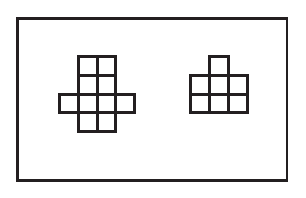
\includegraphics[width=0.73\linewidth]{images/SumPrinc}
\caption{The union of these two disjoint sets has size 17.\label{sumprinc}}
\end{figure}
\begin{figure}
\centering
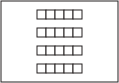
\includegraphics[width=0.73\linewidth]{images/ProdPrinc}
\caption{The union of four disjoint sets of size five.\label{prodprinc}}
\end{figure}
You may have noticed some standard mathematical words and phrases such as \emph{set}, \emph{ordered pair}, \emph{function} and so on creeping into the problems. One of our goals in these notes is to show how most counting problems can be recognized as counting all or some of the elements of a set of standard mathematical objects. For example \hyperref[orderedpair]{Problem~\ref{orderedpair}} is meant to suggest that the question we asked in \hyperref[basicsandwiches]{Problem~\ref{basicsandwiches}} was really a problem of counting all the ordered pairs consisting of a bread choice and a filling choice. We use \(A\times B\) to stand for the set of all ordered pairs whose first element is in \(A\) and whose second element is in \(B\) and we call \(A\times B\) the \index{Cartesian product}\index{product!Cartesian}\terminology{Cartesian product} of \(A\) and \(B\), so you can think of \hyperref[orderedpair]{Problem~\ref{orderedpair}} as asking you for the size of the Cartesian product of \(M\) and \(N\), that is, asking you to count the number of elements of this Cartesian product.%
\par
When a set \(S\) is a union of disjoint sets \(B_1, B_2, \ldots, B_m\) we say that the sets \(B_1, B_2, \ldots, B_m\) are a \terminology{partition}\index{partition!of a set} of the set \(S\). Thus a partition of \(S\) is a (special kind of) set of sets. So that we don't find ourselves getting confused between the set \(S\) and the sets \(B_i\) into which we have divided it, we often call the sets \(B_1, B_2,
\ldots, B_m\) the \emph{blocks}\index{partition!blocks of}\index{block of a partition} of the partition. In this language, the \index{principle!sum}\index{sum principle}\terminology{sum principle}says that%
\begin{quote}if we have a partition of a set \(S\), then the size of \(S\) is the sum of the sizes of the blocks of the partition.\end{quote}
The \index{principle!product}\index{product principle}\terminology{product principle} says that%
\begin{quote}if we have a partition of a set \(S\) into \(m\) blocks, each of size \(n\), then \(S\) has size \(mn\).\end{quote}
You'll notice that in our formal statement of the sum and product pinciple we talked about a partition of a finite set. We could modify our language a bit to cover infinite sizes, but whenever we talk about sizes of sets in what follows, we will be working with finite sets. So as to avoid possible complications in the future, let us agree that when we refer to the size of a set, we are implicitly assuming the set is finite. There is another version of the product principle that applies directly in problems like \hyperref[completelunch]{Problem~\ref{completelunch}} and \hyperref[tripledeckercone]{Problem~\ref{tripledeckercone}}, where we were not just taking a union of \(m\) disjoint sets of size \(n\), but rather \(m\) disjoint sets of size \(n\), each of which was a union of \(m'\) disjoint sets of size \(n'\). This is an inconvenient way to have to think about a counting problem, so we may rephrase the product principle in terms of a sequence of decisions:%
\begin{activity}[]\label{generalproductprincipleintro}
If we make a sequence of \(m\) choices for which \leavevmode%
\begin{itemize}[label=\textbullet]
\item{}there are \(k_1\) possible first choices, and%
\item{}for each way of making the first \(i-1\) choices, there are \(k_i\) ways to make the \(i\)th choice,%
\end{itemize}
 then in how many ways may we make our sequence of choices? (You need not prove your answer correct at this time.)%
\end{activity}
The counting principle you gave in \hyperref[generalproductprincipleintro]{Problem~\ref{generalproductprincipleintro}} is called the \emph{general product principle}.\index{general product principle}\index{product principle!general}\index{principle!product!general} We will outline a proof of the general product pinciple from the original product principle in {$\langle\langle$Unresolved xref, reference "generalproductprincipleproof"; check spelling or use "provisional" attribute$\rangle\rangle$}. Until then, let us simply accept it as another counting principle. For now, notice how much easier it makes it to explain why we multiplied the things we did in \hyperref[completelunch]{Problem~\ref{completelunch}} and \hyperref[tripledeckercone]{Problem~\ref{tripledeckercone}}.%
\begin{activity}[]\label{tennispairings1}
A tennis club has \(2n\) members. We want to pair up the members by twos for singles matches.%
~\par
\begin{enumerate}[label=(\alph*)]
 \item In how many ways may we pair up all the members of the club? (Hint: consider the cases of 2, 4, and 6 members.)%
\par\medskip\noindent%
\textbf{Hint.}\quad Suppose you have a list in alphabetical order of names of the members of the club. In how many ways can you pair up the first person on the list? In how many ways can you pair up the next person who isn’t already paired up?%
\par\medskip\noindent%
\textbf{Solution.}\quad Suppose we list the people in the club in some way, and keep that list for the remainder of the problem. Take the first person from the list and pair that person with any of the \(2n-1\) remaining people. Now take the next \emph{unpaired} person from the list and pair that person with any of the remaining \(2n-3\) unpaired people. Continuing in this way, once \(k\) pairs have been selected, take the next unpaired person from the list and pair that person with any of the remaining \(2n-2k-1\) unpaired people. Every pairing can arise in this way, and no pairing can arise twice in this process. Thus the number of outcomes is \(\prod_{i=0}^{n-1} 2n-2i-1\).%

~\par
\item Suppose that in addition to specifying who plays whom, for each pairing we say who serves first.  Now in how many ways may we specify our pairs?%

\end{enumerate}
\end{activity}
\begin{activity}[]\label{countingfunctions2}
Let us now return to \hyperref[countingfunctions]{Problem~\ref{countingfunctions}} and justify\textemdash{}or perhaps finish\textemdash{}our answer to the question about the number of functions from a three-element set to a 12-element set.%
~\par
\begin{enumerate}[label=(\alph*)]
 \item How can you justify your answer in \hyperref[countingfunctions]{Problem~\ref{countingfunctions}} to the question ``How many functions are there from a three element set (say \([3]=\{1,2,3\}\)) to a twelve element set (say [12])?''%
\par\medskip\noindent%
\textbf{Solution.}\quad The number of functions from \([3]\) to \([12]\) with \(f(3) =1\) is the number of functions from \([2]\) to \([12]\), namely 144. The same is true for the number of functions with \(f(3)=2\) and \(f(3)=3\), and the size of the set \(S_i\). The union of the sets \(S_i\) is the set of all functions from \([3]\) to \([12]\), and since there are twelve sets \(S_i\), this union has size \(12\cdot144= 1728\).%

~\par
\item Based on the examples you've seen so far, make a conjecture about how many functions there are from the set%
\begin{equation*}
[m] = \{1,2,3,\dots,m\}
\end{equation*}
to \([n]=\{1,2,3,\dots,n\}\) and prove it.%
\par\medskip\noindent%
\textbf{Solution.}\quad \(n^m\).%

~\par
\item A common notation for the set of all functions from a set \(M\) to a set \(N\) is \(N^M\).  Why is this a good notation?%
\par\medskip\noindent%
\textbf{Solution.}\quad Because there are \(n^m\) such functions, at least according to our conjecture.%

\end{enumerate}
\end{activity}
\begin{activity}[]\label{generalproductprinciple}
Now suppose we are thinking about a set \(S\) of functions \(f\) from \([m]\) to some set \(X\). (For example, in \hyperref[tripledeckercone]{Problem~\ref{tripledeckercone}} we were thinking of the set of functions from the three possible places for scoops in an ice-cream cone to \(12\) flavors of ice cream.) Suppose there are \(k_1\) choices for \(f(1)\). (In \hyperref[tripledeckercone]{Problem~\ref{tripledeckercone}}, \(k_1\) was \(12\), because there were \(12\) ways to choose the first scoop.) Suppose that for each choice of \(f(1)\) there are \(k_2\) choices for \(f(2)\). (For example, in \hyperref[tripledeckercone]{Problem~\ref{tripledeckercone}} \(k_2\) was \(12\) if the second flavor could be the same as the first, but \(k_2\) was \(11\) if the flavors had to be different.) In general, suppose that for each choice of \(f(1)\), \(f(2)\), \dots{} \(f(i-1)\), there are \(k_i\) choices for \(f(i)\). (For example, in \hyperref[tripledeckercone]{Problem~\ref{tripledeckercone}}, if the flavors have to be different, then for each coice of \(f(1)\) and \(f(2)\), there are \(10\) choices for \(f(3)\).)%
\par
What we have assumed so far about the functions in \(S\) may be summarized as \leavevmode%
\begin{itemize}[label=\textbullet]
\item{}There are \(k_1\) choices for \(f(1)\).%
\item{}For each choice of \(f(1)\), \(f(2)\), \dots{}, \(f(i-1)\), there are \(k_i\) choices for~\(f(i)\).%
\end{itemize}
%
How many functions are in the set \(S\)? Is there any practical difference between the result of this problem and the general product principle?%
\par\medskip\noindent%
\textbf{Solution.}\quad \(\prod_{i=1}^m k_i\).%
\end{activity}
The point of \hyperref[generalproductprinciple]{Problem~\ref{generalproductprinciple}} is that the general product principle can be stated informally, as we did originally, or as a statement about counting sets of standard concrete mathematical objects, namely functions.%
\begin{activity}[]\label{activity-15}
A roller coaster car has \(n\) rows of seats, each of which has room for two people. If \(n\) men and \(n\) women get into the car with a man and a woman in each row, in how many ways may they choose their seats?%
\par\medskip\noindent%
\textbf{Hint.}\quad In how many ways may you assign the men to their rows? The women? Once a woman and a man have a row to share, in how many ways may they choose their seats?%
\par\medskip\noindent%
\textbf{Solution.}\quad \((n!)^22^n\)%
\end{activity}
\begin{activity}[]\label{activity-16}
How does the general product principle apply to \hyperref[tripledeckercone]{Problem~\ref{tripledeckercone}}?%
\par\medskip\noindent%
\textbf{Solution.}\quad By the general product principle, there are \(12\cdot 11\cdot 10\) triple decker cones.%
\end{activity}
\begin{activity}[]\label{activity-17}
In how many ways can we pass out \(k\) distinct pieces of fruit to \(n\) children (with no restriction on how many pieces of fruit a child may get)?%
\par\medskip\noindent%
\textbf{Solution.}\quad Either by the formula for the number of functions from an \(m\)-element set to an \(n\)-element set or the general product principle, there are \(k^n\) ways. (Each distribution is a function from the set of fruit to the set of children, because each piece of fruit goes to one and only one child.)%
\end{activity}
\begin{activity}[]\label{SubsetsFirstTime}
How many subsets does a set \(S\) with \(n\) elements have?%
\par\medskip\noindent%
\textbf{Hint.}\quad Try applying the product principle in the case n = 2 and n = 3. How might you apply it in general?%
\par\medskip\noindent%
\textbf{Solution.}\quad For each of the \(n\) elements of \(S\), we have two options: either we put the element into the subset or we do not. Thus, the general product principle tells us that there are \(2^n\) subsets of \(S\).%
\end{activity}
\begin{activity}[]\label{activity-19}
Assuming \(k\le n\), in how many ways can we pass out \(k\) distinct pieces of fruit to \(n\) children if each child may get at most one? What is the number if \(k>n\)? Assume for both questions that we pass out all the fruit.%
\par\medskip\noindent%
\textbf{Hint.}\quad Ask yourself if either the sum principle or product principle applies.%
\par\medskip\noindent%
\textbf{Hint.}\quad Remember that zero is a number.%
\par\medskip\noindent%
\textbf{Solution.}\quad We are asking for the number of \(k\)-element permutations of \(n\) children, which is \(\prod_{i=1}^k n-i+1\), and is zero if \(k>n\).%
\end{activity}
\begin{activity}[]\label{kelementpermutation}
Another name for a list, in a specific order, of \(k\) distinct things chosen from a set \(S\) is a \terminology{\(k\)-element permutation} of \(S\).\index{permutation!\(k\)-element} We can also think of a \(k\)-element permutation of \(S\) as a one-to-one function (or, in other words, injection) from \([k]=\{1,2,\ldots, k\}\) to \(S\). How many \(k\)-element permutations does an \(n\)-element set have? (For this problem it is natural to assume \(k\le n\). However the question makes sense even if \(k>n\). What is the number of \(k\)-element permutations of an \(n\)-element set if \(k>n\)?%
\par\medskip\noindent%
\textbf{Hint.}\quad Do you see an analogy between this problem and any of the previous problems?%
\par\medskip\noindent%
\textbf{Solution.}\quad By the general product principle, the number is%
\begin{equation*}
\prod_{i=1}^k(n-i+1).
\end{equation*}
In the case that \(k>n\), there are no such lists with distinct entries, and that is what the formula gives us, because \(n-(n+1)+1=0\).%
\end{activity}
There are a number of different notations for the number of \(k\)-element permutations of an \(n\)-element set. The one we shall use was introduced by Don Knuth; namely \(n^{\underline{k}}\), read ``\(n\) to the \(k\) falling'' or ``\(n\) to the \(k\) down''. In \hyperref[kelementpermutation]{Problem~\ref{kelementpermutation}} you may have shown that%
\begin{equation}
n^{\underline{k}} =n(n-1)\cdots (n-k+1)= \prod_{i=1}^k(
n-i+1).\label{productnotation}
\end{equation}
%
\par
It is standard to call \(n^{\underline{k}}\)\index{\(n^{\underline{k}}\)} the \terminology{\(k\)-th falling factorial power of \(n\)}\index{falling factorial power}\index{factorial power!falling}, which explains why we use exponential notation. Of course we call it a \emph{factorial} power since \(n^{\underline{n}} = n(n-1)\cdots 1\) which we call \emph{\(n\)-factorial} and denote by \(n!\).\index{factorial}\index{\(n"!\)} If you are unfamiliar with the \(\Pi\) notation, or \terminology{product notation}\index{product notation}\index{\(Pi\) notation} we introduced for products in \hyperref[productnotation]{Equation~(\ref{productnotation})}, it works just like the \(\Sigma\) notation works for summations.%
\begin{activity}[]\label{activity-21}
Express \(n^{\underline{k}}\) as a quotient of factorials.%
\par\medskip\noindent%
\textbf{Solution.}\quad \(n^{\underline{k}}=n!/(n-k)!\)%
\end{activity}
\begin{activity}[]\label{activity-22}
How should we define \(n^{\underline{0}}\)?%
\par\medskip\noindent%
\textbf{Solution.}\quad We define \(n^{\underline{0}}\) to be \(1\).%
\end{activity}
\typeout{************************************************}
\typeout{Subsection  Functions and directed graphs}
\typeout{************************************************}
\subsection[{Functions and directed graphs}]{Functions and directed graphs}\label{subsection-2}
As another example how standard mathematical language relates to counting problems, \hyperref[countingfunctions]{Problem~\ref{countingfunctions}} explicitly asked you to relate the idea of counting functions to the question of \hyperref[tripledeckercone]{Problem~\ref{tripledeckercone}}. You have probably learned in algebra or calculus how to draw graphs in the Cartesian plane of functions from a set of numbers to a set of numbers. You may recall how we can determine whether a graph is a graph of a function by examining whether each vertical straight line crosses the graph at most one time. You might also recall how we can determine whether such a function is one-to-one by examining whether each horizontal straight line crosses the graph at most one time. The functions we deal with will often involve objects which are not numbers, and will often be functions from one finite set to another. Thus graphs in the cartesian plane will often not be available to us for visualizing functions.%
\par
However, there is another kind of graph called a \emph{directed graph}\index{graph!directed}\index{directed graph} or \emph{digraph}\index{digraph}\index{function!digraph of} that is especially useful when dealing with functions between finite sets. We take up this topic in more detail in {$\langle\langle$Unresolved xref, reference "Relations"; check spelling or use "provisional" attribute$\rangle\rangle$}, particularly {$\langle\langle$Unresolved xref, reference "relationdigraph"; check spelling or use "provisional" attribute$\rangle\rangle$} and {$\langle\langle$Unresolved xref, reference "digraphsoffunctions"; check spelling or use "provisional" attribute$\rangle\rangle$}. In \hyperref[functiondigraphs]{Figure~\ref{functiondigraphs}} we show several examples of digraphs of functions.%
\begin{figure}
\centering
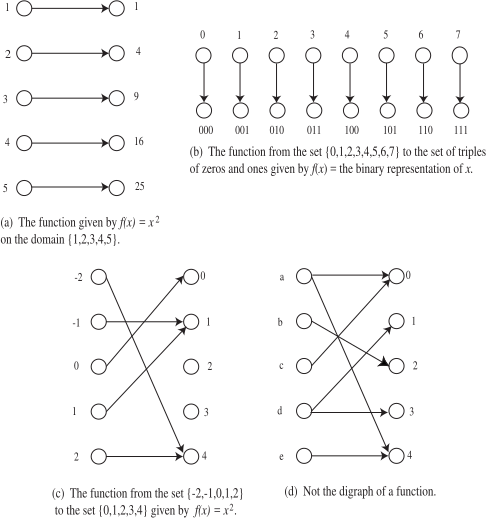
\includegraphics[width=0.73\linewidth]{images/functiondigraph}
\caption{What is a digraph of a function?\label{functiondigraphs}}
\end{figure}
If we have a function \(f\) from a set \(S\) to a set \(T\), we draw a line of dots or circles, called \emph{vertices} to represent the elements of \(S\) and another (usually parallel) line of circles or dots to represent the elements of \(T\). We then draw an arrow from the circle for \(x\) to the circle for \(y\) if \(f(x) = y\). Sometimes, as in part (e) of the figure, if we have a function from a set \(S\) to itself, we draw only one set of vertices representing the elements of \(S\), in which case we can have arrows both entering and leaving a given vertex. As you see, the digraph can be more enlightening in this case if we experiment with the function to find a nice placement of the vertices rather than putting them in a row.%
\par
\emph{The figure needs to have part (e) added to it.}%
\par
Notice that there is a simple test for whether a digraph whose vertices represent the elements of the sets \(S\) and \(T\) is the digraph of a function from \(S\) to \(T\). There must be one and only one arrow leaving each vertex of the digraph representing an element of \(S\). The fact that there is one arrow means that \(f(x)\) is defined for each \(x\) in \(S\). The fact that there is only one arrow means that each \(x\) in \(S\) is related to exactly one element of \(T\). (Note that these remarks hold as well if we have a function from \(S\) to \(S\) and draw only one set of vertices representing the elements of \(S\).) For further discussion of functions and digraphs see {$\langle\langle$Unresolved xref, reference "functionrelation"; check spelling or use "provisional" attribute$\rangle\rangle$} and {$\langle\langle$Unresolved xref, reference "relationdigraph"; check spelling or use "provisional" attribute$\rangle\rangle$} of {{$\langle\langle$Unresolved xref, reference "Relations"; check spelling or use "provisional" attribute$\rangle\rangle$}}.%
\begin{activity}[]\label{activity-23}
Draw the digraph of the function from the set \(\{\)Alice, Bob, Dawn, Bill\(\}\) to the set \(\{\)A, B, C, D, E\(\}\) given by%
\begin{equation*}
f(X) = \mbox{the first
letter of the name \(X\)} .
\end{equation*}
%
\par\medskip\noindent%
\textbf{Solution.}\quad \includegraphics[width=0.73\linewidth]{images/}
%
\end{activity}
\begin{activity}[]\label{activity-24}
A function \(f:S\rightarrow T\) is called an \index{onto function}\index{function!onto}\emph{onto function} or \index{surjection}\index{function!surjection}\emph{surjection} if each element of \(T\) is \(f(x)\) for some \(x\in S\). Choose a set \(S\) and a set \(T\) so that you can draw the digraph of a function from \(S\) to \(T\) that is one-to-one but not onto, and draw the digraph of such a function.%
\par\medskip\noindent%
\textbf{Solution.}\quad The digraph of one such function follows%
\par
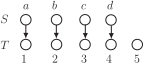
\includegraphics[width=0.73\linewidth]{images/OnetoOneNotOnto}
%
\end{activity}
\begin{activity}[]\label{activity-25}
Choose a set \(S\) and a set \(T\) so that you can draw the digraph of a function from \(S\) to \(T\) that is onto but not one-to-one, and draw the digraph of such a function.%
\par\medskip\noindent%
\textbf{Solution.}\quad The digraph of one such function follows%
\par
\mbox{ \includegraphics[width=0.73\linewidth]{images/OntoNotOnetoOne}
 }%
\end{activity}
\begin{activity}[]\label{activity-26}
Digraphs of functions help us visualize the ideas of one-to-one functions and onto functions.%
~\par
\begin{enumerate}[label=(\alph*)]
 \item What does the digraph of a one-to-one function (injection) from a finite set \(X\) to a finite set \(Y\) look like? (Look for a test somewhat similar to the one we described for when a digraph is the digraph of a function.)%

~\par
\item What does the digraph of an onto function look like?%

~\par
\item What does the digraph of a one-to-one and onto function from a finite set \(S\) to a set \(T\) look like?%

\end{enumerate}
\par\medskip\noindent%
\textbf{Hint.}\quad For each part of this problem, think about how many arrows are allowed to enter a vertex representing a member of \(Y\).\par\medskip\noindent%
\textbf{Solution.}\quad One-to-one: One arrow comes out of each vertex representing a member of \(X\) and at most one arrow goes into each vertex representing a member of \(Y\). Onto: : One arrow comes out of each vertex representing a member of \(X\) and at least one arrow goes into each vertex representing a member of \(Y\). One-to-one and onto: One arrow comes out of each vertex representing a member of \(X\) and at exactly one arrow goes into each vertex representing a member of \(Y\). (The first half of each sentence is optional.)%
\end{activity}
\begin{activity}[]\label{permutationasbijection}
The word \emph{permutation} is actually used in two different ways in mathematics. A \terminology{permutation}\index{permutation!as a bijection} of a set \(S\) is one-to-one from \(S\) onto \(S\). How many permutations does an \(n\)-element set have?%
\par\medskip\noindent%
\textbf{Solution.}\quad \(n!\).%
\end{activity}
Notice that there is a great deal of consistency between the use of the word permutation in \hyperref[permutationasbijection]{Problem~\ref{permutationasbijection}} and the use in \hyperref[kelementpermutation]{Problem~\ref{kelementpermutation}}. If we have some way \(a_1,a_2,\ldots,a_n\) of listing our set, then any other list \(b_1,b_2,\ldots,b_n\) gives us the permutation of \(S\) whose rule is \(f(a_i) =b_i\), and any permutation of \(S\), say the one given by \(g(a_i)=c_i\) gives us a list \(c_1,c_2,\ldots,c_n\) of \(S\). Thus there is really very little difference between the idea of a permutation of \(S\) and an \(n\)-element permutation of \(S\) when \(n\) is the size of \(S\).%
\typeout{************************************************}
\typeout{Subsection  The bijection principle}
\typeout{************************************************}
\subsection[{The bijection principle}]{The bijection principle}\label{subsection-3}
Another name for a one-to-one and onto function is \index{bijection}\index{function!bijection}\terminology{bijection}. The digraphs marked (a), (b), and (e) in \hyperref[functiondigraphs]{Figure~\ref{functiondigraphs}} are digraphs of bijections. The description in \hyperref[bijectiondigraph]{Problem~} of the digraph of a bijection from \(X\) to \(Y\) illustrates one of the fundamental principles of combinatorial mathematics, the \index{principle!bijection}\index{bijection principle}\terminology{bijection principle}:%
\begin{quote}Two sets have the same size if and only if there is a bijection between them.\end{quote}
It is surprising how this innocent sounding principle guides us into finding insight into some otherwise very complicated proofs.%
\typeout{************************************************}
\typeout{Subsection  Counting subsets of a set}
\typeout{************************************************}
\subsection[{Counting subsets of a set}]{Counting subsets of a set}\label{subsection-4}
\begin{activity}[]\label{SubsetsBinaryRepresentation}
The \terminology{binary representation} of a number \(m\) is a list, or string, \(a_1a_2\ldots a_k\) of zeros and ones such that \(m=a_12^{k-1} + a_2 2^{k-2}
+\cdots+ a_k 2^0.\) Describe a bijection between the binary representations of the integers between 0 and \(2^n-1\) and the subsets of an \(n\)-element set. What does this tell you about the number of subsets of an \(n\)-element set?%
\par\medskip\noindent%
\textbf{Hint.}\quad The problem is asking you to describe a one-to-one function from the set of binary representations of numbers between \(0\) and \(2^n-1\) onto the set of subsets of the set \([n]\). Write down these two sets for \(n = 2\). They should both have four elements. The set of binary representations should contain the string \(00\). You could think of this as the instruction ``take no ones and take no twos.'' In that context, what could you think of the string \(11\) as standing for? This should help you describe a function. Of course now you have to figure out how to show it is one-to-one and onto.\par\medskip\noindent%
\textbf{Solution.}\quad The sequence \(a_1a_2\ldots
a_k\) corresponds to the set of \(i\) such that \(a_i = 1\). This is a bijection because each sequence gives a set, and each set can be the set of places where a sequence is 1. Since there are \(2^n\) integers which are between 0 and \(2^n-1\), and they correspond to sequences of length \(n\) (notice, we have another bijection, the one between a number and its binary representation), there are \(2^n\) subsets of the \(n\)-element set \([n]\).%
\end{activity}
Notice that the first question in \hyperref[icecreaminpints]{Problem~\ref{icecreaminpints}} asked you for the number of ways to choose a three element subset from a 12 element subset. You may have seen a notation like \(n\choose k\), \(C(n,k)\), or \(_nC_k\) which stands for the number of ways to choose a \(k\)-element subset from an \(n\)-element set. The number \(n\choose k\) is read as ``\(n\) choose \(k\)'' and is called a \index{binomial coefficient}\terminology{binomial coefficient} for reasons we will see later on. Another frequently used way to read the binomial coefficient notation is ``the number of combinations \index{combinations} of \(n\) things taken \(k\) at a time." You are going to be asked to construct two bijections that relate to these numbers and figure out what famous formula they prove. We are going to think about subsets of the \(n\)-element set \([n] =
\{1,2,3,\ldots, n\}\). As an example, the set of two-element subsets of \([4]\) is%
\begin{equation*}
\{\{1,2\}, \{1,3\}, \{1,4\}, \{2,3\}, \{2,4\}, \{3,4\}\}.
\end{equation*}
%
\par
This example tells us that \({4\choose 2} = 6\).%
\begin{activity}[]\label{Pascal}
Let \(C\) be the set of \(k\)-element subsets of \([n]\) that contain the number \(n\), and let \(D\) be the set of \(k\)-element subsets of \([n]\) that don't contain \(n\).%
~\par
\begin{enumerate}[label=(\alph*)]
 \item Let \(C'\) be the set of \((k-1)\)-element subsets of \([n-1]\).  Describe a bijection from \(C\) to \(C'\).  (A verbal description is fine.)%
\par\medskip\noindent%
\textbf{Solution.}\quad Let \(f(X) = X-\{n\}\), the set \(X\) with \(n\) removed. This is a bijection because two different sets containing \(n\) must yield different sets when \(n\) is removed (one-to-one), and each \((k-1)\)-element subset \(X\) of \([n-1]\) may be obtained from the \(k\)-element subset \(X\cup \{n\}\) of \([n]\) by removing \(n\) (onto).%

~\par
\item Let \(D'\) be the set of \(k\)-element subsets of \([n-1]=\{1,2,\ldots n-1\}\).  Describe a bijection from \(D\) to \(D'\). (A verbal description is fine.)%
\par\medskip\noindent%
\textbf{Solution.}\quad Simply let \(f(X) =X\). This is one-to-one by definition, and onto because the subsets of \([n-1]\) are identical with the subsets of \([n]\) not containing \(n\).%

~\par
\item Based on the two previous parts, express the sizes of \(C\) and \(D\) in terms of binomial coefficients involving \(n-1\) instead of \(n\).%
\par\medskip\noindent%
\textbf{Solution.}\quad \(|C|= {n-1\choose k-1}\); \(|D| = {n-1\choose k}\)%

~\par
\item Apply the sum principle to \(C\) and \(D\) and obtain a formula that expresses \(n\choose k\) in terms of two binomial coefficients involving \(n-1\).  You have just derived the Pascal Equation that is the basis for the famous Pascal's Triangle.%
\par\medskip\noindent%
\textbf{Solution.}\quad \({n\choose k} = {n-1\choose k-1} +{n-1\choose k}\).%

\end{enumerate}
\end{activity}
\typeout{************************************************}
\typeout{Subsection  Pascal's Triangle}
\typeout{************************************************}
\subsection[{Pascal's Triangle}]{Pascal's Triangle}\label{subsection-5}
The Pascal Equation that you derived in \hyperref[Pascal]{Problem~\ref{Pascal}} gives us the triangle in \hyperref[Pascaltriangle]{Figure~\ref{Pascaltriangle}}. This figure has the number of \(k\)-element subsets of an \(n\)-element set as the \(k\)th number over in the \(n\)th row (we call the top row the zeroth row and the beginning entry of a row the zeroth number over). You'll see that your formula doesn't say anything about \(n\choose k\) if \(k=0\) or \(k=n\), but otherwise it says that each entry is the sum of the two that are above it and just to the left or right.%
\begin{figure}
\centering
%
\begin{equation*}
\begin{matrix}\amp \amp \amp \amp \amp \amp \amp 1\amp \amp \amp \amp \amp \amp \amp \\
\amp \amp \amp \amp \amp \amp 1\amp \amp 1\amp \amp \amp \amp \amp \amp \\
\amp \amp \amp \amp \amp 1\amp \amp 2\amp \amp 1\amp \amp \amp \amp \amp \\
\amp \amp \amp \amp 1\amp \amp 3\amp \amp 3\amp \amp 1\amp \amp \amp \amp \\
\amp \amp \amp 1\amp \amp 4\amp \amp 6\amp \amp 4\amp \amp 1\amp \amp \\
\amp \amp 1\amp \amp 5\amp \amp 10\amp \amp 10\amp \amp 5\amp \amp 1\amp \\
\amp 1\amp \amp 6\amp \amp 15\amp \amp 20\amp \amp 15\amp \amp 6\amp \amp 1\\
1\amp \amp 7\amp \amp 21\amp \amp 35\amp \amp 35\amp \amp 21\amp \amp 7\amp \amp 1
\end{matrix}
\end{equation*}
\caption{Pascal's Triangle\label{Pascaltriangle}}
\end{figure}
\index{Pascal's Triangle}%
\begin{activity}[]\label{activity-30}
Just for practice, what is the next row of Pascal's triangle?%
\par\medskip\noindent%
\textbf{Solution.}\quad %
\begin{equation*}
1 \quad 8 \quad 28 \quad 56 \quad 70 \quad 56 \quad 28 \quad 8 \quad 1
\end{equation*}
\end{activity}
\begin{activity}[]\label{activity-31}
Without writing out the rows completely, write out enough of Pascal's triangle to get a numerical answer for the first question in \hyperref[icecreaminpints]{Problem~\ref{icecreaminpints}}.%
\par\medskip\noindent%
\textbf{Hint.}\quad Starting with the row 1 8 28 56 70 56 28 8 1, put dots below it where the elements of row 9 should be. Then put dots below that where the elements of row 10 should be. Do the same for rows 11 and 12. Mark the dot where row 12 should appear. Now mark the dots you need in row 11 to compute the entry in column 3 of row 12. Now mark the dots you need in row 10 to compute the marked entries in row 11. Do the same for rows 9 and 8. Now you should be able to see what you need to do.\par\medskip\noindent%
\textbf{Solution.}\quad Starting with row 9, we get%
\begin{equation*}
\begin{matrix}\amp \amp \amp 1\amp \amp 9\amp \amp 36\amp \amp 84 \cr\amp \amp 1\amp \amp 10\amp \amp 45\amp \amp 120\cr\amp 1\amp \amp 11\amp \amp 55\amp \amp 165\cr
1\amp \amp 12\amp \amp 66\amp \amp 220
\end{matrix}
\end{equation*}
so the answer is 220.%
\end{activity}
It is less common to see Pascal's triangle as a right triangle, but it actually makes your formula easier to interpret. In Pascal's Right Triangle, the element in row \(n\) and column \(k\) (with the convention that the first row is row zero and the first column is column zero) is \(n\choose k\). In this case your formula says each entry in a row is the sum of the one above and the one above and to the left, except for the leftmost and rightmost entries of a row, for which that doesn't make sense. Since the leftmost entry is \(n\choose 0\) and the rightmost entry is \(n\choose n\), these entries are both one (to see why, ask yourself how many \(0\)-element subsets and how many \(n\)-element subsets an \(n\)-element set has), and your formula then tells how to fill in the rest of the table.%
\begin{table}
\centering
\begin{tabular}{lllllllll}
&\(k=0\)&1&2&3&4&5&6&7\tabularnewline[0pt]
&&&&&&&&\tabularnewline\hrulethin
\(n=0\)&1&&&&&&\tabularnewline[0pt]
1&1&1&&&&&\tabularnewline[0pt]
2&1&2&1&&&&&\tabularnewline[0pt]
3&1&3&3&1&&&&\tabularnewline[0pt]
4&1&4&6&4&1&&&\tabularnewline[0pt]
5&1&5&10&10&5&1&&\tabularnewline[0pt]
6&1&6&15&20&15&6&1&\tabularnewline[0pt]
7&1&7&21&35&35&21&7&1
\end{tabular}
\caption{Pascal's Right Triangle\label{Pascalrighttriangle}}
\end{table}
Seeing this right triangle leads us to ask whether there is some natural way to extend the right triangle to a rectangle. If we did have a rectangular table of binomial coefficients, counting the first row as row zero (i.e., \(n=0\)) and the first column as column zero (i.e., \(k=0\)), the entries we don't yet have are values of \(n\choose k\) for \(k>n\). But how many \(k\)-element subsets does an \(n\)-element set have if \(k>n\)? The answer, of course, is zero, so all the other entries we would fill in would be zero, giving us the rectangular array in \hyperref[Pascal_sRectangle]{Figure~\ref{Pascal_sRectangle}}. It is straightforward to check that Pascal's equation now works for all the entries in the rectangle that have an entry above them and an entry above and to the left.%
\begin{table}
\centering
\begin{tabular}{lllllllll}
&\(k=0\)&1&2&3&4&5&6&7\tabularnewline[0pt]
&&&&&&&&\tabularnewline\hrulethin
\(n=0\)&1&0&0&0&0&0&0&0\tabularnewline[0pt]
1&1&1&0&0&0&0&0&0\tabularnewline[0pt]
2&1&2&1&0&0&0&0&0\tabularnewline[0pt]
3&1&3&3&1&0&0&0&0\tabularnewline[0pt]
4&1&4&6&4&1&0&0&0\tabularnewline[0pt]
5&1&5&10&10&5&1&0&0\tabularnewline[0pt]
6&1&6&15&20&15&6&1&0\tabularnewline[0pt]
7&1&7&21&35&35&21&7&1
\end{tabular}
\caption{Pascal's Rectangle\label{Pascal_sRectangle}}
\end{table}
\begin{activity}[]\label{activity-32}
Because our definition told us that \(\binom{n}{k}\) is 0 when \(k>n\), we got a rectangular table of numbers that satisfies the Pascal Equation.%
~\par
\begin{enumerate}[label=(\alph*)]
 \item Is there any other way to define \(n \choose k\) when \(k>n\) in order to get a rectangular table that agrees with Pascal's Right Triangle for \(k\le n\) and satisfies the Pascal Equation?%
\par\medskip\noindent%
\textbf{Hint.}\quad Begin by trying to figure out what the entries just above the diagonal of the rectangle are. After that, what other entries can you figure out?\par\medskip\noindent%
\textbf{Solution.}\quad No, because there must be a zero above each one not in column zero. Then above each zero not in column zero or one, there must be yet another zero and so on.%

~\par
\item Suppose we want to extend Pascal's Rectangle to the left and define \(n\choose -k\) for \(n\ge 0\) and \(k>0\) so that \(-k\lt 0\). What should we put into row \(n\) and column \(-k\) of Pascal's Rectangle in order for the Pascal Equation to hold true?%
\par\medskip\noindent%
\textbf{Hint.}\quad See if you can figure out what the entries in column -1 have to be.\par\medskip\noindent%
\textbf{Solution.}\quad To the left of all the ones in column zero, we must have zeros for the Pascal Equation to hold. To the left of those zeros, we must again have zeros, and so on.%

~\par
\item What should we put into row \(-n\) and column \(k\) or column \(-k\) in order for the Pascal Equation to continue to hold?  Do we have any freedom of choice?%
\par\medskip\noindent%
\textbf{Hint.}\quad What does the sum of two consecutive values in row \(-1\) have to be? Could this sum depend on which two consecutive values we take? Is there some value of row \(-1\) that we could choose arbitrarily? Now what about row \(-2\)? Can we make arbitrary choices there? If so, how many can we make, and is their position arbitrary?\par\medskip\noindent%
\textbf{Solution.}\quad Above row zero, we have some freedom. The \(-1,-1\) and the \(-1,0 \)entry must add to one, so they can be \(-x\) and \(x+1\) for any number \(x\). To the right of the \(-1,0\) entry they must alternate between \((-x-1)\) and \(x+1\) while to the left of the \(-1,1\) entry they must alternate between \(-x\) and \(x\), ending with the \(-x\) in position \(-1,1\). Now if we know the entry in row \(-2\) and column 0, we can use the Pascal equation (in the form \({n-1\choose k-1} = {n\choose k} - {n-1\choose k}\)) to compute all the entries to the left of it, and (in a different form) to compute all the entries to the right of it. Thus we may be arbitrary about the entries in column 0 (or, in fact, one entry in each row) and then the Pascal Equation tells us how to fill in the rest of each row. We shall see later on that there is one very natural choice for how to fill in all the rows above row zero.%

\end{enumerate}
\end{activity}
\begin{activity}[]\label{charfunction}
There is yet another bijection that lets us prove that a set of size \(n\) has \(2^n\) subsets. Namely, for each subset \(S\) of \([n]=\{1,2,\ldots, n\}\), define a function (traditionally denoted by \(\chi_S\)) as follows.\footnote{The symbol \(\chi\) is the Greek letter chi that is pronounced Ki, with the \(i\) sounding like ``eye.''\label{fn-1}}%
\begin{equation*}
\chi_S(i) = \begin{cases}1 \amp \mbox{ if }  i\in S \\ 0 \amp \mbox{ if }  i\not\in
S
\end{cases}
\end{equation*}
%
\par
The function \(\chi_S\) is called the \index{characteristic function}\index{function!characteristic}\terminology{characteristic function} of \(S\). Notice that the characteristic function is a function from \([n]\) to \(\{0,1\}\).%
~\par
\begin{enumerate}[label=(\alph*)]
 \item For practice, consider the function \(\chi_{\{1,3\}}\) for the subset \(\{1,3\}\) of the set \(\{1,2,3,4\}\).  What are \leavevmode%
\begin{enumerate}[label=(\roman*)]
\item\hypertarget{li-5}{}\(\chi_{\{1,3\}}(1)\)?%
\item\hypertarget{li-6}{}\(\chi_{\{1,3\}}(2)\)?%
\item\hypertarget{li-7}{}\(\chi_{\{1,3\}}(3)\)?%
\item\hypertarget{li-8}{}\(\chi_{\{1,3\}}(4)\)?%
\end{enumerate}
%

~\par
\item We define a function \(f\) from the set of subsets of \([n]=\{1,2,\ldots, n\}\) to the set of functions from \([n]\) to \(\{0,1\}\) by \(f(S)=\chi_S\).  Explain why \(f\) is a bijection.%
\par\medskip\noindent%
\textbf{Solution.}\quad If \(i\in S\) but \(i\not\in T\), then \(\chi_S(i)=1\) but \(\chi_T(i)=0\). Thus if \(S\not= T\), the \(\chi_S\not=\chi_T\). Therefore \(f\) is one-to-one. Given a function \(g\) from \([n]\) to \(\{0,1\}\), let \(S=\{i|g(i)=1\}\). Then by definition, \(g=\chi_S=f(S)\). Therefore \(f\) is onto, so it is a bijection.%

~\par
\item Why does the fact that \(f\) is a bijection prove that \([n]\) has \(2^n\) subsets?%
\par\medskip\noindent%
\textbf{Solution.}\quad We have seen that there are \(2^n\) functions from \([n]\) to a two-element set, and we have a bijection between the set of all such functions and the subsets of \([n]\).%

\end{enumerate}
\end{activity}
In \hyperref[SubsetsFirstTime]{Problems~\ref{SubsetsFirstTime}}, \hyperref[SubsetsBinaryRepresentation]{Activity~\ref{SubsetsBinaryRepresentation}}, and \hyperref[charfunction]{Activity~\ref{charfunction}} you gave three proofs of the following theorem.%
\begin{theorem}[{}]\label{theorem-1}
The number of subsets of an \(n\)-element set is \(2^n\).%
\end{theorem}
The proofs in \hyperref[SubsetsBinaryRepresentation]{Problem~\ref{SubsetsBinaryRepresentation}} and \hyperref[charfunction]{Activity~\ref{charfunction}} use essentially the same bijection, but they interpret sequences of zeros and ones differently, and so end up being different proofs. We will give yet another proof, using bijections similar to those we used in proving the Pascal Equation, at the beginning of {$\langle\langle$Unresolved xref, reference "InductionRecursion"; check spelling or use "provisional" attribute$\rangle\rangle$}.%
\typeout{************************************************}
\typeout{Subsection  The quotient principle}
\typeout{************************************************}
\subsection[{The quotient principle}]{The quotient principle}\label{subsection-6}
\begin{activity}[]\label{twelvechoosethree}
As we noted in \hyperref[Pascal]{Problem~\ref{Pascal}}, the first question in \hyperref[icecreaminpints]{Problem~\ref{icecreaminpints}} asked us for the number of three-element subsets of a twelve-element set. We were able to use the Pascal Equation to get a numerical answer to that question. Had we had twenty or thirty flavors of ice cream to choose from, using the Pascal Equation to get our answer would have entailed a good bit more work. We have seen how the general product principle gives us an answer to \hyperref[tripledeckercone]{Problem~\ref{tripledeckercone}}. Thus we might think that the number of ways to choose a three element set from 12 elements is the number of ways to choose the first element times the number of ways to choose the second element times the number of ways to choose the third element, which is \(12\cdot11\cdot10=1320\). However, our result in \hyperref[Pascal]{Problem~\ref{Pascal}} shows that this is wrong.%
~\par
\begin{enumerate}[label=(\alph*)]
 \item What is it that is different between the number of ways to stack ice cream in a triple decker cone with three different flavors of ice cream and the number of ways to simply choose three different flavors of ice cream?%

~\par
\item In particular, how many different triple decker cones use the same three flavors?  (Of course any three distinct flavors could substitute for vanilla, chocolate and strawberry without changing the answer.)%

~\par
\item Using your answer from \hyperref[twelvechoosethreethree]{part~}, compute the number of ways to choose three different flavors of ice cream (out of twelve flavors) from the number of ways to choose a triple decker cone with three different flavors (out of twelve flavors).%

\end{enumerate}
\par\medskip\noindent%
\textbf{Solution.}\quad What is different is that the order in which we put the scoops into the cone matters, but for simply choosing three flavors, the order of the choices doesn't matter. Six different triple decker cones have the same three flavors. Thus we have \(1320/6=220\) different ways to choose three flavors of ice cream from 12 flavors.%
\end{activity}
\begin{activity}[]\label{nchoosek}
Based on what you observed in \hyperref[twelvechoosethreefinal]{Problem~}, how many \(k\)-element subsets does an \(n\)-element set have?%
\par\medskip\noindent%
\textbf{Solution.}\quad Following the reasoning of \hyperref[twelvechoosethree]{Problem~\ref{twelvechoosethree}}, there are \(n^{\underline{k}}\) \(k\)-element permutations of an \(n\)-element set, and \(k!\) of these permutations list the same set of \(k\) elements, so the number of \(k\)-element sets is \({n^{\underline{k}}\over k!}= {n!\over k!(n-k)!}\).%
\end{activity}
\begin{activity}[]\label{activity-36}
The formula you proved in \hyperref[nchoosek]{Problem~\ref{nchoosek}} is symmetric in \(k\) and \(n-k\); that is, it gives the same number for \(n\choose k\) as it gives for \(n\choose n-k\). Whenever two quantities are counted by the same formula it is good for our insight to find a bijection that demonstrates the two sets being counted have the same size. In fact this is a guiding principle of research in combinatorial mathematics. Find a bijection that proves that \(n\choose k\) equals \(n\choose n-k\).%
\par\medskip\noindent%
\textbf{Hint.}\quad The first thing you need to decide is “What are the two sets whose elements we are counting?” Then it will be easier to think of a bijection between these two sets. It turns out that these two sets are sets of sets!\par\medskip\noindent%
\textbf{Solution.}\quad For each \(k\)-element subset \(K\) of the \(n\)-element set \(N\), define \(f(K)\) to be the set of all elements of \(N\) \emph{not} in \(K\). Then \(f\) is the desired bijection.%
\end{activity}
\begin{activity}[]\label{ping-pong}
In how many ways can we pass out \(k\) (identical) ping-pong balls to \(n\) children if each child may get at most one?%
\par\medskip\noindent%
\textbf{Hint.}\quad Ask yourself “What is a problem like this doing in the middle of a bunch of problems about counting subsets of a set? Is it related, or is it supposed to gives us a break from sets?”\par\medskip\noindent%
\textbf{Solution.}\quad \(n\choose k\), because we choose the \(k\) children to whom we give ping-pong balls.%
\end{activity}
\begin{activity}[]\label{roundtable}
In how many ways may \(n\) people sit around a round table? (Assume that when people are sitting around a round table, all that really matters is who is to each person's right. For example, if we can get one arrangement of people around the table from another by having everyone get up and move to the right one place and sit back down, we get an equivalent arrangement of people. Notice that you can get a list from a seating arrangement by marking a place at the table, and then listing the people at the table, starting at that place and moving around to the right.) There are at least two different ways of doing this problem. Try to find them both.%
\par\medskip\noindent%
\textbf{Hint.}\quad The problem suggests that you think about how to get a list from a seating arrangement. Could every list of n distinct people come from a seating chart? How many lists of n distinct people are there? How many lists could we get from a given seating chart by taking different starting places?\par\medskip\noindent%
\textbf{Hint.}\quad Second Hint for Problem 38: For a different way of doing the problem, suppose that you have chosen one person, say the first one in a list of the people in alphabetical order by name. Now seat that person. Does it matter where they sit? In ways can you seat the remaining people? Does it matter where the second person in alphabetical order sits?\par\medskip\noindent%
\textbf{Solution.}\quad The total number of ways to list how the \(n\) people sit around the table is \(n!\). However, two lists are the same if we get one from the other by shifting everyone right the same number of places. This divides the set of lists up into sets of \(n\) mutually equivalent lists. The number \(m\) of such sets is the number of seating arrangements. However by the product principle, \(mn=n!\), because we have partitioned up the set of \(n!\) lists into \(m\) sets of size \(n\). Therefore \(m=(n-1)!\) A second solution may be obtained by choosing one of the \(n\) people and letting this person sit anywhere. Since all that matters is who is to the right of each person, it doesn't matter where this person sits. Once this person is seated, let everybody else sit down. If they sit down first in one order clockwise around the table and then in some other order, the person to the right of somebody has changed. Thus there are \((n-1)!\) ways (the number of ways to seat everybody else) to seat the people around the table.%
\end{activity}
We are now going to analyze the result of \hyperref[nchoosek]{Problem~\ref{nchoosek}} in more detail in order to tease out another counting principle that we can use in a wide variety of situations.%
\begin{table}
\centering
\begin{tabular}{llllll}
\(abc\)&\(acb\)&\(bac\)&\(bca\)&\(cab\)&\(cab\)\tabularnewline[0pt]
\(abd\)&\(adb\)&\(bad\)&\(bda\)&\(dab\)&\(dba\)\tabularnewline[0pt]
\(abe\)&\(aeb\)&\(bae\)&\(bea\)&\(eab\)&\(eba\)\tabularnewline[0pt]
\(acd\)&\(adc\)&\(cad\)&\(cda\)&\(dac\)&\(dca\)\tabularnewline[0pt]
\(ace\)&\(aec\)&\(cae\)&\(cea\)&\(eac\)&\(eca\)\tabularnewline[0pt]
\(ade\)&\(aed\)&\(dae\)&\(dea\)&\(ead\)&\(eda\)\tabularnewline[0pt]
\(bcd\)&\(bdc\)&\(cbd\)&\(cdb\)&\(dbc\)&\(dcb\)\tabularnewline[0pt]
\(bce\)&\(bec\)&\(cbe\)&\(ceb\)&\(ebc\)&\(ecb\)\tabularnewline[0pt]
\(bde\)&\(bed\)&\(dbe\)&\(deb\)&\(ebd\)&\(edb\)\tabularnewline[0pt]
\(cde\)&\(ced\)&\(dce\)&\(dec\)&\(ecd\)&\(edc\)
\end{tabular}
\caption{The \(3\)-element permutations of \(\{a,b,c,d,e\}\) organized by which \(3\)-element set they permute.\label{tab_permsof3}}
\end{table}
In Table~ref{tab:permsof3} we list all three-element permutations of the \(5\)-element set \(\{a,b,c,d,e\}\). Each row consists of all \(3\)-element permutations of some subset of \(\{a,b,c,d,e\}\). Because a given \(k\)-element subset can be listed as a \(k\)-element permutation in \(k!\) ways, there are \(3!=6\) permutations in each row. Because each \(3\)-element permutation appears exactly once in the table, each row is a block of a partition of the set of \(3\)-element permutations of \(\{a,b,c,d,e\}\). Each block has size six. Each block consists of all \(3\)-element permutations of some three-element subset of \(\{a,b,c,d,e\}\). Since there are ten rows, we see that there are ten \(3\)-element subsets of \(\{a,b,c,d,e\}\). An alternate way to see this is to observe that we partitioned the set of all \(60\) three-element permutations of \(\{a,b,c,d,e\}\) into some number \(q\) of blocks, each of size six. Thus by the product principle, \(q\cdot 6=60\), so \(q=10\).%
\begin{activity}[]\label{formulanchoosek}
Rather than restricting ourselves to \(n=5\) and \(k=3\), we can partition the set of all \(k\)-element permutations of \(S\) up into blocks. We do so by letting \(B_K\) be the set (block) of all \(k\)-element permutations of \(K\) for each \(k\)-element subset \(K\) of \(S\). Thus as in our preceding example, each block consists of all permutations of some subset \(K\) of our \(n\)-element set. For example, the permutations of \(\{a,b,c\}\) are listed in the first row of \hyperref[tab_permsof3]{Table~\ref{tab_permsof3}}. In fact each row of that table is a block. The questions that follow are about the corresponding partition of the set of \(k\)-element permutations of \(S\), where \(S\) and \(k\) are arbitrary.%
~\par
\begin{enumerate}[label=(\alph*)]
 \item How many permutations are there in a block?%
\par\medskip\noindent%
\textbf{Hint.}\quad A block consists of all permutations of some subset \(\{a_1 , a_2, \ldots, a_k \}\) of \(S\). How many permutations are there of the set \(\{a_1 , a_2, \ldots, a_k \}\)?
~\par
\item Since \(S\) has \(n\) elements, what does \hyperref[kelementpermutation]{problem~\ref{kelementpermutation}} tell you about the total number of \(k\)-element permutations of \(S\)?%

~\par
\item Describe a bijection between the set of blocks of the partition and the set of \(k\)-element subsets of \(S\).%
\par\medskip\noindent%
\textbf{Hint.}\quad What sets are listed, and how many times is each one listed if you take one list from each row of Table 1.2? How does this choice of lists give you the bijection in this special case?
~\par
\item What formula does this give you for the number \(n\choose k\) of \(k\)-element subsets of an \(n\)-element set?%
\par\medskip\noindent%
\textbf{Hint.}\quad You can make good use of the product principle here.
\end{enumerate}
\par\medskip\noindent%
\textbf{Solution.}\quad The number of permutations in a block is \(k!\). \hyperref[kelementpermutation]{Problem~\ref{kelementpermutation}} tells us that the total number of \(k\)-element permutations is \(n^{\underline{k}}={n!\over (n-k)!}\). Each \(k\)-element set corresponds to the block of all permutations of that set. It is immediate that this is a bijection. Assuming there are \(s\) subsets, we have \(k!s\) permutations in total, so \(k!s={n!\over (n-k)!}\) or \(s= {n!\over k!(n-k)!}\).%
\end{activity}
\begin{activity}[]\label{activity-40}
A basketball team has 12 players. However, only five players play at any given time during a game.%
~\par
\begin{enumerate}[label=(\alph*)]
 \item In how may ways may the coach choose the five players?%

~\par
\item To be more realistic, the five players playing a game normally consist of two guards, two forwards, and one center.  If there are five guards, four forwards, and three centers on the team, in how many ways can the coach choose two guards, two forwards, and one center?%
\par\medskip\noindent%
\textbf{Hint.}\quad The coach is making a sequence of decisions. Can you figure out how many choices the coach has for each decision in the sequence?
~\par
\item What if one of the centers is equally skilled at playing forward?%

\end{enumerate}
\par\medskip\noindent%
\textbf{Hint.}\quad As with any counting problem whose context does not suggest an approach, it is useful to ask yourself if you could decompose the problem into simpler parts by using either the sum or product principle.\par\medskip\noindent%
\textbf{Solution.}\quad \(12\choose 5\). In the more realistic version, \({5\choose2}{4\choose2}{3\choose1}=180\). Finally, either the versatile player is playing center or not, and in the second case is available to play forward. This gives us \({5\choose2}{4\choose2}{1\choose1}+{5\choose2}{5\choose2}{2\choose1}=260\) ways to choose the players.%
\end{activity}
\begin{activity}[]\label{roundtablepartition}
In \hyperref[roundtable]{Problem~\ref{roundtable}}, describe a way to partition the \(n\)-element permutations of the \(n\) people into blocks so that there is a bijection between the set of blocks of the partition and the set of arrangements of the \(n\) people around a round table. What method of solution for \hyperref[roundtable]{Problem~\ref{roundtable}} does this correspond to?%
\par\medskip\noindent%
\textbf{Solution.}\quad Put two permutations in the same block if we can get one from the other by moving everyone (circularly) some number \(r\) places to the right. This corresponds to the method that gives \(n!/n\) as the answer. Many students should be able to answer this question by saying ``See the answer to \hyperref[roundtable]{Problem~\ref{roundtable}}."%
\end{activity}
\begin{activity}[]\label{quotientprinciple}
In \hyperref[formulanchoosekfinal]{Problems~} and \hyperref[roundtablepartition]{Activity~\ref{roundtablepartition}}, you have been using the product principle in a new way. One of the ways in which we previously stated the product principle was ``If we partition a set into \(m\) blocks each of size \(n\), then the set has size \(m\cdot n\).'' In \hyperref[formulanchoosekfinal]{problems~} and \hyperref[roundtablepartition]{Activity~\ref{roundtablepartition}} we knew the size \(p\) of a set \(P\) of permutations of a set, and we knew we had partitioned \(P\) into some unknown number of blocks, each of a certain known size \(r\). If we let \(q\) stand for the number of blocks, what does the product principle tell us about \(p\), \(q\), and \(r\)? What do we get when we solve for \(q\)?%
\par\medskip\noindent%
\textbf{Solution.}\quad \(p=qr\), so that \(q=p/r\).%
\end{activity}
The formula you found in the \hyperref[quotientprinciple]{Problem~\ref{quotientprinciple}} is so useful that we are going to single it out as another principle. The \emph{quotient principle}\index{quotient principle} says:%
\begin{quote}If we partition a set \(P\) into \(q\) blocks, each of size \(r\), then \(q=p/r.\)\end{quote}
The quotient principle is really just a restatement of the product principle, but thinking about it as a principle in its own right often leads us to find solutions to problems. Notice that it does not always give us a formula for the number of blocks of a partition; it only works when all the blocks have the same size. In {$\langle\langle$Unresolved xref, reference "groupsonsets"; check spelling or use "provisional" attribute$\rangle\rangle$}, we develop a way to solve problems with different block sizes in cases where there is a good deal of symmetry in the problem. (The roundness of the table was a symmetry in the problem of people at a table; the fact that we can order the sets in any order is the symmetry in the problem of counting \(k\)-element subsets.)%
\par
In {$\langle\langle$Unresolved xref, reference "equivalencerelations"; check spelling or use "provisional" attribute$\rangle\rangle$} of {$\langle\langle$Unresolved xref, reference "Relations"; check spelling or use "provisional" attribute$\rangle\rangle$} we introduce the idea of an equivalence relation, see what equivalence relations have to do with partitions, and discuss the quotient principle from that point of view. While that appendix is not required for what we are doing here, if you want a more thorough discussion of the quotient principle, this would be a good time to work through that appendix.%
\begin{activity}[]\label{necklace}
In how many ways may we string \(n\) distinct beads on a necklace without a clasp? (Perhaps we make the necklace by stringing the beads on a strong, and then carefully gluing the two ends of the string together so that the joint can't be seen. Assume someone can pick up the necklace, move it around in space and put it back down, giving an apparently different way of stringing the beads that is equivalent to the first.)%
\par\medskip\noindent%
\textbf{Hint.}\quad How could we get a list of beads from a necklace?\par\medskip\noindent%
\textbf{Hint.}\quad When we cut the necklace and string it out on a table, there are 2n lists of beads we could get. Why is it \(2n\) rather than \(n\)?\par\medskip\noindent%
\textbf{Solution.}\quad We can obtain a permutation of the beads by cutting the necklace and stretching it out in a straight line. We can partition the permutations according to which necklace they come from in this process. Two permutations are in the same block if we get one either by circularly permuting the other or by reversing the other (this corresponds to flipping the necklace over in space). Thus each necklace corresponds to \(2n\) permutations so by the quotient principle we have \(n!/2n=(n-1)!/2\) ways to string \(n\) distinct beads on a necklace.%
\end{activity}
\begin{activity}[]\label{tennispairings2}
We first gave this problem as \hyperref[tennispairings1a]{Problem~}. Now we have several ways to approach the problem. A tennis club has \(2n\) members. We want to pair up the members by twos for singles matches.%
~\par
\begin{enumerate}[label=(\alph*)]
 \item In how many ways may we pair up all the members of the club? Give at least two solutions different from the one you gave in \hyperref[tennispairings1a]{Problem~}. (You may not have done \hyperref[tennispairings1a]{Problem~}. In that case, see if you can find three solutions.)%

\par\medskip\noindent%
\textbf{Hint.}\quad You might first choose the pairs of people. You might also choose to make a list of all the people and then take them by twos from the list.~\par
\item Suppose that in addition to specifying who plays whom, for each pairing we say who serves first.  Now in how many ways may we specify our pairs? Try to find as many solutions as you can.%

\end{enumerate}
\par\medskip\noindent%
\textbf{Hint.}\quad You might first choose ordered pairs of people, and have the first person in each pair serve first. You might also choose to make a list of all the people and then take them by twos from the list in order.\par\medskip\noindent%
\textbf{Solution.}\quad Suppose we list the people in the club in some way, and keep that list for the remainder of the problem. Take the first person from the list and pair that person with any of the \(2n-1\) remaining people. Now take the next \emph{unpaired} person from the list and pair that person with any of the remaining \(2n-3\) unpaired people. Continuing in this way, once \(k\) pairs have been selected, take the next unpaired person from the list and pair that person with any of the remaining \(2n-2k-1\) unpaired people. Every pairing can arise in this way, and no pairing can arise twice in this process. Thus the number of outcomes is \(\prod_{i=0}^{n-1} (2n-2i-1)\).%
\par
For another solution, choose people in pairs. There are \(2n\choose 2\) ways to choose one pair, \(2n-2\choose 2\) ways to choose a second pair, and once \(k\) pairs have been chosen, there are \(2n-2k\choose 2\) ways to choose the next pair. The number of \emph{lists} of pairs we get in this way is \(\prod_{i=0}^{n-1}
{2n-2i\choose 2}= {(2n)!\over 2^i}\). However each way of pairing people gets listed \(n!\) times since we see all possible length \(n\) lists of pairs. Therefore the number of actual pairings is \({(2n)!\over 2^n n!}= ={2n!\over
2n\cdot2n-2\cdot2n-4\cdot \cdots\cdot 2} =  \prod_{i=0}^{n-1} 2n-2i-1\).%
\par
For yet another solution, we can list the \(2n\) members in \((2n)!\) ways. Then we can take the first two as a tennis pair, the next two, and so on. There are \(n!\) ways that a given set of tennis pairings could be arranged, and each of the \(n\) pairs could appear in 2 ways, so the tennis pairings partition the set of all permutations of the \(2n\) members into blocks of size \(n!2^n\). Thus we have \((2n)!\over n!2^n\) tennis pairings once again.%
\end{activity}
\begin{activity}[]\label{twocolorsofbeads}
(This becomes especially relevant in {$\langle\langle$Unresolved xref, reference "groupsonsets"; check spelling or use "provisional" attribute$\rangle\rangle$}, though it makes an important point here.) In how many ways may we attach two identical red beads and two identical blue beads to the corners of a square (with one bead per corner) free to move around in (three-dimensional) space?%
\par\medskip\noindent%
\textbf{Hint.}\quad It might be helpful to just draw some pictures of the possible configurations. There aren’t that many.\par\medskip\noindent%
\textbf{Solution.}\quad Two ways; either the red beads are side-by-side or diagonally opposite. If we think about partitioning lists of 2 \(R\)s and 2 \(B\)s so that two are in the same block if we get one from the other by moving the square, we get two blocks, \(\{RRBB, BRRB, BBRR, RBBR\}\) and \(\{RBRB, BRBR\}\).%
\end{activity}
\begin{activity}[]\label{Stirling_sapproximation}
While the formula you proved in \hyperref[nchoosek]{Problems~\ref{nchoosek}} and \hyperref[formulanchoosekfinal]{Task~} is very useful, it doesn't give us a sense of how big the binomial coefficients are. We can get a very rough idea, for example, of the size of \(2n\choose n\) by recognizing that we can write \((2n)^{\underline{n}}/n!\) as \({2n\over n}\cdot
{2n-1\over n-1}\cdots {n+1\over 1}\), and each quotient is at least \(2\), so the product is at least \(2^n\). If this were an accurate estimate, it would mean the fraction of \(n\)-element subsets of a \(2n\)-element set would be about \(2^n/2^{2n}=1/2^n\), which becomes very small as \(n\) becomes large. However it is pretty clear the approximation will not be a very good one, because some of the terms in that product are much larger than 2. In fact, if \(2n\choose k\) were the same for every \(k\), then each would be the fraction \(1\over 2n+1\) of \(2^{2n}\). This is much larger than the fraction \(\frac{1}{2^n}\). But our intuition suggets that \(\binom{2n}{n}\) is much larger than \(\binom{2n}{1}\) and is likely larger than \(\binom{2n}{n-1}\) so we can be sure our approximation is a bad one. For estimates like this, James Stirling developed a formula to approximate \(n!\) when \(n\) is large, namely \(n!\) is about \(\left(\sqrt{2\pi
n}\right){n^n/ e^n}\).\index{Stirling's formula for \(n"!\)}\index{\(n"!\)!Stirling's formula for} In fact the ratio of \(n!\) to this expression approaches 1 as \(n\) becomes infinite.\footnote{Proving this takes more of a detour than is advisable here; however there is an elementary proof which you can work through in the problems of the end of Section 1 of Chapter 1 of \emph{Introductory Combinatorics} by Kenneth P. Bogart, Harcourt Academic Press, (2000).\label{fn-2}} We write this as%
\begin{equation*}
n!\sim \sqrt{2\pi
n}{n^n\over e^n}.
\end{equation*}
%
\par
We read this notation as \(n!\) is asymptotic to \(\sqrt{2\pi n}\frac{n^n}{e^n}\). Use Stirling's formula to show that the fraction of subsets of size \(n\) in an \(2n\)-element set is approximately \(1/\sqrt{\pi n}\). This is a much bigger fraction than \(1\over 2^n\)!%
\end{activity}
\typeout{************************************************}
\typeout{Section 0.3 Some Applications of the Basic Principles}
\typeout{************************************************}
\section[{Some Applications of the Basic Principles}]{Some Applications of the Basic Principles}\label{section-3}
\typeout{************************************************}
\typeout{Subsection  Lattice paths and Catalan Numbers}
\typeout{************************************************}
\subsection[{Lattice paths and Catalan Numbers}]{Lattice paths and Catalan Numbers}\label{subsection-7}
\begin{activity}[]\label{blockwalking}
In a part of a city, all streets run either north-south or east-west, and there are no dead ends. Suppose we are standing on a street corner. In how many ways may we walk to a corner that is four blocks north and six blocks east, using as few blocks as possible?%
\par\medskip\noindent%
\textbf{Hint.}\quad Note that we must walk at least ten blocks, so ten is the smallest number of blocks possible. In how many of those ten blocks must we walk north?%
\par\medskip\noindent%
\textbf{Solution.}\quad The shortest possible walk is going to be ten blocks. To plan a walk, we must choose which four of those ten blocks go north; the other six blocks we will have to go east. There are \(10\choose 4\) ways to make this selection.%
\end{activity}
\begin{activity}[]\label{latticepaths}
\hyperref[blockwalking]{Problem~\ref{blockwalking}} has a geometric interpretation in a coordinate plane. A \emph{lattice path}\index{lattice path}\index{path!lattice} in the plane is a ``curve'' made up of line segments that either go from a point \((i,j)\) to the point \((i+1,j)\) or from a point \((i,j)\) to the point \((i,j+1)\), where \(i\) and \(j\) are integers. (Thus lattice paths always move either up or to the right.) The length of the path is the number of such line segments. What is the length of a lattice path from \((0,0)\) to \((m,n)\)? How many such lattice paths of that length are there? How many lattice paths are there from \((i,j)\) to \((m,n)\), assuming \(i\), \(j\), \(m\), and \(n\) are integers?%
\par\medskip\noindent%
\textbf{Solution.}\quad The length of a lattice path from \((0,0)\) to \((m,n)\) is \(m+n\). The number of such paths is \(m+n\choose n\). Since lattice paths move up and to the right, there are no paths from \((i,j)\) to \((m,n)\) unless \(i\le m\) and \(j\le n\). In that case, the number of paths is \(m+n-i-j\choose n-j\) which is the same as \(m+n-i-j\choose m-i\).%
\end{activity}
\begin{activity}[]\label{diagonallattice}
Another kind of geometric path in the plane is a \emph{diagonal lattice path}\index{lattice path!diagonal}\index{path!lattice!diagonal}. Such a path is a path made up of line segments that go from a point \((i,j)\) to \((i+1,j+1)\) (this is often called an \emph{upstep}) or \((i+1,j-1)\) (this is often called a \emph{downstep}), again where \(i\) and \(j\) are integers. (Thus diagonal lattice paths always move towards the right but may move up or down.) Describe which points are connected to \((0,0)\) by diagonal lattice paths. What is the length of a diagonal lattice path from \((0,0)\) to \((m,n)\)? Assuming that \((m,n)\) is such a point, how many diagonal lattice paths are there from \((0,0)\) to \((m,n)\)?%
\par\medskip\noindent%
\textbf{Solution.}\quad The points \((m,n)\) connected to \((0,0)\) by diagonal lattice paths will have \(m+n\) is even, because each upstep adds two to the sum of \(i\) and \(j\) while each downstep does not change the sum.  Further, since we go one step to the right each time we go up or down, we cannot get above the line \(y=x\) or below the line \(y=-x\). However for any point \((m,n)\) with \(m\) and \(n\) nonnegative integers such that \(m+n\) even and \(-m\le n\le m\), we can get to \(m,n\) by making \(m-n\over 2\) downsteps and \(m+n\over2\) upsteps. In this way we will make a total of \(m\) steps, and our total motion parallel to the \(y\) axis will be \({m+n\over2}-{m-n\over2} = n\).  The length of such a path is \(m\sqrt{2}\); we might informally just call it \(m\) steps. The number of possible paths is the number of ways we can choose which of the \(m\)steps are upsteps (or equivalently downsteps) this number is \(m\choose{m+n\over2}\).%
\end{activity}
\begin{activity}[]\label{activity-50}
A school play requires a ten dollar donation per person; the donation goes into the student activity fund. Assume that each person who comes to the play pays with a ten dollar bill or a twenty dollar bill. The teacher who is collecting the money forgot to get change before the event. If there are always at least as many people who have paid with a ten as a twenty as they arrive the teacher won't have to give anyone an IOU for change. Suppose \(2n\) people come to the play, and exactly half of them pay with ten dollar bills.%
~\par
\begin{enumerate}[label=(\alph*)]
 \item Describe a bijection between the set of sequences of tens and twenties people give the teacher and the set of lattice paths from \((0,0)\) to \((n,n)\).%
\par\medskip\noindent%
\textbf{Solution.}\quad For each ten dollar bill take a rightstep and for each twenty dollar bill take an upstep (where rightstep and upstep have the hopefully natural meaning). The assumption that there are an equal number of ten and twenty dollar bills means that the path will end up at \((n,n)\). Each sequence of tens and twenties gives a lattice path and each lattice path corresponds to such a sequence, so we have a bijection.%

~\par
\item Describe a bijection between the set of sequences of tens and twenties that people give the teacher and the set of diagonal lattice paths from \((0,0)\) and \((0,2n)\).%
\par\medskip\noindent%
\textbf{Solution.}\quad For each ten dollar bill take an upstep and for each twenty dollar bill take a downstep. Each sequence of tens and twenties will give us a diagonal lattice path from \((0,0)\), and each diagonal lattice path from\((0,0)\) to \((0,2n)\) will give us a sequence of tens and twenties with an equal number of tens and twenties, so we have a bijection.%

~\par
\item In each case, what is the geometric interpretation of a sequence that does not require the teacher to give any IOUs?%
\par\medskip\noindent%
\textbf{Solution.}\quad In the first case a sequence that does not require the teacher to give any IOUs will correspond to a lattice path that stays on or below the line \(y=x\), and in the second case such a sequence will correspond to a diagonal lattice path that stays on or above the \(x\)-axis.%

\end{enumerate}
\end{activity}
\begin{activity}[]\label{activity-51}
Notice that a lattice path from \((0,0)\) to \((n,n)\) stays inside (or on the edges of) the square whose sides are the \(x\)-axis, the \(y\)-axis, the line \(x=n\) and the line \(y=n\). In this problem we will compute the number of lattice paths from (0,0) to \((n,n)\) that stay inside (or on the edges of) the triangle whose sides are the \(x\)-axis, the line \(x=n\) and the line \(y=x\). For example, in \hyperref[CatalanPaths]{Figure~\ref{CatalanPaths}} we show the grid of points with integer coordinates for the triangle whose sides are the \(x\)-axis, the line \(x=4\) and the line \(y=x\).%
\begin{figure}
\centering
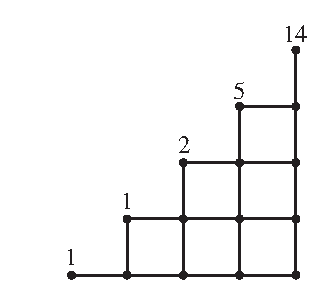
\includegraphics[width=0.33\linewidth]{images/CatalanPaths}
\caption{The lattice paths from \((0,0)\) to \((i,i)\) for \(i=0,1,2,3,4\).  The number of paths to the point \((i,i)\) is shown just above that point.\label{CatalanPaths}}
\end{figure}
~\par
\begin{enumerate}[label=(\alph*)]
 \item Explain why the number of lattice paths from \((0,0)\) to \((n,n)\) that go outside the triangle is the number of lattice paths from \((0,0)\) to \((n,n)\) that either touch or cross the line \(y=x+1\).%
\par\medskip\noindent%
\textbf{Solution.}\quad If a lattice path between \((0,0)\) and \((n,n)\) goes outside the triangle, it can only do so on an upstep. (A step from \((i,j)\) to \((i,j+1)\).) And an upstep must originate at a point with integer coordinates. If \(j\lt i\) an upstep from \((i,j))\) cannot leave the triangle. Thus to leave the triangle, the upstep must leave from a point of the form \((i,i)\), and go to \((i,i+1)\), which is on the line \(y=x+1\).%

~\par
\item Find a bijection between lattice paths from \((0,0)\) to \((n,n)\) that touch (or cross) the line \(y=x+1\) and lattice paths from \((-1,1)\) to \((n,n)\).%
\par\medskip\noindent%
\textbf{Solution.}\quad Suppose we have a lattice path form \((0,0)\) to \((n,n)\) which touches or crosses the line \(y=x+1\). Let \((k,k+1)\) be the first point on the line \(y=x+1\) that the lattice path touches. From that point, work backwards, replacing every upstep with a step one unit to the left and every rightstep with a step one unit down. The segment of the path you just changed will have moved left \(k+1\) times, so its leftmost \(x\) coordinate will be \(-1\), and it will have moved down \(k\) times, so its lowest \(y\) coordinate will be 1.  Thus we now have a lattice path from \((-1,1)\) to \((n,n)\). Further, given a lattice path from \((-1,1)\) to \((n,n)\), it must cross the line \(y=x+1\) at least once, because it starts above the line and ends below it. At the first point where such a path touches the line \(y=x+1\), say \((k',k'+1)\), work backwards replacing every upstep with a step to the left and every rightstep with a step downwards. The leftmost point on this path will have \(x\) coordinate 0, and the lowest point will have \(y\) coordinate 0, so the new path will be a lattice path from \((0,0)\) to \((n,n)\) that touches the line \(y=x+1\). Clearly these two processes reverse each other, and so they give us a bijection between paths form \((0,0)\) to \((n,n)\) that touch the line \(y=x+1\) and lattice lattice paths from \((-1,1)\) to \((n,n)\). Notice that geometrically what we are doing to get the bijection is to take the portion of a lattice path that goes from the initial point till the first touch of the line \(y=x+1\) and reflecting it around that line. This idea of reflection was introduced by Feller, and is called Feller's reflection principle.%

~\par
\item Find a formula for the number of lattice paths from \((0,0)\) to \((n,n)\) that do not cross the line \(y=x\).  The number of such paths is called a \emph{Catalan Number}\index{Catalan Number} and is usually denoted by \(C_n\).%
\par\medskip\noindent%
\textbf{Solution.}\quad \(C_n={2n\choose n} - {2n \choose n+1}={1\over n+1}{2n\choose n}.\)%

\end{enumerate}
\end{activity}
\begin{activity}[]\label{activity-52}
Your formula for the Catalan Number can be expressed as a binomial coefficient divided by an integer. Whenever we have a formula that calls for division by an integer, an ideal combinatorial explanation of the formula is one that uses the quotient principle. The purpose of this problem is to find such an explanation using diagonal lattice paths.\footnote{The result we will derive is called the Chung-Feller Theorem\index{Chung-Feller Theorem}; this approach is based of a paper of Wen-jin Woan ``Uniform Partitions of Lattice Paths and Chung-Feller Generalizations," \textsl{American Mathematics Monthly 58} June/July 2001, p556.\label{fn-3}} A diagonal lattice path that never goes below the \(y\)-coordinate of its first point is called a \terminology{Dyck Path}\index{Dyck path}. We will call a Dyck Path from \((0,0)\) to \((2n,0)\) a \terminology{Catalan Path}\index{Catalan Path} of length \(2n\). Thus the number of Catalan Paths of length \(2n\) is the Catalan Number \(C_n\).%
~\par
\begin{enumerate}[label=(\alph*)]
 \item If a Dyck Path has \(n\) steps (each an upstep or downstep), why do the first \(k\) steps form a Dyck Path for each nonnegative \(k\le n\)?%
\par\medskip\noindent%
\textbf{Solution.}\quad If no points on the path are lower than the first point, then no points among the first \(k\) steps are lower than the first point.%

~\par
\item Thought of as a curve in the plane, a diagonal lattice path can have many local maxima and minima, and can have several absolute maxima and minima, that is, several highest points and several lowest points. What is the \(y\)-coordinate of an absolute minimum point of a Dyck Path starting at \((0,0)\)?  Explain why a Dyck Path whose rightmost absolute minimum point is its last point is a Catalan Path.%
\par\medskip\noindent%
\textbf{Solution.}\quad Since the path starts at \((0,0)\) and can't go below it, the \(y\) coordinate of an absolute minimum must be zero. If the last point is an absolute minimum, then (because it ends with the same \(y\) coordinate with which it starts) the path has an even number \(2k\) of steps and ends at \((2k,0)\).%

~\par
\item Let \(D\) be the set of all diagonal lattice paths from \((0,0)\) to \((2n,0)\).  (Thus these paths can go below the \(x\)-axis.) Suppose we partition \(D\) by letting \(B_i\) be the set of lattice paths in \(D\) that have \(i\) upsteps (perhaps mixed with some downsteps) following the last absolute minimum.  How many blocks does this partition have?  Give a succinct description of the block \(B_0\).%
\par\medskip\noindent%
\textbf{Solution.}\quad The path must have \(n\) upsteps total, and so can have any number between 0 and \(n\) upsteps after the rightmost absolute minimum. Thus the partition has \(n+1\) blocks. Block \(B_0\) consists of the Catalan Paths.%

~\par
\item How many upsteps are in a Catalan Path?%
\par\medskip\noindent%
\textbf{Solution.}\quad \(n\).%

~\par
\item We are going to give a bijection between the set of Catalan Paths and the block \(B_i\) for each \(i\) between \(1\) and \(n\).  For now, suppose the value of \(i\), while unknown, is fixed.  We take a Catalan path and break it into three pieces.  The piece \(F\) (for ``front'') consists of all steps before the \(i\)th upstep in the Catalan path.  The piece \(U\) (for ``up'') consists of the \(i\)th upstep.  The piece \(B\) (for ``back'') is the portion of the path that follows the \(i\)th upstep.  Thus we can think of the path as \(FUB\).  Show that the function that takes \(FUB\) to \(BUF\) is a bijection from the set of Catalan Paths onto the block \(B_i\) of the partition.  (Notice that \(BUF\) can go below the \(x\) axis.)%
\par\medskip\noindent%
\textbf{Solution.}\quad Since we are starting with a Catalan path, the point on the path at the beginning of the \(i\)th upstep must have \(y\) coordinate greater or equal to than zero. Thus wherever we start the sequence \(F\) of upsteps and downsteps, a path constructed by this sequence never goes lower than its starting point. Thus in \(BUF\) the last absolute minimum is either right before the \(U\) or earlier. But \(B\) is the final segment of a Catalan Path, so its final point is at least as low as its starting point. Thus the point at the beginning of the \(U\) in \(BUF\) is an absolute minimum, and there are \(i\) upsteps after that local minimum. If we take two different sequences and rearrange them in the same way, we get two different sequences, so the function we just described is a one-to-one function. If we take an arbitrary diagonal lattice path from \((0,0)\) to \((2n,0)\), let \(U'\) be the first upstep after the last absolute minimum, \(F'\) be the portion of the path that follows \(U'\), and \(B'\) be the portion that precedes \(U'\), then \(F'U'B'\) is a Catalan Path, and \(U'\) is its \(i\)th upstep if and only if in \(B'U'F'\) there are \(i\) upsteps after the last absolute minimum. Thus the mapping from \(FUB\) to \(BUF\) is a bijection.%

~\par
\item Explain how you have just given another proof of the formula for the Catalan Numbers.%
\par\medskip\noindent%
\textbf{Solution.}\quad We have taken the set of all \(2n\choose n\) diagonal lattice paths of length \(2n\) from \((0,0)\) to \((2n,0)\) and partitioned it into \(n+1\) blocks all of size \(C_n\). Thus by the quotient principle, \(C_n={1\over
n+1}{2n
\choose n}\).%

\end{enumerate}
\end{activity}
\typeout{************************************************}
\typeout{Subsection  The Binomial Theorem}
\typeout{************************************************}
\subsection[{The Binomial Theorem}]{The Binomial Theorem}\label{subsection-8}
\begin{activity}[]\label{Conjecturebinomthm}
We know that \((x+y)^2 = x^2+2xy+y^2\). Multiply both sides by \((x+y)\) to get a formula for \((x+y)^3\) and repeat to get a formula for \((x+y)^4\). Do you see a pattern? If so, what is it? If not, repeat the process to get a formula for \((x+y)^5\) and look back at \hyperref[Pascaltriangle]{Figure~\ref{Pascaltriangle}} to see the pattern. Conjecture a formula for \((x+y)^n\).%
\par\medskip\noindent%
\textbf{Solution.}\quad \((x+y)^3=x^3+2x^2y +xy^2+x^2y+ +2xy^2 +y^3=x^3+3x^2y++3xy^2+y^3\).%
\par
Similarly, \((x+4)^4=x^4+4x^3y+6x^2y^2+4xy^3+y^4\),%
\par
and \((x+y)^5=x^5+5x^4y+10x^3y^2+10x^2y^3+5xy^4+y^5.\) The pattern is that the coefficient of \(x^iy^j\) is \(i+j\choose i\) which is the same as \(i+j\choose j\). Said differently, the coefficient of \(x^{n-i}y^i\) is \(n\choose i\) or the coefficient of \(x^iy^{n-i}\) is \(n\choose
i\). We conjecture that%
\begin{equation*}
(x+y)^n=\sum_{i=0}^n {n\choose i}x^{n-i}y^i.
\end{equation*}
%
\par
(The reason for putting \(x^{n-i}y^i\) into the sum is so that as \(i\) goes from 0 to \(n\), the powers of \(x\) decrease from \(n\) to 0.)%
\end{activity}
\begin{activity}[]\label{activity-54}
When we apply the distributive law \(n\) times to \((x+y)^n\), we get a sum of terms of the form \(x^iy^{n-i}\) for various values of the integer \(i\).%
~\par
\begin{enumerate}[label=(\alph*)]
 \item If it is clear to you that each term of the form \(x^iy^{n-i}\) that we get comes from choosing an \(x\) from \(i\) of the \((x+y)\) factors and a \(y\) from the remaining \(n-i\) of the factors and multiplying these choices together, then answer this part of the problem and skip the next part.  Otherwise, do the next part instead of this one.  In how many ways can we choose an \(x\) from \(i\) terms and a \(y\) from \(n-i\) terms?%
\par\medskip\noindent%
\textbf{Solution.}\quad The number of ways to choose an \(x\) from \(i\) of the factors and a \(y\) from the remaining ones is the way to choose the \(i\) factors from the \(n\) factors; that is, \(n\choose i\).%

~\par
\item Expand the product \((x_1 +y_1)(x_2 +y_2)(x_3+y_3)\).%
\par\medskip\noindent%
\textbf{Solution.}\quad %
\begin{align*}
(x_1+y_1)(x_2+y_2)(x_3+y_3)=x_1x_2x_3 \!\!\amp +\amp \!\!x_1x_2y_3+x_1y_2x_3+\\
y_1x_2x_3+x_1y_2y_3+y_1x_2y_3 \!\!\amp +\amp \!\! y_1y_2x_3+y_1y_2y_3.
\end{align*}
%

~\par
\item What do you get when you substitute \(x\) for each \(x_i\) and \(y\) for each \(y_i\)?%
\par\medskip\noindent%
\textbf{Solution.}\quad When you substitute \(x\) for each \(x_i\) and \(y\) for each \(y_i\), you get \((x+y)^3=x^3+3x^2y+3xy^2+y^3\).%

~\par
\item Now imagine expanding%
\begin{equation*}
(x_1+y_1)(x_2+y_2)\cdots (x_n+y_n).
\end{equation*}
Once you apply the commutative law to the individual terms you get, you will have a sum of terms of the form%
\begin{equation*}
x_{k_1}x_{k_2}\cdots x_{k_i}\cdot y_{j_1}y_{j_2}\cdots
y_{j_{n-i}}.
\end{equation*}
What is the set \(\{k_1,k_2,\ldots, k_i\}\cup \{j_1,j_2,\ldots, j_{n-i}\}\)?%
\par\medskip\noindent%
\textbf{Solution.}\quad \(\{k_1,k_2,\ldots, k_i\}\cup
\{j_1,j_2,\ldots, j_{n-i}\}=\{1,2,\ldots, n\}\).%

~\par
\item In how many ways can you choose the set \(\{k_1,k_2,\ldots, k_i\}\)?%
\par\medskip\noindent%
\textbf{Solution.}\quad You can choose the set \(\{k_1,k_2,\ldots k_i\}\) in \(n\choose i\) ways.%

~\par
\item Once you have chosen this set, how many choices do you have for \(\{j_1,j_2,\ldots, j_{n-i}\}\)?%
\par\medskip\noindent%
\textbf{Solution.}\quad Once you have chosen the set of \(k\)s, there is just one way to choose the set of \(j\)s.%

~\par
\item If you substitute \(x\) for each \(x_i\) and \(y\) for each \(y_i\), how many terms of the form \(x^iy^{n-i}\) will you have in the expanded product%
\begin{equation*}
(x_1+y_1)(x_2+y_2)\cdots (x_n+y_n)=(x+y)^n?
\end{equation*}
%
\par\medskip\noindent%
\textbf{Solution.}\quad If you substitute \(x\) for \(x_i\) and substitute \(y\) for \(y_i\), you will get \(n\choose i\) terms of the form \(x^iy^{n-i}\).%

~\par
\item How many terms of the form \(x^{n-i}y^i\) will you have?%
\par\medskip\noindent%
\textbf{Solution.}\quad You will also get \(n\choose i\) terms of the form \(x^{n-i}y^i\).%

~\par
\item Explain how you have just proved your conjecture from \hyperref[Conjecturebinomthm]{Problem~\ref{Conjecturebinomthm}}.  The theorem you have proved is called the \emph{Binomial Theorem}.\index{Binomial Theorem}%
\par\medskip\noindent%
\textbf{Solution.}\quad We have proved that the coefficient of \(x^iy^{n-i}\) in \((x+y)^n\) is \(n\choose i\), or equivalently that the coefficient of \(x^{n-i}y^i\) in \((x+y)^n\) is \(n\choose i\).%

\end{enumerate}
\end{activity}
\begin{activity}[]\label{activity-55}
What is \(\sum_{i=1}^n {10\choose i}3^i\)?%
\par\medskip\noindent%
\textbf{Solution.}\quad \(\sum_{i=1}^n {10\choose i}3^i=\sum_{i=0}^n
{10\choose i}3^i-{10\choose 0}3^0 =(1+3)^{10}-1=4^{10}-1\)%
\end{activity}
\begin{activity}[]\label{activity-56}
What is \({n\choose 0}-{n\choose 1}+{n\choose 2}-\cdots \pm
{n\choose n}\) if \(n\) is an integer bigger than 0?%
\par\medskip\noindent%
\textbf{Solution.}\quad The sum is \(0\) because it is \((-1+1)^n\).%
\end{activity}
\begin{activity}[]\label{activity-57}
Explain why%
\begin{equation*}
\sum_{i=0}^m{m\choose i}{n\choose k-i} = {m+n\choose
k}.
\end{equation*}
Find two different explanations.%
\par\medskip\noindent%
\textbf{Solution.}\quad When we expand both sides of \((x+y)^m(x+y)^n=(x+y)^{m+n}\) by the binomial theorem we get \(\sum_{i=0}^m{m\choose i}{n\choose  k-i}\) as the coefficient of \(x^{m+n-k}y^k\) on the left hand side and \(m+n\choose k\) on the right hand side.%
\par
For a second explanation, to choose \(k\) elements out of the union of an \(m\)-element set and a disjoint \(n\)-element set, chose some number \(i\le m\) of them from the \(m\)-element set and the remaining \(k-i\) of them from the \(n\)-element set. The sum on the left hand side of the equation simply sums the number of such choices over all possible \(i\), and the binomial coefficient on the right hand side of the equation says we will end up choosing \(k\) elements from among our \(m+n\) elements.%
\end{activity}
\begin{activity}[]\label{activity-58}
From the symmetry of the binomial coefficients, it is not too hard to see that when \(n\) is an odd number, the number of subsets of \(\{1,2,\ldots,n\}\) of odd size equals the number of subsets of \(\{1,2,\ldots,n\}\) of even size. Is it true that when \(n\) is even the number of subsets of \(\{1,2,\ldots,n\}\) of even size equals the number of subsets of odd size? Why or why not?%
\par\medskip\noindent%
\textbf{Solution.}\quad It is true, because if \(n>0\), when you expand \((1-1)^n\) by the binomial theorem, you get an alternating sum of binomial coefficients equal to 0, and so the sum of the binomial coefficients \(n\choose i\) with \(i\) even must equal the sum of the binomial coefficients \(n\choose i\) with \(i\) odd.%
\end{activity}
\begin{activity}[]\label{activity-59}
What is \(\sum_{i=0}^n i{n\choose i}\)? (Hint: think about how you might use calculus.)%
\par\medskip\noindent%
\textbf{Solution.}\quad \(\sum_{i=0}^n({n\choose i}x^i = (1+x)^n\). Taking derivatives of both sides gives us \(\sum_{i=0}^ni{n\choose i}x^{i-1} = n(1+x)^{n-1}.\). Now substitute 1 for \(x\) and you get \(\sum_{i=0}^n i{n\choose i} = n2^{n-1}\).%
\end{activity}
Notice how the proof you gave of the binomial theorem was a counting argument. It is interesting that an apparently algebraic theorem that tells us how to expand a power of a binomial is proved by an argument that amounts to counting the individual terms of the expansion. Part of the reason that combinatorial mathematics turns out to be so useful is that counting arguments often underlie important results of algebra. As the algebra becomes more sophisticated, so do the families of objects we have to count, but nonetheless we can develop a great deal of algebra on the basis of counting.%
\typeout{************************************************}
\typeout{Subsection  The pigeonhole principle}
\typeout{************************************************}
\subsection[{The pigeonhole principle}]{The pigeonhole principle}\label{subsection-9}
\begin{activity}[]\label{elevencoins}
American coins are all marked with the year in which they were made. How many coins do you need to have in your hand to guarantee that on two (at least) of them, the date has the same last digit? (When we say ``to guarantee that on two (at least) of them,\dots{}'' we mean that you can find two with the same last digit. You might be able to find three with that last digit, or you might be able to find one pair with the last digit 1 and one pair with the last digit 9, or any combination of equal last digits, as long as there is at least one pair with the same last digit.)%
\par\medskip\noindent%
\textbf{Solution.}\quad Since there are ten possible last digits, you need at least 11 coins, and with 11 coins, at least two last digits must be the same.%
\end{activity}
There are many ways in which you might explain your answer to \hyperref[elevencoins]{Activity~\ref{elevencoins}}. For example, you can partition the coins according to the last digit of their date; that is, you put all the coins with a given last digit in a block together, and put no other coins in that block; repeating until all coins are in some block. Then you have a partition of your set of coins. If no two coins have the same last digit, then each block has exactly one coin. Since there are only ten digits, there are at most ten blocks and so by the sum principle there are at most ten coins. In fact with ten coins it is possible to have no two with the same last digit, but with 11 coins some block must have at least two coins in order for the sum of the sizes of at most ten blocks to be 11. This is one explanation of why we need 11 coins in \hyperref[elevencoins]{Activity~\ref{elevencoins}}. This kind of situation arises often in combinatorial situations, and so rather than always using the sum principle to explain our reasoning , we enunciate another principle which we can think of as yet another variant of the sum principle. The \terminology{pigeonhole principle}\index{pigeonhole principle} states that%
\begin{quote}If we partition a set with more than \(n\) elements into \(n\) parts, then at least one part has more than one element.%
\end{quote}
The pigeonhole principle gets its name from the idea of a grid of little boxes that might be used, for example, to sort mail, or as mailboxes for a group of people in an office. The boxes in such grids are sometimes called pigeonholes in analogy with stacks of boxes used to house homing pigeons when homing pigeons were used to carry messages. People will sometimes state the principle in a more colorful way as ``if we put more than \(n\) pigeons into \(n\) pigeonholes, then some pigeonhole has more than one pigeon.''%
\begin{activity}[]\label{activity-61}
Show that if we have a function from a set of size \(n\) to a set of size less than \(n\), then \(f\) is not one-to-one.%
\par\medskip\noindent%
\textbf{Solution.}\quad Let \(T\) be the set of size less than \(n\), and \(S\) be the set of size \(n\). Let \(B_j=\{i|f(i)=j\}\) for each \(j\) in \(T\). Then the nonempty sets among the \(B_j\)s form a partition of \(S\) and the number of blocks is less than the size of \(S\). Therefore by the pigeonhole principle, there is at least one block with at least two elements, so there are two elements \(i_1\) and \(i_2\) such that \(f(i_1)=f(i_2)\).%
\end{activity}
\begin{activity}[]\label{activity-62}
Show that if \(S\) and \(T\) are finite sets of the same size, then a function \(f\) from \(S\) to \(T\) is one-to-one if and only if it is onto.%
\par\medskip\noindent%
\textbf{Solution.}\quad First suppose that \(f\) is a one-to-one function from \(S\) to \(T\), sets which have the same size. Let \(B_j=\{i|f(i)=j\}\) for each \(j\) in \(T\)..  If \(f\) is not onto, then the number of nonempty sets \(B_j\) is smaller than the number of elements of \(T\) and thus is smaller than the size of \(S\). The nonempty sets \(B_j\) are a partition of \(S\). But then by the pigeonhole principle, some nonempty \(B_j\) has two or more elements, contradicting the assumption that \(f\) is one-to-one. Therefore if \(f\) is one-to-one, then it is onto. Now suppose that \(f\) is an onto function from \(S\) to \(T\), sets of the same size. Again let \(B_j =\{i|f(i)=j\}\) for each \(j\) in \(T\). The size of the union of the sets \(B_j\) is, by the sum principle, the sum of their sizes. Since \(f\) is onto, each \(B_j\) has at least one element. Since the number of sets \(B_j\) is the number of elements of \(S\), if one of those sets has more than one element, the the size of their union is more than the size of \(S\), which is a contradiction since they are subsets of \(S\). Therefore each set \(B_j\) has exactly one element and therefore \(f\) is one-to-one.%
\end{activity}
\begin{activity}[]\label{activity-63}
~\par
\begin{enumerate}[label=(\alph*)]
 \item There is a \terminology{generalized pigeonhole principle}\index{pigeonhole principle!generalized} which says that if we partition a set with more than \(kn\) elements into \(n\) blocks, then at least one block has at least \(k+1\) elements. Prove the generalized pigeonhole principle.%
\par\medskip\noindent%
\textbf{Solution.}\quad Suppose we partition a set \(S\) of more than \(kn\) elements into \(n\) blocks. If each block has at most \(k\) elements, the by the sum principle the size of \(S\) is at most \(kn\). But this is a contradiction, so some block has at least \(k+1\) elements.%

~\par
\item All the powers of five end in a five, and all the powers of two are even. Show that for for some integer \(n\), if you take the first \(n\) powers of a prime other than two or five, one must have ``01'' as the last two digits.%
\par\medskip\noindent%
\textbf{Solution.}\quad If we take 40 powers of such a prime, either one will end in ``01'' or some two, say \(p^i\) and \(p^j\) with \(i>j\) must have the same last two digits by the pigeon hole principle. Then \(p^i-p^j=100k\) for some integer \(k\). Thus \(p^j(p^{i-j} -1)\) must be a multiple of 100, and since neither 2 nor 5 divide \(p\), \(p^{i-j} -1 = 100k'\) for some integer \(k'\) then \(p^{i-j} = 100k'+1\), so the last two digits of \(p^{i-j}\) must be ``01.''%

\end{enumerate}
\end{activity}
\begin{activity}[]\label{R_3_3_}
Show that in a set of six people, there is a set of at least three people who all know each other, or a set of at least three people none of whom know each other. (We assume that if person 1 knows person 2, then person 2 knows person 1.)%
\par\medskip\noindent%
\textbf{Solution.}\quad By the generalized pigeonhole principle, person 1 either knows at least three people or doesn't know at least three people. Suppose person 1 knows three people. Then either two of these people know each other, giving us, with person 1, three mutual acquaintances, or no two of these people know each other, giving us three mutual strangers. On the other hand if there are three people person 1 does not know, then either two of these people don't know each other, giving us, with person 1, three mutual strangers, or all three of these people know each other, giving us three mutual acquaintances.%
\end{activity}
\begin{activity}[]\label{notR_3_3_}
Draw five circles labeled Al, Sue, Don, Pam, and Jo. Find a way to draw red and green lines between people so that every pair of people is joined by a line and there is neither a triangle consisting entirely of red lines or a triangle consisting of green lines. What does \hyperref[R_3_3_]{Problem~\ref{R_3_3_}} tell you about the possibility of doing this with six people's names? What does this problem say about the conclusion of \hyperref[R_3_3_]{Problem~\ref{R_3_3_}} holding when there are five people in our set rather than six?%
\par\medskip\noindent%
\textbf{Solution.}\quad In the figure that follows, we use solid lines for red and dashed lines for green. Clearly there is no solid triangle and no dashed triangle.%
\begin{figure}
\centering
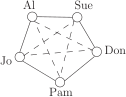
\includegraphics[width=0.33\linewidth]{images/NonRamsey5}
\end{figure}
\hyperref[R_3_3_]{Activity~\ref{R_3_3_}} says you can't do this with six people's names. This problem says that the conclusion of \hyperref[R_3_3_]{Activity~\ref{R_3_3_}} does not hold when you have five people.%
\end{activity}
\typeout{************************************************}
\typeout{Subsection  Ramsey Numbers}
\typeout{************************************************}
\subsection[{Ramsey Numbers}]{Ramsey Numbers}\label{Ramseysection}
Activity~\hyperref[R_3_3_]{\ref{R_3_3_}}--\hyperref[notR_3_3_]{\ref{notR_3_3_}} together show that six is the smallest number \(R\) with the property that if we have \(R\) people in a room, then there is either a set of (at least) three mutual acquaintances or a set of (at least) three mutual strangers. Another way to say the same thing is to say that six is the smallest number so that no matter how we connect 6 points in the plane (no three on a line) with red and green lines, we can find either a red triangle or a green triangle. There is a name for this property. The \terminology{Ramsey Number} \(R(m,n)\) is the smallest number \(R\) so that if we have \(R\) people in a room, then there is a set of at least \(m\) mutual acquaintances or at least \(n\) mutual strangers. There is also a geometric description of Ramsey Numbers; it uses the idea of a \emph{complete graph} on \(R\) vertices. A \emph{complete graph}\index{graph!complete} on \(R\) vertices consists of \(R\) points in the plane together with line segments (or curves) connecting each two of the \(R\) vertices.\footnote{As you may have guessed, a complete graph is a special case of something called a graph.  The word graph will be defined in {$\langle\langle$Unresolved xref, reference "graphsection"; check spelling or use "provisional" attribute$\rangle\rangle$}.\label{fn-4}} The points are called \terminology{vertices}\index{vertex!of a complete graph}\index{vertex} and the line segments are called \terminology{edges}\index{edge!of a complete graph}\index{edge}. In \hyperref[completegraph]{Figure~\ref{completegraph}} we show three different ways to draw a complete graph on four vertices. We use \(K_n\) to stand for a complete graph on \(n\) vertices.%
\begin{figure}
\centering
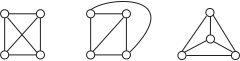
\includegraphics[width=0.33\linewidth]{images/threeK4s}
\caption{Three ways to draw a complete graph on four vertices\label{completegraph}}
\end{figure}
Our geometric description of \(R(3,3)\) may be translated into the language of graph theory (which is the subject that includes complete graphs) by saying \(R(3,3)\) is the smallest number \(R\) so that if we color the edges of a \(K_R\) with two colors, then we can find in our picture a \(K_3\) all of whose edges have the same color.  The graph theory description of \(R(m,n)\) is that \(R(m,n)\) is the smallest number \(R\) so that if we color the edges of a \(K_R\) with red and green, then we can find in our picture either a \(K_m\) all of whose edges are red or a \(K_n\) all of whose edges are green. Because we could have said our colors in the opposite order, we may conclude that \(R(m,n) = R(n,m)\). In particular \(R(n,n)\) is the smallest number \(R\) such that if we color the edges of a \(K_R\) with two colors, then our picture contains a \(K_n\) all of whose edges have the same color.%
\begin{activity}[]\label{activity-66}
Since \(R(3,3)=6\), an uneducated guess might be that \(R(4,4)=8\). Show that this is not the case.%
\par\medskip\noindent%
\textbf{Solution.}\quad In the graph of \hyperref[NonRamsey8]{Figure~\ref{NonRamsey8}}, each vertex has three dashed lines emanating from it, and there are no dashed lines connecting any of the three vertices adjacent to it by dashed lines. Each vertex has four solid lines emanating from it, and no three of the four vertices adjacent to it by solid lines are all adjacent by solid lines. Thus there is no solid line \(K_4\) and there is no dashed line \(K_4\).%
\begin{figure}
\centering
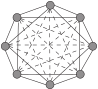
\includegraphics[width=0.33\linewidth]{images/NonRamsey8}
\caption{A graph showing \(R(4,4) \gt 8\)\label{NonRamsey8}}
\end{figure}
\end{activity}
\begin{activity}[]\label{activity-67}
Show that among ten people, there are either four mutual acquaintances or three mutual strangers. What does this say about \(R(4,3)\)?%
\par\medskip\noindent%
\textbf{Solution.}\quad Take a person, say person 1. If person has six acquaintances, then by \hyperref[R_3_3_]{Activity~\ref{R_3_3_}} among them there are either three mutual strangers, in which case we are done, or three mutual acquaintances. These three acquaintances together with person 1 form a set of 4 mutual acquaintances in which case we are again done. Thus we may assume Person 1 has at most 5 acquaintances, and so has four non-acquaintances. Now either all four of these people are acquainted, in which case we are done, or else two of them are not acquainted. Then these two people, together with person 1 make three mutual nonacquaintances. Therefore in every possible case, we have either four mutual acquaintances or three mutual strangers. This means that \(R(4,3) \le 10\).%
\end{activity}
\begin{activity}[]\label{OddNoPeople}
Show that among an odd number of people there is at least one person who is an acquaintance of an even number of people and therefore also a stranger to an even number of people.%
\par\medskip\noindent%
\textbf{Solution.}\quad Suppose we add, for each person, the number of people with whom he or she is acquainted. Then we get twice the number of acquaintance edges in the graph of acquaintance and non-acquaintance relationships. Thus the sum must be even. But if each person among an odd number of people were acquainted with an odd number of people, then the sum would be odd. Since this is a contradiction, among an odd number of people, there must be at least one who is acquainted with an even number of people. Since the number of people different from this person is even, the number of people with whom this person is not acquainted is also even.%
\end{activity}
\begin{activity}[]\label{R_4_3_not8}
Find a way to color the edges of a \(K_8\) with red and green so that there is no red \(K_4\) and no green \(K_3\).%
\par\medskip\noindent%
\textbf{Solution.}\quad In the graph shown in \hyperref[NonRamsey8]{Figure~\ref{NonRamsey8}}, there is no \(K_3\) whose edges are dashed, and no \(K_4\) whose edges are solid. By symmetry, to verify this you need only look at vertex 1 and vertices connected to it by either dashed lines or by solid lines.%
\end{activity}
\begin{activity}[]\label{activity-70}
Find \(R(4,3)\).%
\par\medskip\noindent%
\textbf{Solution.}\quad \(R(4,3)=9\). In \hyperref[R_4_3_not8]{Activity~\ref{R_4_3_not8}} we showed that \(R(4,3)\) is more than 8. So we must show that if we have nine people, we either have 4 mutual acquaintances or three mutual strangers. By \hyperref[OddNoPeople]{Activity~\ref{OddNoPeople}} there is at least one person (say person A) who is acquainted with an even number of people. If person A is acquainted with six or more people, then among these six people, there are either three mutual acquaintances or three mutual strangers. If there are three mutual strangers, we are done; if there are three mutual acquaintances, they, together with Person A are four mutual acquaintances. Thus we may assume Person A is acquainted with at most four people. Thus person A is a stranger to at least four people. If two of these people are strangers, then they, together with person A form three mutual strangers and we are done. Otherwise all of these people know each other and we have at least four mutual acquaintances, and so in every possible situation, we have either four mutual acquaintances or three mutual strangers.%
\end{activity}
As of this writing, relatively few Ramsey Numbers are known. \(R(3,n)\) is known for \(n\lt 10\), \(R(4,4) = 18\), and \(R(5,4)=R(4,5)=25\).%
\typeout{************************************************}
\typeout{Section 0.4 Supplementary Chapter Problems}
\typeout{************************************************}
\section[{Supplementary Chapter Problems}]{Supplementary Chapter Problems}\label{section-4}
\leavevmode%
\begin{enumerate}
\item\hypertarget{compositiondefinition}{}(interesting) Remember that we can write \(n\) as a sum of \(n\) ones.  How many plus signs do we use?  In how many ways may we write \(n\) as a sum of a list of \(k\) positive numbers?  Such a list is called a \emph{composition}\index{composition} of \(n\) into \(k\) parts.\index{composition!\(k\) parts}\index{composition!\(k\) parts!number of} We use \(n-1\) plus signs. Write down such a sum and choose \(k-1\) of the plus signs. Then each string of ones and plusses between two chosen plus signs, before the first chosen plus sign or after the last chosen one corresponds to a part of a composition of \(n\). Thus the number of compositions of \(n\) with \(k\) parts is the number of ways to choose the \(k-1\) places, which is \(n-1\choose k-1\).%
%
\item\hypertarget{composition_numberof}{}In \hyperlink{compositiondefinition}{Problem~1} we defined a composition of \(n\) into \(k\) parts.  What is the total number of compositions of \(n\) (into any number of parts). \index{compositions!number of} The total number of compositions is the number of ways to choose a subset of the plus signs which is \(2^{n-1}\).%
%
\item\hypertarget{GreyCode}{}(essential for this or the next section) Write down a list of all 16 0-1 sequences of length four starting with 0000 in such a way that each entry differs from the precious one by changing just one digit.  This is called a Grey Code.\index{Grey Code}  That is, a \emph{Grey Code} for 0-1 sequences of length \(n\) is a list of the sequences so that each entry differs from the previous one in exactly one place.  Can you describe how to get a Grey Code for 0-1 sequences of length five from the one you found for sequences of length 4?  Can you describe how to prove that there is a Grey code for sequences of length \(n\)? (One of many) 0000, 0001, 0011, 0010, 0110, 0111, 0101, 0100, 1100, 1101, 1111, 1110, 1010, 1011, 1001, 1000. To get a code for sequences of length 5, put a zero at the end of each of the sequences we have. Follow that revised sequence by 10001, and write the remainder of the sequence in reverse order with a 1 at the end of each term. (Don't reverse the individual length four sequences, just the sequence of sequences!) We just, in essence, described the inductive step of an inductive proof that Grey Codes exist for sequences of any length.%
%
\item\hypertarget{li-12}{}(interesting) Use the idea of a Grey Code from \hyperlink{GreyCode}{Problem~3} to prove bijectively that the number of even-sized subsets of an \(n\)-element set equals the number of odd-sized subsets of an \(n\)-element set. Each sequence in the Grey Code is the characteristic function of a set, and the number of elements of the set is the number of ones in the sequence. Since each sequence differs in just one place from the preceding one, the sequences alternate between having an even number of ones and an odd number of ones. Since the first sequence is all zeros and there are \(2^n\) sequences, the last one has an odd number of zeros. Thus the map that takes each sequence except the last to the next one, and takes the last to the first is a bijection between the characteristic functions of sets with an even number of elements and sets with an odd number of elements.%
%
\item\hypertarget{li-13}{}(interesting) A list of parentheses is said to be balanced if there are the same number of left parentheses as right, and as we count from left to right we always find at least as many left parentheses as right parentheses.  For example, (((()()))()) is balanced and ((()) and (()()))(() are not.  How many balanced lists of \(n\) left and \(n\)  right parentheses are there? The number is the Catalan number: we get a bijection between balanced lists of parentheses and Catalan paths by sending each left paren to an upstep and each right paren to a downstep. The condition that there are always as many left parentheses as right ensures we never go below the \(x\) axis.%
%
\item\hypertarget{li-14}{}(difficult) Suppose we plan to put six distinct computers in a network as shown in \hyperref[hexagonalnetwork]{Figure~\ref{hexagonalnetwork}}.  The lines show which computers can communicate directly with which others.  Consider two ways of assigning computers to the nodes of the network different if there are two computers that communicate directly in one assignment and that don't communicate directly in the other.  In how many different ways can we assign computers to the network? \begin{figure}
\centering
\includegraphics[width=0.73\linewidth]{images/}
\caption{A computer network.\label{hexagonalnetwork}}
\end{figure}
 We consider two assignments of computers to be equivalent if in both assignments, each computer communicates directly with exactly the same computers. This partitions the set of all \(6!\) computer assignments into blocks of \(48\) computers each. Thus we have \(720/48=15\) ways to assign the computers to the network.%
%
\item\hypertarget{li-15}{}(interesting) In a circular ice cream dish we are going to put four distinct scoops of ice cream chosen from among twelve flavors.  Assuming we place four scoops of the same size as if they were at the corners of a square, and recognizing that moving the dish doesn't change the way in which we have put the ice cream into the dish, in how many ways may we choose the ice cream and put it into the dish? Each ice cream arrangement is equivalent to three others, the ones we get by rotating the dish. This divides the arrangements of four flavors of ice cream into blocks of size 4. Thus we may arrange the ice cream we have chosen in the dish in \(4!/4=6\) ways. We may choose the ice cream in \({12\choose 4}=495\) ways, and so we may choose it and put it into the dish in 2970 ways.%
%
\item\hypertarget{li-16}{}(interesting) In as many ways as you can, show that \({n\choose k}{n-k\choose m} =
{n\choose m}{n-m\choose k}\). You can prove this by plugging in the formula for \(n\choose k\) on both sides and cancelling stuff until you get the same thing on both sides. However a much more interesting proof is that the right hand side counts the number of ways to choose a \(k\)-element set form an \(n\)-element set and then choose an \(m\)-element set from what remains. The left hand side counts the number of ways to first chose a \(k\)-element subset from the \(n\)-element set and then choose an \(m\)-element subset from what remains. Thus in both cases you are counting the number of ways to choose an ordered pair consisting of an \(m\)-element subset and a disjoint \(k\)-element subset from an \(n\)-element set. You can also base a proof on the observation that \((x+y+x)^n=
\sum_{k=0}^n{n\choose k}(x+y)^kz^{n-k}\) and \((x+y+z)^n=\sum_{m=0}^n{n\choose m}x^m(y+z)^{n-m}\) and asking for the coefficient of \(x^my^{n-m-k}z^k\). You do have to use the binomial theorem with an eye to the result you are looking for, however.%
%
\item\hypertarget{li-17}{}(interesting) A tennis club has \(4n\) members.  To specify a doubles match, we choose two teams of two people.  In how many ways may we arrange the members into doubles matches so that each player is in one doubles match?  In how many ways may we do it if we specify in addition who serves first on each team? We now have many methods for solving this problem. Perhaps the easiest is to list all \((4n)\) people and take them in groups of four for doubles matches, with the first two in a group of four as one team and the second two as another team. We note that interchanging the \(n\) blocks of 4 does not change the matches, nor does interchanging the two people on a team nor interchanging the two teams. Thus we have \((4n)!/n!2^{3n}\) ways to arrange the matches. If we are to say who serves first on each team, we might as well say it is the first of the two listed, so now we have \((4n)!/n!2^n\) ways to arrange the matches.%
%
\item\hypertarget{li-18}{}A town has \(n\) streetlights running along the north side of main street.  The poles on which they are mounted need to be painted so that they do not rust.  In how many ways may they be painted with red, white, blue, and green if an even number of them are to be painted green? We can think of first choosing the set of even size of poles to be painted green, and the painting the remaining poles red, white, and blue. We may do this in \(\sum_{k=0}^{\lfloor n/2\rfloor}{n\choose 2k}3^{n-2k}\) ways.%
%
\item\hypertarget{pingpongpaint}{}We have \(n\) identical ping-pong balls.  In how many ways may we paint them red, white, blue, and green? We can line up the identical ping-pong balls and break them into four groups, those of each color, by inserting dividers. If we want to paint at least one in each color, we can choose three of the spaces between the balls in which to insert dividers, so we can paint them in \(n-1\choose k\). But the problem didn't require us to use each color, so we can put two dividers adjacent to each other. Thus there are \(n+1\) places where we can put the first divider (putting it before all the balls means we use no red, and putting it after all of them means we use no green. Now there are \(n+2\) places where we can put the second divider, including before or after the first, and \(n+3\) places where we can put the third divider. However if we interchange two dividers we still paint the balls before the first divider red, those between then next two white, and so on. Thus \(3!=6\) of these arrangements of balls and dividers correspond to the same paint job, so the number of ways to paint the balls is \({(n+1)(n+2)(n+3)\over6} ={n+3\choose
3}\). This suggests that another way to think of the problem is to consider \(n+3\) slots in a row, and fill \(n\) of them with balls and \(3\) of them with dividers; since the balls are identical and the dividers might as well be identical, the number of ways to do this is the number of ways to choose the slots that get dividers.%
%
\item\hypertarget{li-20}{}We have \(n\) identical ping-pong balls.  In how many ways may we paint them red, white, blue, and green if we use green paint on an even number of them? We first decide how many balls to paint green, then paint the remainder with the other three colors as in \hyperlink{pingpongpaint}{Problem~11} This gives us%
\begin{equation*}
\sum_{k=0}^{\lfloor n/2\rfloor}{n-2k+2\choose 2}
\end{equation*}
ways to paint the balls.%
%
\end{enumerate}
%
%% A lineskip in table of contents as transition to appendices, backmatter
\addtocontents{toc}{\vspace{\normalbaselineskip}}
%
%
\appendix
%
\typeout{************************************************}
\typeout{Appendix A Mathematical Induction}
\typeout{************************************************}
\chapter[{Mathematical Induction}]{Mathematical Induction}\label{Induction}
\typeout{************************************************}
\typeout{Section  The Principle of Mathematical Induction}
\typeout{************************************************}
\section[{The Principle of Mathematical Induction}]{The Principle of Mathematical Induction}\label{section-5}
\typeout{************************************************}
\typeout{Subsection  The ideas behind mathematical induction}
\typeout{************************************************}
\subsection[{The ideas behind mathematical induction}]{The ideas behind mathematical induction}\label{subsection-11}
There is a variant of one of the bijections we used to prove the Pascal Equation that comes up in counting the subsets of a set. In the next problem it will help us compute the total number of subsets of a set, regardless of their size. Our main goal in this problem, however, is to introduce some ideas that will lead us to one of the most powerful proof techniques in combinatorics (and many other branches of mathematics), the principle of mathematical induction.%
\begin{activity}[]\label{subsetsbysmallestcounterexample}
~\par
\begin{enumerate}[label=(\alph*)]
 \item Write down a list of the subsets of \(\{ 1, 2 \}\). Don't forget the empty set! Group the sets containing containing 2 separately from the others.%
\par\medskip\noindent%
\textbf{Solution.}\quad \(\emptyset\), \(\{1\}\), \(\{2\}\), \(\{1, 2\}\).%

~\par
\item Write down a list of the subsets of \(\{ 1, 2, 3 \}\). Group the sets containing 3 separately from the others.%
\par\medskip\noindent%
\textbf{Solution.}\quad \(\emptyset\), \(\{1\}\), \(\{2\}\), \(\{1, 2\}\), \(\{3\}\), \(\{1,3\}\), \(\{2,3\}\), \(\{1,2,3\}\).%

~\par
\item Look for a natural way to match up the subsets containing 2 in Part (a) with those not containing 2. Look for a way to match up the subsets containing 3 in Part (b) containing 3 with those not containing 3.%
\par\medskip\noindent%
\textbf{Solution.}\quad Adjoin \(2\) to each subset not containing \(2\) and you get each set containing 2. Adjoin 3 to each subset not containing 3, and you get each subset containing 3.%

~\par
\item On the basis of the previous part, you should be able to find a bijection between the collection of subsets of \(\{1, 2, \ldots , n \}\) containing \(n\) and those not containing \(n\). (If you are having difficulty figuring out the bijection, try rethinking Parts (a) and (b), perhaps by doing a similar exercise with the set \(\{1,2,3,4\}\).) Describe the bijection (unless you are very familiar with the notation of sets, it is probably easier to describe to describe the function in words rather than symbols) and explain why it is a bijection. Explain why the number of subsets of \(\{ 1, 2, \ldots , n \}\) containing \(n\) equals the number of subsets of \(\{ 1, 2, \ldots, n-1 \}\).%
\par\medskip\noindent%
\textbf{Solution.}\quad If we adjoin \(n\) to the subsets not containing \(n\) we get the subsets containing \(n\). This is a bijection because if we start with two different sets, adjoining \(n\) to them can't make them the same, and every subset \(S\) containing \(n\) must arise in this way from the set \(S-\{n\}\) not containing \(n\).%

~\par
\item Parts (a) and (b) suggest strongly that the number of subsets of a \(n\)-element set is \(2^n\). In particular, the empty set has \(2^0\) subsets, a one-element set has \(2^1\) subsets, itself and the empty set, and in Parts a and b we saw that two-element and three-element sets have \(2^2\) and \(2^3\) subsets respectively. So there are certainly some values of \(n\) for which an \(n\)-element set has \(2^n\) subsets. One way to prove that an \(n\)-element set has \(2^n\) subsets for all values of \(n\) is to argue by contradiction. For this purpose, suppose there is a nonnegative integer \(n\) such that an \(n\)-element set doesn't have exactly \(2^n\) subsets. In that case there may be more than one such \(n\). Choose \(k\) to be the smallest such \(n\). Notice that \(k -1\) is still a positive integer, because \(k\) can't be 0, 1, 2, or 3. Since \(k\) was the smallest value of \(n\) we could choose to make the statement ``An \(n\)-element set has \(2^n\) subsets'' false, what do you know about the number of subsets of a \((k - 1)\)-element set? What do you know about the number of subsets of the \(k\)-element set \(\{ 1, 2, \ldots, k \}\) that don't contain \(k\)? What do you know about the number of subsets of \(\{ 1,
2, \ldots,  k \}\) that do contain \(k\)? What does the sum principle tell you about the number of subsets of \(\{ 1, 2, \ldots, k \}\)? Notice that this contradicts the way in which we chose \(k\), and the only assumption that went into our choice of \(k\) was that ``there is a nonnegative integer \(n\) such that an \(n\)-element set doesn't have exactly \(2^n\) subsets." Since this assumption has led us to a contradiction, it must be false. What can you now conclude about the statement ``for every nonnegative integer \(n\), an n-element set has exactly \(2^n\) subsets?"%
\par\medskip\noindent%
\textbf{Solution.}\quad We know that the number of subsets of a \((k-1)\)-element set is \(2^{k-1}\). The number of subsets of \(\{1,2,\ldots,k\}\) that do not contain \(k\) is the number of subsets of the \(k-1\)-element set \(\{1,2,\ldots,
k-1\}\), so we know this number is \(2^{k-1}\). We know that the number of subsets that do contain \(k\) equals the number that don't, so the number that do contain \(k\) is also \(2^{k-1}\). The sum principle tells us that the number os subsets of \(\{1,2,\ldots, k\}\) is \(2^{k-1}+2^{k-1}=2^k\). We can conclude that the statement ``for every nonnegative integer \(n\), an \(n\)-element set has exactly \(2^n\) subsets" is true.%

\end{enumerate}
\end{activity}
\begin{activity}[]\label{activity-72}
The expression%
\begin{equation*}
1+3+5+\cdots+2n-1
\end{equation*}
is the sum of the first \(n\) odd integers. Experiment a bit with the sum for the first few positive integers and guess its value in terms of \(n\). Now apply the technique of \hyperref[subsetsbysmallestcounterexample]{Problem~\ref{subsetsbysmallestcounterexample}} to prove that you are right.%
\par\medskip\noindent%
\textbf{Solution.}\quad We guess that \(1+3+5+\cdots+2n-1=n^2\). Clearly this is true when \(n\) is 1, 2, or 3. Suppose there is an \(n\) for which this formula is not true, and let \(k\) be the smallest such \(n\). Then \(1+3+5+\cdots+2(k-1)-1 =
(k-1)^2\). Simplifying, \(1+3+5+\cdots+2k-3 =
(k-1)^2\). Now suppose we add \(2k-1\) to both sides of this equation. Then we get%
\begin{equation*}
1+3+5+\cdots+2k-3 +2k-1 =
(k-1)^2+2k-1 = k^2-2k+1+2k-1=k^2.
\end{equation*}
%
\par
But this is a contradiction, because we assumed that \(k\) was the smallest value of \(n\) for which the sum on the left is not \(n^2\). Therefore the assumption that there is an \(n\) for which \(1+3+5+\cdots+2n-1
\not=n^2\) must be false, so the equation \(1+3+5+\cdots+2n-1=n^2\) must be true for all positive integers \(n\).%
\end{activity}
In \hyperref[subsetsbysmallestcounterexample]{Problems~\ref{subsetsbysmallestcounterexample}} and {$\langle\langle$Unresolved xref, reference "sumodd"; check spelling or use "provisional" attribute$\rangle\rangle$} our proofs had several distinct elements. We had a statement involving an integer \(n\). We knew the statement was true for the first few nonnegative integers in \hyperref[subsetsbysmallestcounterexample]{Problem~\ref{subsetsbysmallestcounterexample}} and for the first few positive integers in {$\langle\langle$Unresolved xref, reference "sumodd"; check spelling or use "provisional" attribute$\rangle\rangle$}. We wanted to prove that the statement was true for all nonnegative integers in \hyperref[subsetsbysmallestcounterexample]{Problem~\ref{subsetsbysmallestcounterexample}} and for all positive integers in {$\langle\langle$Unresolved xref, reference "sumodd"; check spelling or use "provisional" attribute$\rangle\rangle$}. In both cases we used the method of proof by contradiction; for that purpose we assumed that there was a value of \(n\) for which our formula wasn't true. We then chose \(k\) to be the smallest value of \(n\) for which our formula wasn't true. This meant that when \(n\) was \(k-1\), our formula was true, (or else that \(k-1\) wasn't a nonnegative integer in \hyperref[subsetsbysmallestcounterexample]{Problem~\ref{subsetsbysmallestcounterexample}} or that \(k-1\) wasn't a positive integer in {$\langle\langle$Unresolved xref, reference "sumodd"; check spelling or use "provisional" attribute$\rangle\rangle$}). What we did next was the crux of the proof. We showed that the truth of our statement for \(n=k-1\) implied the truth of our statement for \(n=k\). This gave us a contradiction to the assumption that there was an \(n\) that made the statement false. In fact, we will see that we can bypass entirely the use of proof by contradiction. We used it to help you discover the central ideas of the technique of proof by mathematical induction.%
\par
The central core of mathematical induction is the proof that the truth of a statement about the integer \(n\) for \(n=k-1\) implies the truth of the statement for \(n=k\). For example, once we know that a set of size 0 has \(2^0\) subsets, if we have proved our implication, we can then conclude that a set of size 1 has \(2^1\) subsets, from which we can conclude that a set of size 2 has \(2^2\) subsets, from which we can conclude that a set of size 3 has \(2^3\) subsets, and so on up to a set of size \(n\) having \(2^n\) subsets for any nonnegative integer \(n\) we choose. In other words, although it was the idea of proof by contradiction that led us to think about such an implication, we can now do without the contradiction at all. What we need to prove a statement about \(n\) by this method is a place to start, that is a value \(b\) of \(n\) for which we know the statement to be true, and then a proof that the truth of our statement for \(n=k-1\) implies the truth of the statement for \(n=k\) whenever \(k>b\).%
\typeout{************************************************}
\typeout{Subsection  Mathematical induction}
\typeout{************************************************}
\subsection[{Mathematical induction}]{Mathematical induction}\label{subsection-12}
The \emph{principle of mathematical induction}\index{mathematical induction!principle of}\index{principle of mathematical induction}\index{induction!mathematical, the principle of} states that%
\begin{quote}In order to prove a statement about an integer \(n\), if we can \leavevmode%
\begin{enumerate}
\item\hypertarget{li-21}{}Prove the statement when \(n=b\), for some fixed integer \(b\)%
\item\hypertarget{li-22}{}Show that the truth of the statement for \(n=k-1\) implies the truth of the statement for \(n=k\) whenever \(k>b\),%
\end{enumerate}
 then we can conclude the statement is true for all integers \(n\ge
b\).\end{quote}
As an example, let us return to \hyperref[subsetsbysmallestcounterexample]{Problem~\ref{subsetsbysmallestcounterexample}}. The statement we wish to prove is the statement that ``A set of size \(n\) has \(2^n\) subsets.''%
\begin{quote}Our statement is true when \(n=0\), because a set of size 0 is the empty set and the empty set has \(1=2^0\) subsets. (This step of our proof is called a \emph{base step}.) Now suppose that \(k>0\) and every set with \(k-1\) elements has \(2^{k-1}\) subsets.  Suppose \(S=\{a_1,a_2,\ldots a_k\}\) is a set with \(k\) elements. We partition the subsets of \(S\) into two blocks.  Block \(B_1\) consists of the subsets that do not contain \(a_n\) and block \(B_2\) consists of the subsets that do contain \(a_n\).  Each set in \(B_1\) is a subset of \(\{a_1,a_2,\ldots a_{k-1}\}\), and each subset of \(\{a_1,a_2, \ldots
a_{k-1}\}\) is in \(B_1\).  Thus \(B_1\) is the set of all subsets of \(\{a_1,a_2,\ldots a_{k-1}\}\).  Therefore by our assumption in the first sentence of this paragraph, the size of \(B_1\) is \(2^{k-1}\).  Consider the function from \(B_2\) to \(B_1\) which takes a subset of \(S\) including \(a_n\) and removes \(a_n\) from it.  This function is defined on \(B_2\), because every set in \(B_2\) contains \(a_n\).  This function is onto, because if \(T\) is a set in \(B_1\), then \(T\cup \{a_k\}\) is a set in \(B_2\) which the function sends to \(T\).  This function is one-to-one because if \(V\) and \(W\) are two different sets in \(B_2\), then removing \(a_k\) from them gives two different sets in \(B_1\).  Thus we have a bijection between \(B_1\) and \(B_2\), so \(B_1\) and \(B_2\) have the same size.  Therefore by the sum principle the size of \(B_1\cup B_2\) is \(2^{k-1} +2^{k-1}=2^k\).  Therefore \(S\) has \(2^k\) subsets.  This shows that if a set of size \(k-1\) has \(2^{k-1}\) subsets, then a set of size \(k\) has \(2^k\) subsets.  Therefore by the principle of mathematical induction, a set of size \(n\) has \(2^n\) subsets for every nonnegative integer \(n\).\end{quote}
The first sentence of the last paragraph is called the \emph{inductive hypothesis}. In an inductive proof we always make an inductive hypothesis as part of proving that the truth of our statement when \(n=k-1\) implies the truth of our statement when \(n=k\). The last paragraph itself is called the \emph{inductive step} of our proof. In an inductive step we derive the statement for \(n=k\) from the statement for \(n=k-1\), thus proving that the truth of our statement when \(n=k-1\) implies the truth of our statement when \(n=k\). The last sentence in the last paragraph is called the \emph{inductive conclusion}. All inductive proofs should have a base step, an inductive hypothesis, an inductive step, and an inductive conclusion.%
\par
There are a couple details worth noticing. First, in this problem, our base step was the case \(n=0\), or in other words, we had \(b=0\). However, in other proofs, \(b\) could be any integer, positive, negative, or 0. Second, our proof that the truth of our statement for \(n=k-1\) implies the truth of our statement for \(n=k\) required that \(k\) be at least 1, so that there would be an element \(a_k\) we could take away in order to describe our bijection. However, condition (2) of the principle of mathematical induction only requires that we be able to prove the implication for \(k>0\), so we were allowed to assume \(k>0\).%
\begin{activity}[]\label{activity-73}
Use mathematical induction to prove your formula from {$\langle\langle$Unresolved xref, reference "sumodd"; check spelling or use "provisional" attribute$\rangle\rangle$}.%
\end{activity}
\typeout{************************************************}
\typeout{Subsection  Proving algebraic statements by induction}
\typeout{************************************************}
\subsection[{Proving algebraic statements by induction}]{Proving algebraic statements by induction}\label{subsection-13}
\begin{activity}[]\label{activity-74}
~\par
\begin{enumerate}[label=(\alph*)]
 \item Use mathematical induction to prove the well-known formula that for all positive integers \(n\),%
\begin{equation*}
1+2 + \cdots +n = {n(n+1)\over 2}.
\end{equation*}
%
\par\medskip\noindent%
\textbf{Solution.}\quad When \(n=0\), \(0=0(0+1)/2\), so our formula holds. Now suppose that\(k>0\) and that our formula holds when \(n=k-1\), so that \(1+2+\cdots+k-1=(k-1)k/2\). Add \(k\) to both sides of this equation to get%
\begin{align*}
1+2+\cdots+(k-1)+k\amp =\amp  (k-1)k/2 +k\\
\amp =\amp  k^2/2-k/2+k\\
\amp =\amp
k^2/2+k/2\\
\amp =\amp k(k+1)/2.
\end{align*}
%
\par
Thus the truth of our formula for \(n=k-1\) implies its truth for \(n=k\). Therefore by the principle of mathematical induction, our formula holds for all nonnegative integers \(n\).%

~\par
\item Experiment with various values of \(n\) in the sum%
\begin{equation*}
{1\over 1\cdot2}+{1\over 2\cdot3} + {1\over3\cdot
4}+\cdots+{1\over n\cdot (n+1)} = \sum_{i=1}^n {1\over i\cdot(i+1)}.
\end{equation*}
%
\par
Guess a formula for this sum and prove your guess is correct by induction.%
\par\medskip\noindent%
\textbf{Solution.}\quad We guess the formula%
\begin{equation*}
\sum_{i=1}^n{1\over i(i+1)} = {n\over
n+1}.
\end{equation*}
%
\par
When \(n=1\) this formula says that \({1\over 1\cdot2}={1\over 1\cdot
2}\), so our formula holds when \(n=1\). Now assume that \(k>1\) and that our formula holds when \(n=k-1\). Then%
\begin{equation*}
\sum_{i=1}^{k-1} {1\over i(i+1)}= {k-1\over k}.
\end{equation*}
%
\par
Adding \(1\over k(k+1)\) to both sides of this equation gives us%
\begin{align*}
\sum_{i=1}^{k-1} {1\over i(i+1)}+{1\over k(k+1)} \amp =\amp  {k-1\over k}+{1\over
k(k+1)}\\
\sum_{i=1}^k {1\over i(i+1)}\amp =\amp {(k-1)(k+1)\over k(k+1)}+{1\over k(k+1)}\\
\amp =\amp {k^2 -1 +1\over k(k+1)}\\
\amp =\amp  {k\over k+1}.
\end{align*}
%
\par
Thus whenever our formula is true with \(n=k-1\), it is true with \(n=k\) as well. Therefore by the principle of mathematical induction, our formula is true for all positive integers.%

~\par
\item For large values of \(n\), which is larger, \(n^2\) or \(2^n\)? Use mathematical induction to prove that you are correct.%
\par\medskip\noindent%
\textbf{Solution.}\quad We note that \(0^2=0\), while \(2^0=1\), that \(1^2=1\), while \(2^1=2\), that \(2^2=4\), while \(2^2=4\), that \(3^2=9\) while \(2^3=8\), that \(4^2=16\) while \(2^4=16\), and \(5^2=25\) while \(2^5=32\). We suspect that \(2^n>n^2\) for \(n\ge 5\), so we try to prove this by induction. We have already shown that \(2^5>5^2\). Now suppose that \(k>5\) and \(2^{k-1}>(k-1)^2\). Then \(2^k=2\cdot2^{k-1}>2(k-1)^2=2k^2-4k +1\). Now since \(k>5\), \(k^2>5k\), so that \(k^2-4k+1=k^2+k^2-4k+1>k^2+5k-4k+1=k^2+k+1>k^2\). Thus for \(k>5\), the statement \(2^{k-1}>(k-1)^2\) implies the statement \(2^k>k^2\). Therefore, by the principle of mathematical induction, \(2^n>n^2\) for all \(n\ge 5\).%

~\par
\item What is wrong with the following attempt at an inductive proof that all integers in any consecutive set of \(n\) integers are equal for every positive integer \(n\)? For an arbitrary integer \(i\), all integers from \(i\) to \(i\) are equal, so our statement is true when \(n=1\). Now suppose \(k>1\) and all integers in any consecutive set of \(k-1\) integers are equal. Let \(S\) be a set of \(k\) consecutive integers. By the inductive hypothesis, the first \(k-1\) elements of \(S\) are equal and the last \(k-1\) elements of \(S\) are equal. Therefore all the elements in the set \(S\) are equal. Thus by the principle of mathematical induction, for every positive \(n\), every \(n\) consecutive integers are equal.%
\par\medskip\noindent%
\textbf{Solution.}\quad One possible value of \(k\) that is greater than 1 is 2. When we have a set \(S\) of two elements and we argue that the first \(k-1\) elements are equal and the last \(k-1\) elements are equal, we cannot conclude from those equalities that all elements of \(S\) are equal, because there is no overlap among the first \(k-1=1\) elements of \(S\) and the last \(k-1=1\) elements of \(S\). Thus our inductive step does not cover the possibility that \(k=2\). Therefore our inductive step does not show that the truth of our statement for \(n=k-1\) implies the truth of our statement for \(n=k\) for \emph{all} integers \(n>1\). Therefore the principle of mathematical induction does not apply.%

\end{enumerate}
\end{activity}
\typeout{************************************************}
\typeout{Subsection  Strong Induction}
\typeout{************************************************}
\subsection[{Strong Induction}]{Strong Induction}\label{subsection-14}
One way of looking at the principle of mathematical induction is that it tells us that if we know the ``first'' case of a theorem and we can derive each other case of the theorem from a smaller case, then the theorem is true in all cases. However the particular way in which we stated the theorem is rather restrictive in that it requires us to derive each case from the immediately preceding case. This restriction is not necessary, and removing it leads us to a more general statement of the principal of mathematical induction which people often call the \emph{strong principle of mathematical induction}. It states:%
\begin{quote}In order to prove a statement about an integer \(n\) if we can \leavevmode%
\begin{enumerate}
\item\hypertarget{li-23}{}prove our statement when \(n=b\) and%
\item\hypertarget{li-24}{}prove that the statements we get with \(n=b\), \(n=b+1\), \dots{} \(n=k-1\) imply the statement with \(n=k\),%
\end{enumerate}
 then our statement is true for all integers \(n\ge b\).\end{quote}
\begin{activity}[]\label{activity-75}
What postage do you think we can make with five and six cent stamps? Is there a number \(N\) such that if \(n\ge N\), then we can make \(n\) cents worth of postage?%
\par\medskip\noindent%
\textbf{Solution.}\quad We can make 10, 11, and 12 cents in postage, but not 13 cents. We can also make 15, 16, 17, and 18, but not 19 cents. However when we try starting with 20 cents, we can make 20, 21, 22, 23, 24, 25, 26, 27,...cents, and so it seems for all \(n\ge 20\), we can make \(n\) cents in stamps. Once we know we can make 20 cents through 24 cents, by adding 5 cents to each of these we can get 25 through 29 cents, and so we expect to be able to keep going. However making 29 cents does not depend on our ability to make 28 cents; rather we know we can make 29 cents because we know we can make 24 cents and \(24+5=29\) or we know we can make \(23\) cents and \(23+6=29\). Thus it certainly seems as if for all \(n\ge 20\) we can make \(n\) cents in postage.%
\end{activity}
You probably see that we can make \(n\) cents worth of postage as long as \(n\) is at least 20. However you didn't try to make 26 cents in postage by working with 25 cents; rather you saw that you could get 20 cents and then add six cents to that to get 26 cents. Thus if we want to prove by induction that we are right that if \(n\ge 20\), then we can make \(n\) cents worth of postage, we are going to have to use the strong version of the principle of mathematical induction.%
\par
We know that we can make 20 cents with four five-cent stamps. Now we let \(k\) be a number greater than 20, and assume that it is possible to make any amount between 20 and \(k-1\) cents in postage with five and six cent stamps. Now if \(k\) is less than 25, it is 21, 22, 23, or 24. We can make 21 with three fives and one six. We can make 22 with two fives and two sixes, 23 with one five and three sixes, and 24 with four sixes. Otherwise \(k-5\) is between 20 and \(k-1\) (inclusive) and so by our inductive hypothesis, we know that \(k-5\) cents can be made with five and six cent stamps, so with one more five cent stamp, so can \(k\) cents. Thus by the (strong) principle of mathematical induction, we can make \(n\) cents in stamps with five and six cent stamps for each \(n\ge 20\).%
\par
Some people might say that we really had five base cases, \(n=20\), 21, 22, 23, and 24, in the proof above and once we had proved those five consecutive base cases, then we could reduce any other case to one of these base cases by successively subtracting 5. That is an appropriate way to look at the proof. A logician would say that it is also the case that, for example, by proving we could make 22 cents, we also proved that if we can make 20 cents and 21 cents in stamps, then we could also make 22 cents. We just didn't bother to use the assumption that we could make 20 cents and 21 cents! So long as one point of view or the other satisfies you, you are ready to use this kind of argument in proofs. \leavevmode%
\begin{enumerate}
{\setcounter{enumi}{\value{problemnumber}}} \item\hypertarget{li-25}{}A number greater than one is called prime if it has no factors other than itself and one. Show that each positive number is either a prime or a power of a prime or a product of powers of prime numbers. We note that \(1=2^0\), so 1 is a power of a prime. Now suppose that all positive numbers less than \(n\) are primes, powers of primes, or products of powers of primes. If \(n\) has no proper factors, it is a prime. If it does have proper factors, say \(n=mk\), both factors are less than \(n\) and greater than 1. Therefore each factor is a prime, a power of a prime, or a product of powers of primes. When we multiply \(m\) and \(k\) together, the result will still be a power of a prime or a product of powers of primes. Thus the statement that all positive numbers less than \(n\) are primes, powers of primes, or products of powers of primes implies the statement that \(n\) is a prime, a power of a prime, or a product of powers of primes. Therefore by the strong principle of mathematical induction, all positive numbers are either primes, powers of primes, or products of powers of primes.%
%
\item\hypertarget{li-26}{}Show that the number of prime factors of a positive number \(n\ge 2\) is less than or equal to \(\log_2 n\).  (If a prime occurs to the \(k\)th power in a factorization of \(n\), you can consider that power as \(k\) prime factors.)  (There is a way to do this by induction and a way to do it without induction.  It would be ideal to find both ways.) First, we will prove this by induction. The number of prime factors of \(2\) is 1, which is less than or equal to \(\log_2 2=1\). Now assume that the number of prime factors of any number \(k\) greater than 1 and less than \(n\) is no more than \(\log_2 k\). If \(n\) is prime, then its number of prime factors is less than or equal to \(\log_2 n\). Otherwise \(n\) is a product of two factors, \(n=mk\). Then by our inductive hypothesis, the number of prime factors of \(m\) is less than or equal to \(\log_2 m\) and the number of prime factors of \(k\) is less than or equal to \(\log_2 k\). But the number of prime factors of the product is the sum of the number of prime factors of each factor, so the number of prime factors of \(n\) is no more than \(\log_2 m +\log_2 k=\log_2 mk= \log_2 n\). Thus statement that the number of prime factors of any number \(k\) between 2 and \(n-1\) inclusive is no more than \(\log_2 k\), implies the statement that the number of prime factors of \(n\) is no more than \(\log_2 n\). Therefore, by the principle of mathematical induction, the number of prime factors of \(n\) is less than or equal to \(\log_2 n\) for all integers \(n\ge 2\).%
\par
For a noninductive proof, note that all factors of \(n\) are at least 2. If \(n\) is a power of two, then the number of times \(2\) is a factor of \(n\) is exactly \(\log_2 n\). But if \(n\) is not a power of 2, we still have that \(2^{\log_2 n}=n\), so the product of \(\lceil\log_2 n\rceil\) numbers including some greater than 2 must be greater than \(n\). Therefore, the number of prime factors of \(n\) is no more than \(\log_2 n\). Thus for all \(n\ge2\),the number of prime factors of \(n\) must be less than or equal to \(\log_2 n\).%
 \setcounter{problemnumber}{\value{enumi}}%
\end{enumerate}
%
%
\backmatter
%
\typeout{************************************************}
\typeout{Chapter 0 Exponential Generating Functions}
\typeout{************************************************}
\chapter[{Exponential Generating Functions}]{Exponential Generating Functions}\label{expogenfun}
\typeout{************************************************}
\typeout{Section  Indicator Functions}
\typeout{************************************************}
\section[{Indicator Functions}]{Indicator Functions}\label{section-6}
When we introduced the idea of a generating function, we said that the formal sum%
\begin{equation*}
\sum_{i=0}^n a_ix^i
\end{equation*}
may be thought of as a convenient way to keep track of the sequence \(a_i\). We then did quite a few examples that showed how combinatorial properties of arrangements counted by the coefficients in a generating function could be mirrored by algebraic properties of the generating functions themselves. The monomials \(x^i\) are called \emph{indicator polynomials}\index{indicator polynomials}. (They indicate the position of the coefficient \(a_i\).) One example of a generating function is given by%
\begin{equation*}
(1+x)^n = \sum_{i=0}^\infty {n\choose i}x^i.
\end{equation*}
%
\par
Thus we say that \((1+x)^n\) is the generating function for the binomial coefficients \(n \choose i\). The notation tells us that we are assuming that only \(i\) varies in the sum on the right, but that the equation holds for each fixed integer \(n\). This is implicit when we say that \((1+x)^n\) is the generating function for \(n\choose i\), because we haven't written \(i\) anywhere in \((1+x)^n\), so it is free to vary.%
\par
Another example of a generating function is given by%
\begin{equation*}
x^{\underline{n}} = \sum_{i=0}^\infty s(n,i)x^i.
\end{equation*}
%
\par
Thus we say that \(x^{\underline{n}}\) is the generating function for the Stirling numbers of the first kind, \(s(n,i)\). There is a similar equation for Stirling numbers of the second kind, namely%
\begin{equation*}
x^n = \sum_{i=0}^\infty S(n,i)x^{\underline{i}}.
\end{equation*}
%
\par
However with our previous definition of generating functions, this equation would not give a generating function for the Stirling numbers of the second kind, because \(S(n,i)\) is not the coefficient of \(x^i\). If we were willing to consider the falling factorial powers \(x^{\underline{i}}\) as indicator polynomials, then we could say that \(x^n\) is the generating function for the numbers \(S(n,i)\) relative to these indicator polynomials. This suggests that perhaps different sorts of indicator polynomials go naturally with different sequences of numbers.%
\par
The binomial theorem gives us yet another example.%
\begin{activity}[]\label{activity-76}
Write \((1+x)^n\) as a sum of multiples of \(x^i\over i!\) rather than as a sum of multiples of \(x^i\).%
\par\medskip\noindent%
\textbf{Solution.}\quad %
\begin{equation*}
(1+x)^n =
\sum_{i=0}^\infty {n\choose i}x^i=\sum_{i=0}^\infty {n!\over i!(n-i)!}x^i
=
\sum_{i=0}^\infty {n!\over (n-i)!}{x^i\over i!} = \sum_{i=0}^\infty
n^{\underline{i}} {x^i\over i!}.
\end{equation*}
\end{activity}
This example suggests that we could say that \((1+x)^n\) is the generating function for the falling factorial powers \(n^{\underline{i}}\) relative to the indicator polynomials \(x^i\over i!\). In general, a sequence of polynomials is called a family of \emph{indicator polynomials} if there is one polynomial of each nonnegative integer degree in the sequence. Those familiar with linear algebra will recognize that this says that a family of indicator polynomials form a basis for the vector space of polynomials. This means that each polynomial way can be expressed as a sum of numerical multiples of indicator polynomials in one and only one way. One could use the language of linear algebra to define indicator polynomials in an even more general way, but a definition in such generality would not be useful to us at this point.%
\typeout{************************************************}
\typeout{Section  Exponential Generating Functions}
\typeout{************************************************}
\section[{Exponential Generating Functions}]{Exponential Generating Functions}\label{section-7}
We say that the expression \(\sum_{i=0}^\infty a_i{x^i\over i!}\) is the \emph{exponential generating function}\index{exponential generating function}\index{generating function!exponential} for the sequence \(a_i\). It is standard to use \emph{EGF}\index{EGF} as a shorthand for exponential generating function. In this context we call the generating function \(\sum_{i=0}^n a_ix^i\) that we originally studied the \emph{ordinary generating function}\index{generating function!ordinary}\index{ordinary generating function} for the sequence \(a_i\). You can see why we use the term exponential generating function by thinking about the exponential generating function (EGF) for the all ones sequence,%
\begin{equation*}
\sum_{i=0}^\infty 1{x^i\over i!} = \sum_{i=0}^\infty {x^i\over i!}
=e^x,
\end{equation*}
which we also denote by \(\exp (x)\). Recall from calculus that the usual definition of \(e^x\) or \(\exp(x)\) involves limits at least implicitly. We work our way around that by defining \(e^x\) to be the power series \(\sum_{i=0}^\infty
{x^i\over i!}\).%
\begin{activity}[]\label{activity-77}
Find the EGF (exponential generating function) for the sequence \(a_n=2^n\). What does this say about the EGF for the number of subsets of an \(n\)-element set?%
\par\medskip\noindent%
\textbf{Solution.}\quad \(\sum_{i=0}^\infty {2^i}{x^i\over i!}=e^{2x}\). It says that the EGF for subsets of an \(n\)-element set is \(e^{2x}\).%
\end{activity}
\begin{activity}[]\label{paintinglightpoles}
~\par
\begin{enumerate}[label=(\alph*)]
 \item Find the EGF (exponential generating function) for the number of ways to paint the \(n\) streetlight poles that run along the north side of Main Street in Anytown, USA using four colors.%
\par\medskip\noindent%
\textbf{Solution.}\quad The number of ways to paint the streetlights is \(4^n\), so the EGF is \(\sum_{n=0}^\infty 4^n{x^n\over n!}=e^{4x}\).%

~\par
\item For what sequence is \({e^x-e^{-x}\over 2} =\cosh x\) the EGF (exponential generating function)?%
\par\medskip\noindent%
\textbf{Solution.}\quad For the sequence \(1-(-1)^n\over 2\) which, starting with \(n=0\) is the alternating sequence 0,1,0,1\dots{} of zeros and ones.%

\end{enumerate}
\end{activity}
\begin{activity}[]\label{ln1over1-x}
For what sequence is \(\ln({1\over 1-x})\) the EGF? (\(\ln (y)\) stands for the natural logarithm of \(y\). People often write \(\log(y)\) instead.) Hint: Think of the definition of the logarithm as an integral, and don't worry at this stage whether or not the usual laws of calculus apply, just use them as if they do! We will then define \(\ln({ 1-x})\) to be the power series you get. \footnote{It is possible to define the derivatives and integrals of power series by the formulas%
\begin{equation*}
{d\over dx}
\sum_{i=0}^\infty b_ix^i = \sum_{i=1}^\infty ib_ix^{i-1}
\end{equation*}
and%
\begin{equation*}
\int_0^x
\sum_{i=0}^\infty b_ix^i = \sum_{i=0}^\infty {b_i\over i+1}x^{i+1}
\end{equation*}
rather than by using the limit definitions from calculus.  It is then possible to prove that the sum rule, product rule, etc. apply.  (There is a little technicality involving the meaning of composition for power series that turns into a technicality involving the chain rule, but it needn't concern us at this time.)\label{fn-5}}%
\par\medskip\noindent%
\textbf{Solution.}\quad %
\begin{align*}
\ln({1\over 1-x}) =-\ln(1-x) \amp =\amp 
\int_0^x {1\over 1-t}dt\\
\amp =\amp \int_0^x (1+t+t^2+\cdots)dt\\
\amp =\amp \sum_{i=1}^\infty {x^i\over i}\\
\amp =\amp  \sum_{i=1}^\infty (i-1)!{x^i\over
i!}
\end{align*}
so the sequence is \(a_n = (n-1)!\).%
\end{activity}
\begin{activity}[]\label{exponentialpermutations}
What is the EGF for the number of permutations of an \(n\)-element set?%
\par\medskip\noindent%
\textbf{Solution.}\quad \(1\over 1-x\).%
\end{activity}
\begin{activity}[]\label{exponentialroundtable}
What is the EGF for the number of ways to arrange \(n\) people around a round table? Notice that we may think of this as the EGF for the number of permutations on \(n\) elements that are cycles.%
\par\medskip\noindent%
\textbf{Solution.}\quad By \hyperref[ln1over1-x]{Problem~\ref{ln1over1-x}} the EGF is \(\ln{1\over 1-x}\).%
\end{activity}
\begin{activity}[]\label{exponentialtennisparings}
What is the EGF \(\sum_{n=0}^\infty
p_{2n}{x^{2n}\over (2n)!}\) for the number of ways \(p_{2n}\) to pair up \(2n\) people to play a total of \(n\) tennis matches (as in \hyperref[tennispairings1]{Problems~\ref{tennispairings1}} and \hyperref[tennispairings2]{Activity~\ref{tennispairings2}})?%
\par\medskip\noindent%
\textbf{Solution.}\quad Recall that \(p_{2n} = (2n-1)(2n-3)\cdots 1= {(2n)!\over 2^n
n!}\). Thus%
\begin{equation*}
\sum_{n=0}^\infty
p_{2n}{x^{2n}\over (2n)!}= \sum_{n=0}^\infty {x^{2n}\over 2^n n!} =
\sum_{n=0 }^\infty {({x^2/2})^n\over n!} = e^{x^2/2} .
\end{equation*}
%
\end{activity}
\begin{activity}[]\label{activity-83}
What is the EGF for the sequence \(0,1,2,3,\ldots\)? You may think of this as the EFG for the number of ways to select one element from an \(n\) element set. What is the EGF for the number of ways to select two elements from an \(n\)-element set?%
\par\medskip\noindent%
\textbf{Solution.}\quad \(\sum_{n=0}^\infty{ nx^n\over n!}=\sum_{n=1}^\infty{
x^n\over(n-1)!}=x\sum_{n=1}^\infty{ x^{n-1}\over(n-1)!}=xe^x\).%
\par
\(\sum_{n=0}^\infty{ n(n-1)x^n\over 2 n!}=\sum_{i=2}^\infty {x^n\over
2(n-2)!}=x^2e^x/2\).%
\end{activity}
\begin{activity}[]\label{allonessequence}
What is the EGF for the sequence \(1,1,\cdots,1,\cdots\)? Notice that we may think of this as the EGF for the number of identity permutations on an \(n\)-element set, which is the same as the number of permutations of \(n\) elements that are products of 1-cycles, or as the EGF for the number of ways to select an \(n\)-element set (or, if you prefer, an empty set) from an \(n\)-element set.%
\par\medskip\noindent%
\textbf{Solution.}\quad \(e^x\).%
\end{activity}
\begin{activity}[]\label{activity-85}
What is the EGF for the number of ways to select \(n\) elements from a one-element set? What is the EGF for the number of ways to select a positive number \(n\) of elements from a one element set?%
\par\medskip\noindent%
\textbf{Solution.}\quad \(1+x\), \(x\).%
\end{activity}
\begin{activity}[]\label{oneblockpartitions}
What is the EGF for the number of partitions of a \(k\)-element set into exactly one block? (Hint: is there a partition of the empty set into exactly one block?)%
\par\medskip\noindent%
\textbf{Solution.}\quad \(e^x-1\).%
\end{activity}
\begin{activity}[]\label{exponentialbookshelf}
What is the EGF for the number of ways to arrange \(k\) books on one shelf (assuming they all fit)? What is the EGF for the number of ways to arrange \(k\) books on a fixed number \(n\) of shelves, assuming that all the books can fit on any one shelf?%
\par\medskip\noindent%
\textbf{Solution.}\quad \(1\over 1-x\), \(\sum_{k=0}^\infty {n+k-1 \choose k}k!{x^k\over
k!} = (1-x)^{-n}\).%
\end{activity}
\typeout{************************************************}
\typeout{Section  Applications to recurrences.}
\typeout{************************************************}
\section[{Applications to recurrences.}]{Applications to recurrences.}\label{section-8}
\typeout{************************************************}
\typeout{Introduction  }
\typeout{************************************************}
We saw that ordinary generating functions often play a role in solving recurrence relations. We found them most useful in the constant coefficient case. Exponential generating functions are useful in solving recurrence relations where the coefficients involve simple functions of \(n\), because the \(n!\) in the denominator can cancel out factors of \(n\) in the numerator.%
\begin{activity}[]\label{activity-88}
Consider the recurrence \(a_n=na_{n-1} +n(n-1)\). Multiply both sides by \(x^n\over n!\), and sum from \(n=2\) to \(\infty\). (Why do we sum from \(n=2\) to infinity instead of \(n=1\) or \(n=0\)?) Letting \(y =
\sum_{i=0}^\infty a_ix^i\), show that the left-hand side of the equation is \(y-a_0 -a_1x\). Express the right hand side in terms of \(y\), \(x\), and \(e^x\). Solve the resulting equation for \(y\) and use the result to get an equation for \(a_n\). (A finite summation is acceptable in your answer for \(a_n\).)%
\par\medskip\noindent%
\textbf{Solution.}\quad %
\begin{align*}
\sum_{n=2}^\infty a_n{x^n\over n!}
\amp =\amp \sum_{n=2}^\infty a_{n-1}{x^n\over (n-1)!} + \sum_{n=2}^\infty
{x^n\over (n-2)!}\\
\amp =\amp  x\left(\sum_{n=0}^\infty a_n{x^n\over n!} - a_0\right) +
x^2\sum_{n=0}^\infty {x^n\over n!}\\
\amp =\amp  x\left(\sum_{n=0}^\infty a_n{x^n\over n!}\right) - a_0x
+x^2e^x
\end{align*}
We sum from \(n=2\) because otherwise we would have a factorial of a negative number in the denominator. Thus \(\sum_{n=0}^\infty a_n{x^n\over
n!} -a_0-a_1x =  x\left(\sum_{n=0}^\infty a_n{x^n\over n!}\right) - a_0x
+x^2e^x\), or%
\begin{equation*}
(1-x)\sum_{n=0}^\infty a_n{x^n\over n!}=a_0+a_1x-a_0x +x^2e^x.
\end{equation*}
%
\par
This gives us%
\begin{equation*}
\sum_{n=0}^\infty a_n{x^n\over n!}={1\over 1-x}(a_0+a_1x-a_0x
+x^2e^x).
\end{equation*}
computing the coefficient of \(a_n\) gives us \(a_n = a_1 +\sum_{i=0}^{n-2}
{1\over i!}\).%
\end{activity}
\begin{activity}[]\label{telephonenetwork}
The telephone company in a city has \(n\) subscribers. Assume a telephone call involves exactly two subscribers (that is, there are no calls to outside the network and no conference calls), and that the configuration of the telephone network is determined by which pairs of subscribers are talking. Give a recurrence for the number \(c_n\) of configurations of the network. )Hint: Person \(n\) is either on the phone or not.) What are \(c_0\) and \(c_1\)? What are \(c_2\) through \(c_6\)? Notice that we may think of a configuration of the telephone network as a permutation that is a product of disjoint two-cycles (and one-cycles\footnote{When we think of writing a permutation as a product of disjoint cycles, we often do not include the one-cycles in our notation because a one-cycle is an identity permutation.  However any element not moved by the cycles we do write down is in a one cycle, and those one cycles are implicit in the product of cycles we do write down.\label{fn-6}}), that is, we may think of a configuration as an involution in the symmetric group \(S_n\).%
\par\medskip\noindent%
\textbf{Solution.}\quad \(c_n =(n-1)c_{n-2} + c_{n-1}\). (The first term counts the number of network configurations in which person \(n\) is in a phone call with someone else, and the second term counts the number of network configurations in which person \(n\) is not in a phone call.) \(c_0 =1\) and \(c_1=1\), because there is only one configuration of a network with 0 or one phones.) Then \(c_2 =2\), \(c_3 =2\cdot1 +2=4\), \(c_4= 3\cdot2+4=10\), \(c_5= 4\cdot4 +10 = 26\), and \(c_6 = 5\cdot 10+26=76\).%
\end{activity}
\begin{activity}[]\label{derangementrecurrence}
Recall that a \emph{derangement} of \([n]\) is a permutation of \([n]\) that has no fixed points, or equivalently is a way to pass out \(n\) hats to their \(n\) different owners so that nobody gets the correct hat. Use \(d_n\) to stand for the number of derangements of \([n]\). We can think of derangement of \([n]\) as a list of \(1\) through \(n\) so that \(i\) is not in the \(i\)th place for any \(n\). Thus in a derangement, some number \(k\) different from \(n\) is in position \(n\). Consider two cases: either \(n\) is in position \(k\) or it is not. Notice that in the second case, if we erase position \(n\) and replace \(n\) by \(k\), we get a derangement of \([n-1]\). Based on these two cases, find a recurrence for \(d_n\). What is \(d_1\)? What is \(d_2\)? What is \(d_0\)? What are \(d_3\) through \(d_6\)?%
\par\medskip\noindent%
\textbf{Solution.}\quad \(d_n = (n-1)d_{n-1} + (n-1)d_{n-2}\). \(d_1 = 0\) and \(d_2 = 1\). Thus \(d_0\) must be 1 for our recurrence to be valid. (For those familiar with functions as sets of ordered pairs, the empty function is not only a permutation, but it does not map \(i\) to \(i\) for any integer \(i\), so it is a derangement as well! Thus the definition of a derangement also gives us that \(d_0=1\).) \(d_3= 2\), \(d_4=3\cdot1+3\cdot 2=9\), \(d_5=4\cdot2+4\cdot 9 = 44\), and \(d_6 = 5\cdot9+5\cdot44 = 256\).%
\end{activity}
\typeout{************************************************}
\typeout{Subsection  Using calculus  with exponential generating functions}
\typeout{************************************************}
\subsection[{Using calculus  with exponential generating functions}]{Using calculus  with exponential generating functions}\label{subsection-15}
\begin{activity}[]\label{activity-91}
Your recurrence in \hyperref[telephonenetwork]{Problem~\ref{telephonenetwork}} should be a second order recurrence.%
~\par
\begin{enumerate}[label=(\alph*)]
 \item Assuming that the left hand side is \(c_n\) and the right hand side involves \(c_{n-1}\) and \(c_{n-2}\), decide on an appropriate power of \(x\) divided by an appropriate factorial by which to multiply both sides of the recurrence.  Using the fact that the derivative of \(x^n\over n!\) is \(x^{n-1}\over (n-1)!\), write down a differential equation for the EGF \(T(x) =
\sum_{i=0}^\infty c_i{x^i\over i!}\).  Note that it makes sense to substitute 0 for \(x\) in \(T(x)\).  What is \(T(0)\)?  Solve your differential equation to find an equation for \(T(x)\).%
\par\medskip\noindent%
\textbf{Solution.}\quad %
\begin{align*}
\sum_{n=2}^\infty c_n{x^{n-1}\over (n-1)!}
\!\amp =\amp \!\sum_{n=2}^\infty(n-1) c_{n-2}{x^{n-1}\over (n-1)!} +
\sum_{n=2}^\infty c_{n-1}{x^{n-1}\over (n-1)!}\\
\sum_{n=1}^\infty c_n{x^{n-1}\over (n-1)!}- c_1 \!\amp =\amp \! x\sum_{n=2}^\infty
c_{n-2}{x^{n-2}\over (n-2)!} + \sum_{n=0}^\infty c_n{x^n\over n!} -c_0\\
T'(x)\!\amp =\amp \!xT(x) +T(x)
\end{align*}
\(T(0) = c_0 =1\). Then \({T'(x)\over T(x)} = x+1\), giving \(\ln T(x)
=x^2/2+x+k\), and \(T(x) =e^ke^{x+ x^2/2}=e^{x+x^2/2 }\), since \(T(0)=1\).%

~\par
\item Use your generating function to compute a formula for \(c_n\).%
\par\medskip\noindent%
\textbf{Solution.}\quad \(T(x) = \sum_{i=0}^\infty (x+x^2/2)^i/i!\). By the binomial theorem, this gives \(T(x) = \sum_{i=0}^\infty {\sum_{j=0}^i {i\choose
j}x^j\bigl({x^2\over2}\bigr)^{i-j}\over
i!}=\sum_{i=0}^\infty{\sum_{j=0}^i{i\choose j}x^{2i-j}2^{j-i}\over i!}\). Then the coefficient \(c_n\) of \(x^n\) is the sum over all \(i\) and \(j\) with \(2i-j=n\) and \(j\le i\) of \({i\choose j}{n!\over i!}2^{j-i}\). But if \(2i-j=n\), then \(j= 2i-n\), and if \(2i-n\le i\), then \(i\le n\), so that \(c_n
= {n!\over 2^n}\sum_{i=0}^n{i\choose 2i-n}{2^i\over i!}\). Note that \(i\choose 2i-n\) is the same as \(i\choose n-i\), which is 0 unless \(i\ge
n/2\), which reduces our sum to \(c_n = {n!\over
2^n}\sum_{i=\lceil n/2\rceil}^n{i\choose n-i}{2^i\over i!}\).%

\end{enumerate}
\end{activity}
\begin{activity}[]\label{exponentialderangements}
Your recurrence in \hyperref[derangementrecurrence]{Problem~\ref{derangementrecurrence}} should be a second order recurrence.%
~\par
\begin{enumerate}[label=(\alph*)]
 \item Assuming that the left-hand side is \(d_n\) and the right hand side involves \(d_{n-1}\) and \(d_{n-2}\), decide on an appropriate power of \(x\) divided by an appropriate factorial by which to multiply both sides of the recurrence.  Using the fact that the derivative of \(x^n\over n!\) is \(x^{n-1}\over (n-1)!\), write down a differential equation for the EGF \(D(x) =
\sum_{i=0}^\infty d_i{x^i\over i!}\). What is \(D(0)\)?  Solve your differential equation to find an equation for \(D(x)\).%

~\par
\item Use the equation you found for \(D(x)\) to find an equation for \(d_n\).  Compare this result with the one you computed by inclusion and exclusion.%
\par\medskip\noindent%
\textbf{Solution.}\quad %
\begin{align*}
\sum_{n=2}^\infty d_n{x^{n-1}\over (n-1)!}
\amp =\amp \sum_{n=2}^\infty d_{n-1}{x^{n-1} \over (n-2)!} +\sum_{n=2}^\infty
d_{n-2}{x^{n-1}
\over (n-2)!}\\
\sum_{n=1}^\infty d_n{x^{n-1}\over (n-1)!} -d_1 \amp =\amp
x\sum_{n=2}^\infty d_{n-1}{x^{n-2}\over (n-2)!} +xD(x)\\
D'(x) -d_1 \amp =\amp  xD'(x) +xD(x)\\
D'(x)(1-x) \amp =\amp  xD(x)\\
D'(x)\over D(x) \amp =\amp  x\over 1-x
\end{align*}
This gives us \(\ln D(x) = -\ln(1-x) -x +c\), so that \(D(x) = {1\over
1-x}e^{-x}e^c\). Since \(d_0=1\), we have \(d(0)=1\), so \(c=0\) and%
\begin{align*}
D(x) \amp =\amp  {e^{-x}\over 1-x}\\
\amp =\amp
\sum_{i=0}^\infty(-1)^i{x^i\over i!}\cdot\sum_{j=0}^\infty
x^j=\sum_{i=0}^\infty\left(\sum_{j=0}^i {(-1)^j\over j!}\right)
x^i.
\end{align*}
%
\par
Thus \(d_n = n!\sum_{j=0}^n{(-1)^j\over j!}\), as we computed by inclusion and exclusion.%

\end{enumerate}
\end{activity}
\typeout{************************************************}
\typeout{Section  The product principle}
\typeout{************************************************}
\section[{The product principle}]{The product principle}\label{section-9}
One of our major tools for ordinary generating functions was the product principle. It is thus natural to ask if there is a product principle for exponential generating functions. In \hyperref[exponentialbookshelf]{Problem~\ref{exponentialbookshelf}} you likely found that the EGF for the number of ways of arranging \(n\) books on one shelf was exactly the same as the EGF for the number of permutations of \([n]\), namely \(1\over 1-x\) or \((1-x)^{-1}\). Then using our formula from {$\langle\langle$Unresolved xref, reference "bookcase"; check spelling or use "provisional" attribute$\rangle\rangle$} and the generating function for multisets, you probably found that the EGF for number of ways of arranging \(n\) books on some fixed number \(m\) of bookshelves was \((1-x)^{-m}\). Thus the EGF for \(m\) shelves is a product of \(m\) copies of the EGF for one shelf.%
\begin{activity}[]\label{paintinglightpoles2}
In \hyperref[paintinglightpoles]{Problem~\ref{paintinglightpoles}} what would the exponential generating function have been if we had asked for the number of ways to paint the poles with just one color of paint? With two colors of paint? What is the relationship between the EGF for painting the \(n\) poles with one color of paint and the EGF for painting the \(n\) poles with four colors of paint? What is the relationship between the EGF for painting the \(n\) poles with two colors of paint and the EGF for painting the poles with four colors of paint?%
\par\medskip\noindent%
\textbf{Solution.}\quad With one color of paint, there would have been one way to paint each pole so our EGF would be \(\sum_{n=0}^\infty {x^n\over n!}\), or \(e^x\). With two colors of paint, it would be \(e^{2x}\) by analogy with the solution to \hyperref[paintinglightpoles]{Problem~\ref{paintinglightpoles}}. Thus the EGF for two colors of paint would be the square of the EGF for one color of paint. The EGF for four colors of paint is the fourth power of the EGF for one color of paint and the square of the EGF for two colors of paint.%
\end{activity}
In \hyperref[telephonenetwork]{Problem~\ref{telephonenetwork}} you likely found that the EGF for the number of network configurations with \(n\) customers was \(e^{x+x^2/2}= e^x \cdot
e^{x^2/2}\). In \hyperref[allonessequence]{Problem~\ref{allonessequence}} you saw that the generating function for the number of permutations on \(n\) elements that are products of one cycles was \(e^x\), and in \hyperref[exponentialtennisparings]{Problem~\ref{exponentialtennisparings}} you likely found that the EGF for the number of tennis pairings of \(2n\) people, or equivalently, the number of permutations of \(2n\) objects that are products of \(n\) two-cycles is \(e^{x^2/2}\).%
\begin{activity}[]\label{x2cyclesand1cycles}
What can you say about the relationship among the EGF for the number of permutations that are products of disjoint two-cycles and one-cycles, i.e., are involutions, the exponential generating function for the number of permutations that are the product of disjoint two-cycles only and the generating function for the number of permutations that are the product of disjoint one cycles only?%
\par\medskip\noindent%
\textbf{Solution.}\quad The EGF for involutions in \(S_n\) is the product of the EGF for the permutations in \(S_n\) that are products of \(n/2\) two-cycles, and the EGF for permutations in \(S_n\) that are products of \(n\) one-cycles.%
\end{activity}
In \hyperref[exponentialderangements]{Problem~\ref{exponentialderangements}} you likely found that the EGF for the number of permutations of \([n]\) that are derangements is \(e^{-x}\over 1-x\). But every permutation is a product of derangements and one cycles, because the permutation that sends \(i\) to \(i\) is a one-cycle, so that when you factor a permutation as a product of disjoint cycles, the cycles of size greater than one multiply together to give a derangement, and the elements not moved by the permutation are one-cycles.%
\begin{activity}[]\label{derangementsand1cycles}
If we multiply the generating function for derangements times the generating function for the number of permutations that are products of one-cycles only, what EGF for what set of permutations do we get? (Notice that there are two questions here.)%
\par\medskip\noindent%
\textbf{Solution.}\quad We get the EGF \(1\over 1-x\) for all permutations of \([n]\). Notice that any permutation is a product of a derangement of the elements not fixed by the permutation times the one cycles of elements that are fixed by the permutation.%
\end{activity}
We now have four examples in which the EGF for a sequence or a pair of objects is the product of the EGFs for the individual objects making up the sequence or pair.%
\begin{activity}[]\label{exponentialpp1}
What is the coefficient of \(x^n\over n!\) in the product of two EGFs \(\sum_{i=0}^\infty a_i{x^i\over i!}\) and \(\sum_{j=0}^\infty
b_j{x^j\over j!}\)? (A summation sign is appropriate in your answer.)%
\par\medskip\noindent%
\textbf{Solution.}\quad %
\begin{equation*}
\sum_{i,j\mbox{:\ } 
i+j=n} n!{a_i\over i!}{b_j \over j!},
\end{equation*}
which can be better written as%
\begin{equation*}
\sum_{i=0}^n{n!\over i!(n-i)!} a_i
b_{n-i}=\sum_{i=0}^n{n\choose i} a_i b_{n-i}.
\end{equation*}
%
\end{activity}
Our product principle for ordinary generating functions involved the idea of a value function. In particular, if we have a set \(S\) of objects we call a function \(v\) from \(S\) into the nonnegative integers a \emph{value function}. Our combinatorial interpretation of the product of ordinary generating functions in {$\langle\langle$Unresolved xref, reference "ProductPrincipleOGF"; check spelling or use "provisional" attribute$\rangle\rangle$} is the following theorem.%
\begin{theorem}[{}]\label{theorem-2}
Suppose we have a set \(S\) with a value function \(v\) from \(S\) into the nonnegative integers and a set \(T\) with a value function \(u\) from \(T\) into the nonnegative integers. If \(a_i\) is the number of objects \(s\) in \(S\) with value \(v(s) =i\) and \(b_j\) is the number of objects \(t\) in \(T\) with value \(u(t)= j\), and \(c_n\) is the number of ordered pairs \((s,t)\) of objects in \(S\times T\) with total value \(v(s) + u(t) =n\), then the ordinary generating function for \(c_n\) is the product of the ordinary generating function for \(a_i\) and the ordinary generating function for \(b_j\).%
\end{theorem}
We ask if there is a similar interpretation for the products of exponential generating functions we have just seen. In the case of painting streetlight poles in \hyperref[paintinglightpoles2]{Problem~\ref{paintinglightpoles2}}, what is important is not just how many light poles are painted with each color, but which set of poles is painted with each color. Let us examine the relationship between the EGF for painting poles with two colors, \(e^{2x}\) and the EGF for painting poles with four colors, \(e^{4x}\). To be specific, the EGF for painting poles red and white is \(e^{2x}\) and the EGF for painting poles blue and yellow is \(e^{2x}\). To decide how to paint poles with red, white, blue, and yellow, we can decide which set of poles is to be painted with red and white, and which set of poles is to be painted with blue and yellow. Notice that the number of ways to paint a set of poles with red and white depends only on the size of that set, and the number of ways to paint a set of poles with blue and yellow depends only on the size of that set. (It is a coincidence that the number of ways to paint a set of poles with red and white equals the number of ways to paint the same set of poles with blue and yellow. The coincidence is the result of trying to keep our example simple!)%
\begin{activity}[]\label{exponentialpp2}
Suppose that \(a_i\) is the number of ways to paint a set of \(i\) poles with red and white, and \(b_j\) is the number of ways to paint a set of \(j\) poles with blue and yellow. In how many ways may we take a set \(N\) of \(n\) poles, divide it up into two sets \(I\) and \(J\) (using \(i\) to stand for the size of \(I\) and \(j\) to stand for the size of the set \(J\), and allowing \(i\) and \(j\) to vary) and paint the poles in \(I\) red and white and the poles in \(J\) blue and yellow? (Don't figure out formulas for \(a_i\) and \(b_j\) to use in your answer; that will make it harder to get the point of the problem!) How does this relate to \hyperref[exponentialpp1]{Problem~\ref{exponentialpp1}}?%
\par\medskip\noindent%
\textbf{Solution.}\quad \({n\choose i}a_ib_j\). This shows that the coefficient of \(x^n\over n!\) in the EGF for painting poles with four colors is the coefficient of \(x^n\over n!\) in the product of the EGF for painting poles with two colors and the EGF for painting poles with two colors.%
\end{activity}
\hyperref[exponentialpp2]{Problem~\ref{exponentialpp2}} shows that the formula you got for the coefficient of \(x^n\over n!\) in the product of two EGFs is the formula we get by splitting a set \(N\) of poles into two parts and painting the poles in the first part with red and white and the poles in the second part with blue and yellow. More generally, you could interpret your result in \hyperref[exponentialpp1]{Problem~\ref{exponentialpp1}} to say that the coefficient of \(x^n\over
n!\) in the product \(\sum_{i=0}^\infty a_i {x^i\over i!}
\sum_{j=0}^\infty b_j{x^j\over j!}\) of two EGFs is the sum, over all ways of splitting a set \(N\) of size \(n\) into an ordered pair of disjoint sets \(I\) and \(J\), of the product \(a_{|I|}b_{|J|}\). In contrast, when we multiplied ordinary generating functions, the coefficient of \(x^n\) in \(\sum_{i=0}^\infty a_i x^i
\sum_{j=0}^\infty b_j x^j\) is the sum of all \(a_ib_j\) over ordered pairs of integers \(i\) and \(j\) with \(i + j=n\). In our combinatorial interpretation of the product of two ordinary generating functions, we had two sets \(S\) and \(T\) of objects, \(a_i\) was the number of objects in \(S\) of value \(i\), \(b_j\) was the number of objects in \(T\) of value \(j\), and \(i+j\) was the total value of an ordered pair of objects, one from \(S\) and one from \(T\). In painting poles for streetlights, what was important was not only the number of poles we selected to paint red and white, but the actual \emph{set} of poles we selected to paint red and white. This suggests that the value of a selection in this context ought to be a set instead of simply an integer, even though the size of the set will still play a role. For example, the number of ways of paint the poles in a set red and white depends only on the size of the set, and not which set we choose, but in forming the product of the exponential generating functions, we have to analyze all ways of choosing a set of that size. This suggests that to get a combinatorial interpretation of the product of EGFs we should consider a different kind of value function, one whose values are sets and not integers. Thus what we want to consider is a ``set-valued value function.'' Since this is a mouthful to say, we will shorten it in the definition that follows. We define a \emph{set-value function} from a set \(S\) to a set \(Y\) to be a function \(V\) from \(S\) to the set of subsets of \(Y\) such that for all subsets \(I\) of \(Y\) of the same size, the number of elements \(s\) of \(S\) whose value \(V(s)\) is \(I\) is the same. For example if \(S\) is all ways of painting some of the street light poles on the north side on Main Street using red and white, and if \(V(s)\) is the set of poles actually painted red or white, then the number of ways to paint some of the poles red and white depends on the size of the set of poles being painted, so for each set of poles of a given size, the number of ways to paint that set of poles using red and white is the same.%
\begin{activity}[]\label{activity-98}
In \hyperref[exponentialbookshelf]{Problem~\ref{exponentialbookshelf}}, why is the set of books that we actually put onto a shelf a set-value function on the set of all ways to put some of the books on that shelf?%
\par\medskip\noindent%
\textbf{Solution.}\quad Because the number of ways to put a set \(S\) of books onto a shelf is the same (namely \(|S|!\)) for all sets \(S\) of the same size.%
\end{activity}
\begin{activity}[]\label{activity-99}
In \hyperref[telephonenetwork]{Problem~\ref{telephonenetwork}}, why is the set of people actually using their phones a set-value function (assume nobody is calling outside the telephone network)? Equivalently, given an involution, that is, a permutation that is a product of two cycles and one cycles, why is the set of elements that are actually in two-cycles a set-value function? Why is the set of people who are not using their phones (or, equivalently, the set of elements in a product of two-cycles and one-cycles that are in one-cycles) a set-value function?%
\par\medskip\noindent%
\textbf{Solution.}\quad Because the number of ways to break a given set of \(2n\) people into two-cycles depends only on \(n\) and not the particular set of \(2n\) people we choose. The number of ways to break up a set of size \(n\) into one-cycles is one, so it doesn't depend on which set of size \(n\) we are breaking up. (In fact it doesn't depend on \(n\) either, but that is irrelevant here.)%
\end{activity}
\begin{activity}[]\label{exponentialpp3}
If \(S\) is a set of objects with \(V\) a set-value function from \(S\) to some set \(Y\) and \(T\) is a set of objects with \(U\) a set-value function from \(T\) to the same set \(Y\), then what is the relationship among the EGF for the number \(a_i\) of elements of \(S\) whose set-value is any one particular set of size \(i\), the EGF for the number \(b_j\) of elements of \(T\) whose set-value is any one particular set of size \(j\) and the EGF for the number \(c_n\) of ordered pairs \((s,t)\) in \(S\times
T\) such that the set values of \(s\) and \(t\) are disjoint sets whose union is any one particular set of size \(n\)?%
\par\medskip\noindent%
\textbf{Solution.}\quad The EGF for \(a_i\) times the EGF for \(b_j\) is the EGF for \(c_n\). Stated as a theorem,%
\typeout{************************************************}
\typeout{Paragraphs  Solution-Theorem}
\typeout{************************************************}
\paragraph[{Solution-Theorem}]{Solution-Theorem}\hypertarget{paragraphs-1}{}
If \(S\) is a set of objects with \(V\) a set-value function from \(S\) to some set \(Y\) and the EGF for the number \(a_i\) of elements of \(S\) whose \(V\)-value is any particular set \(N\) of size \(n\) is \(f(x)=\sum_{n=0}^\infty
a_n{x^n\over n!}\) and \(T\) is a set of objects with \(U\) a set-value function from \(T\) to the same set \(Y\) and the EGF for the number of elements \(b_n\) of \(T\) whose \(U\)-value is any particular set \(N\) of size \(n\) is \(g(x) = \sum_{i=0}^\infty b_n{x^n\over n!}\), then the EGF for the number \(c_n\) of ordered pairs \((s,t)\) in \(S\times T\) such that the set values of \(s\) and \(t\) are disjoint sets whose union is any one particular set of size \(n\) is \(f(x)g(x)\). That is, the number of ordered pairs of the type described is the coefficient of \(x^n\over n!\) in \(f(x)g(x)\).%
\par
The proof consists of interpreting \hyperref[exponentialpp1]{Problem~\ref{exponentialpp1}} in this context.%
\end{activity}
The theorem you proved in \hyperref[exponentialpp3]{Problem~\ref{exponentialpp3}} is called the \emph{product principle for exponential generating functions}\index{product principle for exponential generating functions}\index{exponential generating functions!product principle for}\index{generating function!exponential!product principle for}.%
\begin{activity}[]\label{activity-101}
Use the product principle for EGFs to explain the results of \hyperref[x2cyclesand1cycles]{Problems~\ref{x2cyclesand1cycles}} and \hyperref[derangementsand1cycles]{Activity~\ref{derangementsand1cycles}}.%
\par\medskip\noindent%
\textbf{Solution.}\quad Every involution is a unique product of disjoint two-cycles and one-cycles, so we can think of it as an ordered pair of whose first entry is a set of disjoint two-cycles and whose second element is a set of disjoint one-cycles. The value of a set of two-cycles is the union of their support sets and the value of a set of one-cycles is the union of their support sets. Then the EGF for involutions is the product of the EGF for permutations that are the product of only disjoint two-cycles and the EGF for permutations that are the product of only disjoint one-cycles (i.e. identity permutations).%
\par
We noted in the solution to \hyperref[derangementsand1cycles]{Problem~\ref{derangementsand1cycles}} that every permutation is the product of a derangement (on the elements that are not fixed by the permutation) and a product of one cycles (on the elements that are fixed by the permutation). Thus we can think of every permutation as an ordered pair consisting of a derangement and a product of one-cycles, and the product principle tells us that the EGF for all permutations is the product of the EGF for derangements and the EGF for identity permutations.%
\end{activity}
The product principle for EGFs has a natural extension to a product of some arbitrary number \(k\) of exponential generating functions. Instead of dealing with ordered pairs, it deals with (ordered) \(k\)-tuples. Since it is inconvenient to state unless one is careful with notation, we will state it here. The proof would be quite similar to your proof in \hyperref[exponentialpp3]{Problem~\ref{exponentialpp3}}.%
\begin{theorem}[{}]\label{theorem-3}
If \(f_1(x)\), \(f_2(x)\), \dots{}, \(f_k(x)\) are the exponential generating functions for sets \(S_1\), \(S_2\), \dots{}, \(S_k\) according to the set-value functions \(V_1\), \(V_2\), \dots{}, \(V_k\), then \(f_1(x)f_2(x)\cdots f_k(x)\) is the exponential generating function for the number \(c_n\) of (ordered) \(k\)-tuples \((s_1,s_2,\ldots,s_k)\) with \(s_i\in S_i\) such that \(V_1(s_1)\), \(V_2(s_2)\), \dots{}, \(V_k(s_k)\) are disjoint sets whose union is any one particular set \(N\) of size \(n\).%
\end{theorem}
\begin{corollary}[{}]\label{EGFtothen}
If \(f(x)\) is the exponential generating function for a set \(S\) according to the set-value function \(V\), then \(f(x)^k\) is the exponential generating function in which \(a_n\) is the number of \(k\)-tuples of elements of \(S\) whose values are disjoint sets whose union is any particular set of size \(n\).%
\end{corollary}
\begin{activity}[]\label{activity-102}
Use the general product principle for EGFs or its corollary to explain the relationship between the EGF for painting streetlight poles in only one color and the EGF for painting streetlight poles in \(4\) colors in \hyperref[paintinglightpoles]{Problems~\ref{paintinglightpoles}} and \hyperref[paintinglightpoles2]{Activity~\ref{paintinglightpoles2}}. What is the generating function for the number \(p_n\) of ways to paint \(n\) streetlight poles with some fixed number \(k\) of colors of paint.%
\par\medskip\noindent%
\textbf{Solution.}\quad We can think of a painting of a set of street poles as a four-tuple of sets, the sets painted each of the four colors. Then \hyperref[EGFtothen]{Corollary~\ref{EGFtothen}} tells us that the EGF for such four-tuples is the fourth power of the EGF for the number of ways to paint streetlight poles with one color. The EGF for painting streetlight poles with \(k\) colors of paint is \(e^{kx}\).%
\end{activity}
\begin{activity}[]\label{activity-103}
Use the general product principle for EGFs or its corollary to explain the relationship between the EGF for arranging books on one shelf and the EGF for arranging books on \(n\) shelves in \hyperref[exponentialbookshelf]{Problem~\ref{exponentialbookshelf}}.%
\par\medskip\noindent%
\textbf{Solution.}\quad An arrangement of books on \(n\) shelves may be thought of as a \(n\)-tuple of arrangements of books on one shelf, and the value of an arrangement may be taken to be the set of books actually on the shelf (or shelves). The \hyperref[EGFtothen]{Corollary~\ref{EGFtothen}} tells us that the EGF is the \(n\)th power of the EGF for arranging books on one shelf, which is the EGF for permutations. Thus the EGF for arranging books on \(n\) shelves is \((1-x)^{-n}\).%
\end{activity}
\begin{activity}[]\label{activity-104}
~\par
\begin{enumerate}[label=(\alph*)]
 \item (Optional) Our very first example of exponential generating functions used the binomial theorem to show that the EGF for \(k\)-element permutations of an \(n\) element set is \((1+x)^n\). Use the EGF for \(k\)-element permutations of a one-element set and the product principle to prove the same thing. Hint: Review the alternate definition of a function in {$\langle\langle$Unresolved xref, reference "orderedfunctionsection"; check spelling or use "provisional" attribute$\rangle\rangle$}.%
\par\medskip\noindent%
\textbf{Solution.}\quad In {$\langle\langle$Unresolved xref, reference "orderedfunctionsection"; check spelling or use "provisional" attribute$\rangle\rangle$} we remarked that an alternate definition of a function from \(S\) to \(T\) is that it is an assignment of disjoint subsets of \(S\) to elements of \(T\) so that the union of the subsets is \(S\). Thus a function from \([k]\) to \([n]\) may be thought of as an \(n\)-tuple of disjoint subsets of \(S\) whose union is \([k]\). In particular, an injection from \([k]\) to \([n]\) (which is a \(k\)-element permutation of \([n]\)) can be thought of as a \(n\)-tuple of disjoint singleton sets and empty sets whose union is \(n\). The number of such \(n\)-tuples is therefore the number of \(k\)-element permutations of \([n]\). If \(n=1\), the possible \(n\)-tuples are \((\emptyset)\) and \(\{1\}\), and so the EGF for such \(n\)-tuples is \(1+x\). Then by \hyperref[EGFtothen]{Corollary~\ref{EGFtothen}}, if we let the value of an \(n\)-tuple of disjoint singletons and empty sets be the union of the sets in the \(n\)-tuple, the EGF for the number of \(n\)-tuples whose value is \([k]\) is \((1+x)^n\). Thus this is the EGF for \(k\)-element permutations of \([n]\).%

~\par
\item What is the EGF for the number of ways to paint \(n\) streetlight poles red, white blue, green and yellow, assuming an even number of poles must be painted green and an even number of poles must be painted yellow?%
\par\medskip\noindent%
\textbf{Solution.}\quad By the product principle for exponential generating functions it is%
\begin{equation*}
e^{2x}\left(1+{(2x)^2\over 2!}+ {(2x)^4\over 4!} + \cdots \right) =
e^{2x}{e^{2x}-e^{-2x}\over2}=e^{2x}\cosh(2x).
\end{equation*}
%

\end{enumerate}
\end{activity}
\begin{activity}[]\label{activity-105}
What is the EGF for the number of functions from an \(n\)-element set onto a one-element set? (Can there be any functions from the empty set onto a one-element set?) What is the EGF for the number \(c_n\) of functions from an \(n\)-element set onto a \(k\) element set (where \(k\) is fixed)? Use this EGF to find an explicit expression for the number of functions from a \(k\)-element set onto an \(n\)-element set and compare the result with what you got by inclusion and exclusion.%
\par\medskip\noindent%
\textbf{Solution.}\quad There are no onto functions from a \(0\)-element set to a \(1\)-element set; otherwise there is exactly one function from an \(n\)-element set onto a one element set so the EGF for functions from an \(n\)-element set onto a one element set is \(e^x-1\). A function from an \(n\)-element set onto a \(k\)-element set may be thought of as a \(k-tuple\) of functions from disjoint subsets whose union is the \(n\)-element set onto the one element subsets of the \(k\)-element set. Therefore by the corollary to the product principle for EGFs the EGF for functions from an \(n\)-element set onto a \(k\)-element set is \((e^x-1)^k\). By the binomial theorem, this is%
\begin{equation*}
\kern-.25 in\sum_{i=0}^k{k\choose i}(-1)^{k-i}e^{ix} 
=
\sum_{i=0}^k {k\choose i} (-1)^{k-i} \sum_{j=0}^\infty {(ix)^j\over j!} = 
\sum_{i=0}^k (-1)^{k-i}{k\choose i} \sum_{j=0}^\infty i^j{(x)^j\over
j!}.
\end{equation*}
%
\par
Thus \(c_n= \sum_{i=0}^k(-1)^{k-i}{k\choose i}n^i\), which is consistent with the formula we got by inclusion and exclusion.%
\end{activity}
\begin{activity}[]\label{BellNumbersEGF}
In {$\langle\langle$Unresolved xref, reference "BellNumberIntro"; check spelling or use "provisional" attribute$\rangle\rangle$} You showed that the Bell Numbers \(B_n\) satisfy the equation \(B_{n+1} =
\sum_{k=0}^{n} {n\choose k}B_{n-k}\) (or a similar equation for \(B_n\).) Multiply both sides of this equation by \(x^n\over n!\) and sum from \(n=0\) to infinity. On the left hand side you have a derivative of a certain EGF we might call \(B(x)\). On the right hand side, you have a product of two EGFs, one of which is \(B(x)\). What is the other one? What differential equation involving \(B(x)\) does this give you. Solve the differential equation for \(B(x)\). This is the EGF for the Bell numbers!.%
\par\medskip\noindent%
\textbf{Solution.}\quad %
\begin{equation*}
\sum_{n=0}^\infty B_{n+1}{x^n\over n!} = \sum_{n=0}^\infty{n\choose
k}B_{n-k}{x^n\over n!} =\sum_{i=0}^\infty B_{i}{x^{i}\over
(i)!}\sum_{j=0}^\infty {x^j\over j!}.
\end{equation*}
Thus \(B'(x) = B(x)e^x\), which gives us \(\ln B(x) = e^x+c\), or \(B(x) =
e^{ex+c} =e^ce^{(e^x)}\). Since \(B_0=B(0)\) and \(B_0=1\), we have \(c=-1\) and \(B(x) = \exp(e^x-1)\).%
\end{activity}
\begin{activity}[]\label{activity-107}
Prove that \(n2^{n-1} = \sum_{k=1}^n {n\choose k}k\) by using EGFs.%
\par\medskip\noindent%
\textbf{Solution.}\quad By the product principle for EGFs, the EGF for the right hand side is%
\begin{equation*}
e^x\cdot xe^x =xe^{2x}=x\sum_{i=o}^\infty {(2x)^i\over i!} =
\sum_{j=1}^\infty 2^{j-1}{x^j\over (j-1)!}=\sum_{j=1}^\infty
j2^{j-1}{x^j\over j!}.
\end{equation*}
%
\par
Thus the coefficient of \(x^n\over n!\) is \(n2^{n-1}\), as well as \(\sum_{k=1}^n {n\choose k}k\).%
\end{activity}
\begin{activity}[]\label{activity-108}
In light of \hyperref[oneblockpartitions]{Problem~\ref{oneblockpartitions}}, why is the EGF for the Stirling numbers \(S(n,k)\) of the second kind not \((e^x -1)^n\)? What is it equal to instead?%
\par\medskip\noindent%
\textbf{Solution.}\quad Notice that a one block partition is the same thing as a function from that block onto a one element set. However a partition with \(n\) blocks is not an \(n\)-tuple of blocks, but rather a set of \(n\) blocks. An \(n\)-tuple of blocks corresponds to a function from the union of the blocks onto an \(n\)-element set, and \(n!\) different onto functions correspond to the same partition into \(n\) blocks. Thus the EGF for partitions of an \(n\)-element set into \(k\) parts (where \(n\) is fixed but \(k\) varies) is \({1\over n!} (e^x -1)^n\).%
\end{activity}
The idea of the set-value function in the product principle for exponential generating functions helps to resolve a mystery that you may have been consciously or unconsciously wondering about. How do we know when ordinary generating functions will be most useful and how do we know when exponential generating functions will be most useful? When we are in a situation\textemdash{}such as distributing fruit to children, or partitioning an integer\textemdash{}where a combinatorial structure is determined by the number of objects of a certain type (for example a partition of an integer is determined by the number of ones, the number of twos and so on), ordinary generating functions are most likely to be useful. However when what determines a combinatorial structure is the set of objects, or some structure (such as a permutation) on a set of objects, then exponential generating functions are most likely to be useful. In particular, in situations where our structure comes with labels, then exponential generating functions are likely to be useful. However there is a grey area. When we are distributing identical candy to children, the children are labelled (they have names), but the candy is not. Experience tells us, though that since the candy is not labelled, ordinary generating functions are useful. So while the question of whether the most natural value function seems to be an integer value or a set-value is a good guideline, in the end experience helps tremendously!%
\typeout{************************************************}
\typeout{Section  The Exponential Formula}
\typeout{************************************************}
\section[{The Exponential Formula}]{The Exponential Formula}\label{section-10}
Exponential generating functions turn out to be quite useful in advanced work in combinatorics. One reason why is that it is often possible to give a combinatorial interpretation to the composition of two exponential generating functions. In particular, if \(f(x) =
\sum_{i=0}^n a_i{x^i\over i!}\) and \(g(x) = \sum_{j=1}^\infty b_j {x^j\over j!}\), it makes sense to form the composition \(f(g(x))\) because in so doing we need add together only finitely many terms in order to find the coefficient of \(x^n\over n!\) in \(f(g(x))\) since in the EGF \(g(x)\) the dummy variable \(j\) starts at 1. Since our study of combinatorial structures has not been advanced enough to give us applications of a general formula for the composition of the EGF, we will not give here the combinatorial interpretation of this composition. However we have seen some examples where one particular composition can be applied. Namely, if \(f(x) = e^x = \exp(x)\), then \(f(g(x)) =\ exp(g(x))\) is well defined when \(b_0=0\). We have seen three examples in which an EGF is \(e^{f(x)}\) where \(f(x)\) is another EGF. There is a fourth example in which the exponential function is slightly hidden.%
\begin{activity}[]\label{exp_oneblock_}
If \(f(x)\) is the EGF for the number of partitions of an \(n\)-set into one block, and \(g(x)\) is the EGF for the total number of partitions of an \(n\)-element set, that is, for the Bell numbers \(B_n\), how are the two generating functions related?%
\par\medskip\noindent%
\textbf{Solution.}\quad The EGF for one-block partitions is \(e^x-1\) and for the Bell numbers is \(\exp(e^x-1)\), and so the EGF for the Bell numbers is composition of the exponential function with the EGF for one block partitions.%
\end{activity}
\begin{activity}[]\label{exp_oneortwo-cycle_}
Let \(f(x)\) be the EGF for the number of permutations of an \(n\)-element set with one cycle of size one or two. What is \(f(x)\)? What is the EGF \(g(x)\) for the number of permutations of an \(n\)-element set all of whose cycles have size one or two, that is, the number of involutions in \(S_n\)? How are these two exponential generating functions related?%
\par\medskip\noindent%
\textbf{Solution.}\quad There is one permutation with one cycle of size 1, and one permutation with one cycle of size 2. Therefore the EGF for such permutations is \(x+{x^2\over 2!}= x+x^2/2\). The EGF for involutions is \(e^{x+x^2/2}\). Thus \(g(x) = \exp(f(x))\).%
\end{activity}
\begin{activity}[]\label{exp_two-cycle_}
Let \(f(x)\) be the EGF for the number of permutations of an \(n\)-element set that have exactly one two-cycle and no other cycles. Let \(g(x)\) be the EGF for the number of permutations which are products of two-cycles only, that is, for tennis pairings. (That is, they are not a product of two-cycles and a nonzero number of one-cycles). What is \(f(x)\)? What is \(g(x)\)? How are these to exponential generating functions related?%
\par\medskip\noindent%
\textbf{Solution.}\quad The EGF \(f(x)\) for permutations of an \(n\) element set that have exactly one two-cycle (and no other cycles) is \(x^2\over 2!\) or \(x^2/2\). By \hyperref[exponentialtennisparings]{Problem~\ref{exponentialtennisparings}}, the EGF to permutations that are products of two-cycles only is \(\exp(x^2/2)\). Thus \(g(x)=\exp(f(x))=e^{x^2/2}\).%
\end{activity}
\begin{activity}[]\label{exp_onecycle_}
Let \(f(x)\) be the EGF for the number of permutations of an \(n\)-element set that have exactly one cycle. (This is the same as the EGF for the number of ways to arrange \(n\) people around a round table.) Let \(g(x)\) be the EGF for the total number of permutations of an \(n\)-element set. What is \(f(x)\)? What is \(g(x)\)? How are \(f(x)\) and \(g(x)\) related?%
\par\medskip\noindent%
\textbf{Solution.}\quad In \hyperref[exponentialroundtable]{Problem~\ref{exponentialroundtable}} we showed that \(f(x) =
\ln\left({1\over 1-x}\right)\). In \hyperref[exponentialpermutations]{Problem~\ref{exponentialpermutations}} we showed that \(g(x)={1\over 1-x}\). Therefore \(g(x)= \exp(f(x))\).%
\end{activity}
There was one element that our last four problems had in common. In each case our EGF \(f(x)\) involved the number of structures of a certain type (partitions, telephone networks, tennis pairings, permutations) that used only one set of an appropriate kind. (That is, we had a partition with one part, a telephone network consisting either of one person or two people connected to each other, a tennis pairing of one set of two people, or a permutation with one cycle.) Our EGF \(g(x)\) was the number of structures of the same ``type'' (we put type in quotation marks here because we don't plan to define it formally) that could consist of any number of sets of the appropriate kind. Notice that the order of these sets was irrelevant. For example we don't order the blocks of a partition and a product of disjoint cycles is the same no matter what order we use to write down the product. Thus we were relating the EGF for structures which were somehow ``building blocks'' to the EGF for structures which were sets of building blocks. For a reason that you will see later, it is common to call the building blocks \emph{connected}\index{connected structures and EGFs}\index{exponential generating functions for connected structures} structures. Notice that our connected structures were all based on nonempty sets, so we had no connected structures whose value was the empty set. Thus in each case, if \(f(x) = \sum_{i=0}^\infty a_i{x^i\over i!}\), we would have \(a_0=0\). The relationship between the EGFs was always \(g(x) = e^{f(x)}\). We now give a combinatorial explanation for this relationship.%
\begin{activity}[]\label{exponentialformula}
Suppose that \(S\) is a set with a set-value function \(V\) from \(S\) to a set \(Y\) such that no element of \(S\) has the empty set as a value. Let \(f(x)\) be the generating function for \(S\) according to the value function \(V\).%
~\par
\begin{enumerate}[label=(\alph*)]
 \item In the power series%
\begin{equation*}
e^{f(x)} = 1 + f(x) + {f(x)^2\over 2!} +
\cdots + {f(x)^k\over k!} + \cdots= \sum_{k=0}^\infty {f(x)^k\over k!},
\end{equation*}
the product principle tells us that the coefficient of \(x^n\over n!\) in \(f(x)^k\) is the number of \(k\)-tuples of elements of \(S\) whose values are disjoint sets whose union is any one particular subset \(N\) of \(Y\) of size \(n\).  How do you know that all of the elements of the \(k\)-tuple are different?%
\par\medskip\noindent%
\textbf{Solution.}\quad Because the coefficient of \(x^0\) is 0, there are no elements in \(S\) whose value is the empty set.%

~\par
\item When you divide the coefficient of \(x^n\over n!\) in \(f(x)^k\) by \(k!\), it no longer counts \(k\)-tuples whose values are disjoint sets whose union is that set \(N\).  What does it count instead?  (Hint: how many \(k\)-tuples can you form with a set of \(k\) distinct elements?)%
\par\medskip\noindent%
\textbf{Solution.}\quad It counts \(k\)-element subsets since the entries of the \(k\)-tuples are distinct.%

~\par
\item Why does this prove that the coefficient of \(x^n\over n!\) in \(e^{f(x)}\) is the number of subsets of \(S\) such that the values of th elements of the subset partition any one particular set \(N\subseteq T\) of size \(n\)?%
\par\medskip\noindent%
\textbf{Solution.}\quad We know that the coefficient of \(x^n\over n!\) in \(e^{f(x)}\) is the sum over all \(k\) of the number of \(k\)-element subsets of \(S\) whose values partition a particular set \(N\). (The values must partition \(N\) because none of them are empty, they are disjoint, and their union is \(N\).) This sum is the number of subsets of \(S\) such that the values of the elements of the subset partition a particular set \(N\) of size \(n\).%

\end{enumerate}
\end{activity}
In \hyperref[exponentialformula]{Problem~\ref{exponentialformula}} we proved the following theorem, which is called the \emph{exponential formula}.\index{exponential formula}%
\begin{theorem}[{}]\label{theorem-4}
Suppose that \(S\) is a set with a set-value function \(V\) from it to a set \(Y\) such that no element of \(S\) has the empty set as a value. Let \(f(x)\) be the generating function for \(S\) according to the value function \(V\). Then the coefficient of \(x^n\over n!\) in \(e^{f(x)}\) is the number of subsets of \(S\) such that the values of the elements of the subset partition any one particular set \(N\subseteq T\) of size \(n\).%
\end{theorem}
Since the statement of the theorem is rather abstract, let us see how it applies to the examples in \hyperref[exp_oneblock_]{Problems~\ref{exp_oneblock_}}, \hyperref[exp_oneortwo-cycle_]{Activity~\ref{exp_oneortwo-cycle_}}, \hyperref[exp_two-cycle_]{Activity~\ref{exp_two-cycle_}} and \hyperref[exp_onecycle_]{Activity~\ref{exp_onecycle_}}. In \hyperref[oneblockpartitions]{Problem~\ref{oneblockpartitions}} our set \(S\) should consist of one-block partitions of sets; that is, it should be a set of nonempty sets. The value of a one-block partition will be the set it partitions, and we want every subset (of a given size) of our set \(Y\) to be the value of the same number of partitions. Thus we can take \(S\) to be the set of all nonempty finite subsets of the positive integers and take \(Y\) to be the set of positive integers. Since a partition of a set is a set of blocks whose union is \(S\), a one block partition whose block is \(B\) is the set \(\{B\}\). We take \(V(\{B\}) =B\). Then any nonempty finite subset of of the positive integers is the value of exactly one member of \(S\), and the empty set and all infinite subsets of the positive integers are the value of exactly zero members of \(S\). Thus we have a value function. As you showed in \hyperref[oneblockpartitions]{Problem~\ref{oneblockpartitions}} the generating function for partitions with just one block is \(e^x-1\). Thus by the exponential formula, \(\exp(e^x-1)\) is the generating function for sets of subsets of the positive integers whose values are disjoint sets whose union is any particular set \(N\) of size \(n\). Since the values are nonempty sets, this means they partition the set \(N\). Thus \(\exp(e^x-1)\) is the generating function for partitions of sets of size \(n\). (Technically, it is the generating function for partitions of subsets of the integers of size \(n\), but any two \(n\)-element sets have the same number of partitions.)%
\begin{activity}[]\label{activity-114}
Explain how the exponential formula proves the relationship we saw in \hyperref[exp_onecycle_]{Problem~\ref{exp_onecycle_}}.%
\par\medskip\noindent%
\textbf{Solution.}\quad We take \(S\) to be the set of permutations of sets of positive integers that have just one-cycle. We take the value of a one-cycle permutation to be the support set of the cycle. The number of one-cycle permutations whose value is any given \(n\)-element set of positive integers is \((n-1)!\), so we have defined a value function. We take the set \(Y\) to be the set of positive integers. Then by the Exponential Formula, if \(f(x)\) is the EGF for permutations with one cycle, \(\exp(f(x))=g(x)\) is the EGF in which the coefficient of \(x^n\over n!\) is the number of sets of permutations with one cycle whose support sets partition any given set \(N\) of size \(n\). That is, the coefficient of \(x^n\over n!\) in \(g(x)\) is the the number of products of disjoint cycles which partition any given set \(N\); that is, it is the EGF for permutations of \(N\).%
\end{activity}
\begin{activity}[]\label{activity-115}
Explain how the exponential formula proves the relationship we saw in \hyperref[exp_two-cycle_]{Problem~\ref{exp_two-cycle_}}.%
\par\medskip\noindent%
\textbf{Solution.}\quad We let \(S\) be the set of permutations of sets of positive integers that consist of exactly one two-cycle. We take the set \(Y\) to be the set of positive integers. We take the value of a two-cycle to be its support set. Since the number of two-cycles with a given support set is one, this is a value function. We saw in \hyperref[exp_two-cycle_]{Problem~\ref{exp_two-cycle_}} that the EGF for \(S\) with this value function is \(x^2/2\). By the exponential formula, the EGF for sets of disjoint two-cycles is \(\exp(x^2/2)\). But a sets of disjoint two-cycles correspond bijectively with permutations of subsets of the positive integers which are products of disjoint two-cycles (only), and this confirms the result of \hyperref[exponentialtennisparings]{Problem~\ref{exponentialtennisparings}}.%
\end{activity}
\begin{activity}[]\label{activity-116}
Explain how the exponential formula proves the relationship we saw in \hyperref[exp_oneortwo-cycle_]{Problem~\ref{exp_oneortwo-cycle_}}.%
\par\medskip\noindent%
\textbf{Solution.}\quad We let the set \(S\) be the set of permutations of subsets of the positive integers that consist of a one-cycle or consist of a two-cycle. We let the set \(Y\) be the set of positive integers. We let the value of a permutation in \(S\) be the support set of its cycle. We saw in \hyperref[exp_oneortwo-cycle_]{problem~\ref{exp_oneortwo-cycle_}} that the EGF for \(S\) is \(x+x^2/2\). By the exponential formula, the EGF for sets of disjoint one and two-cycles is \(e^x+x^2/2\). But there is a bijection between the sets of disjoint one and two-cycles and permutations that are a product of disjoint one and two-cycles. This confirms the result of \hyperref[telephonenetworkEGF]{Problem~}.%
\end{activity}
\begin{activity}[]\label{activity-117}
In \hyperref[paintinglightpoles]{Problem~\ref{paintinglightpoles}} we saw that the generating function for the number of ways to use four colors of paint to paint \(n\) light poles along the north side of Main Street in Anytown was \(e^{4x}\). We should expect an explanation of this generating function using the exponential formula. Let \(S\) be the set of all ordered pairs consisting of a light pole and a color. Thus a given light pole occurs in four ordered pairs. What is a natural set-value function on \(S\)? What is the exponential generating function \(f(x)\) for \(S\) according to that value? Assuming that there is no upper limit on the number of light poles, what subsets of \(S\) does the exponential formula tell us are counted by the coefficient of \(x^n\) in \(e^{f(x)}\)? How do the sets being counted relate to ways to paint light poles?%
\par\medskip\noindent%
\textbf{Solution.}\quad A natural set-value function on \(S\) assigns to each ordered pair the singleton set consisting of the light pole in the pair. The EGF for \(S\) according to that value is \(4x\), because there are four ordered pairs with any given value. Note that a set of ordered pairs whose values partition a set \(N\) of light poles \(N\) is exactly a function from the set \(N\) of light poles to the set of colors. Then by the exponential formula, the generating function for the number of ways to paint \(n\) light poles with four colors is \(e^{4x}\).%
\end{activity}
One of the most spectacular applications of the exponential formula is also the reason why, when we regard a combinatorial structure as a set of building block structures, we call the building block structures \emph{connected}. In Chapter 2 we introduced the idea of a connected graph and in {$\langle\langle$Unresolved xref, reference "connectedanddisconnected"; check spelling or use "provisional" attribute$\rangle\rangle$} we saw examples of graphs which were connected and were not connected. A subset \(C\) of the vertex set of a graph is called a \emph{connected component}\index{connected component of a graph}\index{graph!connected component of} of the graph if \leavevmode%
\begin{itemize}[label=\textbullet]
\item{}every vertex in \(C\) is connected to every other vertex in that set by a walk whose vertices lie in \(C\), and%
\item{}no other vertex in the graph is connected by a walk to any vertex in \(C\).%
\end{itemize}
%
\par
In {$\langle\langle$Unresolved xref, reference "conncomp"; check spelling or use "provisional" attribute$\rangle\rangle$} we showed that each connected component of a graph consists of a vertex and all vertices connected to it by walks in the graph.%
\begin{activity}[]\label{activity-118}
\par\medskip\noindent%
\textbf{Solution.}\quad Let \(C\) be the set of all vertices connected by a walk to a vertex \(x\). Then \leavevmode%
\begin{itemize}[label=\textbullet]
\item{}Each pair of vertices \(u\) and \(v\) in \(C\) is connected by the walk that goes from \(u\) to \(x\) and then from \(x\) to \(v\).%
\item{}If a vertex \(w\) is connected by a walk to a vertex \(v\) in \(C\), then it is connected to \(x\) by the walk that goes from \(w\) to \(v\) and then from \(v\) to \(x\).  Thus no  vertex \(w\) in the graph other than a member of \(C\) is connected by a walk to any vertex in \(C\).%
\end{itemize}
%
\par
Therefore \(C\) is a connected component containing \(x\). If connected component \(D\) contained \(x\), then every vertex in \(D\) would be connected by a walk to \(x\) and then by a walk from \(x\) to \(v\) for each other vertex in \(C\), and similarly, each vertex in \(C\) would be connected to each vertex in \(D\). Thus by the definition of connected component, \(C\) and \(D\) would have to be the same set. Therefore each vertex lies in one and only one connected component.%
\end{activity}
\begin{activity}[]\label{activity-119}
Explain why no edge of the graph connects two vertices in different connected components.%
\par\medskip\noindent%
\textbf{Solution.}\quad If an edge connected two vertices in different connected components, that edge would give a walk from a vertex in one of the connected components to a vertex in the other connected component, and thus not in the first component, violating the second part of the definition of a connected component.%
\end{activity}
\begin{activity}[]\label{activity-120}
Explain why it is that if \(C\) is a connected component of a graph and \(E'\) is the set of all edges of the graph that connect vertices in \(C\), then the graph with vertex set \(C\) and edge set \(E'\) is a connected graph. We call this graph a \emph{connected component graph}\index{connected component graph} of the original graph.%
\par\medskip\noindent%
\textbf{Solution.}\quad If there is a walk between two vertices in a connected component, all edges of the walk must connect two vertices in the connected component, because if there were an edge in the walk that did not do so, it would violate the second part of the definition of a connected component.%
\end{activity}
The last sequence of problems shows that we may think of any graph as the set of its connected component graphs. (Once we know them, we know all the vertices and all the edges of the graph). Notice that a graph is connected if and only if it has exactly one connected component. Since the connected components form a partition of the vertex set of a graph, the exponential formula will relate the generating function for the number of connected graphs on \(n\) vertices with the generating function for the number of graphs (connected or not) on \(n\) vertices. However because we can draw as many edges as we want between two vertices of a graph, there are infinitely many graphs on \(n\) vertices, and so the problem of counting them is uninteresting. We can make it interesting by considering \emph{simple graphs},\index{graph!simple}\index{simple graph} namely graphs in which each edge has two distinct endpoints and no two edges connect the same two vertices. It is because connected graphs form the building blocks for viewing all graphs as sets of connected components that we refer to the building blocks for structures counted by the generating functions in the exponential formula as connected structures.\index{exponential formula!connected structures for}%
\begin{activity}[]\label{activity-121}
Suppose that \(f(x) = \sum_{n=0}^\infty c_n {x^n\over n!}\) is the exponential generating function for the number of simple connected graphs on \(n\) vertices and \(g(x) = \sum_{i=0}^\infty a_i {x^i\over i!}\) is the exponential generating function for the number of simple graphs on \(i\) vertices.%
~\par
\begin{enumerate}[label=(\alph*)]
 \item Is \(f(x) = e^{g(x)}\), is \(f(x) = e^{g(x)-1}\), is \(g(x) = e^{f(x)-1}\) or is \(g(x) = e^{f(x)}\)?%
\par\medskip\noindent%
\textbf{Solution.}\quad To apply the exponential formula, we must take the exponential function of an EGF whose constant term is zero, or in other words for a set of elements whose values are nonempty sets. We can let \(S\) be the set of nonempty connected graphs. (Technically, the graph with the empty set of vertices and the empty set of edges is connected.) Therefore \(f(x) -1\) is the EGF for \(S\). By the exponential formula, \(g(x)=e^{f(x)-1}\) because a simple graph may be thought of as a set of simple connected graphs, namely its connected component graphs. (Note that \(g(x)\) has 1 for its constant term, which corresponds to thinking of the empty graph as having an empty set of nonempty connected components.)%

~\par
\item One of \(a_i\) and \(c_n\) can be computed by recognizing that a simple graph on a vertex set \(V\) is completely determined by its edge set and its edge set is a subset of the set of two element subsets of \(V\). Figure out which it is and compute it.%
\par\medskip\noindent%
\textbf{Solution.}\quad To specify a simple graph on a vertex set \(V\), we have to specify its set of edges. The possible sets of edges thus correspond bijectively to sets of two-element subsets of \(V\). But if \(V\) has size \(i\) the set of all two element subsets of \(V\) has \(i\choose 2\) elements. Thus the number of sets of two element subsets of \(V\) is \(2^{i\choose
2}\). Therefore \(a_i = 2^{i\choose 2}\).%

~\par
\item Write \(g(x)\) in terms of the natural logarithm of \(f(x)\) or \(f(x)\) in terms of the natural logarithm of  \(g(x)\).%
\par\medskip\noindent%
\textbf{Solution.}\quad Since \(g(x) = e^{f(x)-1}\), \(f(x) = 1+ \ln g(x)\).%

~\par
\item Write \(\log(1+y)\) as a power series in \(y\).%
\par\medskip\noindent%
\textbf{Solution.}\quad %
\begin{equation*}
\log(1+y)=\int_0^y {1\over 1+x}dx =\int_0^y \sum_{i=0}^\infty
(-1)^ix^i = \sum_{j=1}^\infty (-1)^{j-1}{y^j\over j}.
\end{equation*}

~\par
\item Why is the coefficient of \(x^0\over 0!\) in \(g(x)\) equal to one?  Write \(f(x)\) as a power series in \(g(x) -1\).%
\par\medskip\noindent%
\textbf{Solution.}\quad The coefficient of \(x^0\over 0!\) is 1 because there is one graph on the empty set; the one with no edges.%
\begin{equation*}
f(x) = 1 +\ln(1 +
(g(x)-1))=1+\sum_{j=1}^\infty (-1)^{j-1}{(g(x)-1)^j\over j}.
\end{equation*}
%

~\par
\item You can now use the previous parts of the Problem to find a formula for \(c_n\) that involves summing over all partitions of the integer \(n\). (It isn't the simplest formula in the world, and it isn't the easiest formula in the world to figure out, but it is nonetheless a formula with which one could actually make computations!)  Find such a  formula.%
\par\medskip\noindent%
\textbf{Solution.}\quad %
\begin{equation*}
f(x) = 1+\sum_{j=1}^\infty
(-1)^{j-1}{(g(x)-1)^j\over j}= 1+\sum_{j=1}^\infty
(-1)^{j-1}{(\sum_{i=1}^\infty 2^{i\choose 2}{x^i\over i!})^j\over j}.
\end{equation*}
From the right-hand expression, we get a term involving \(x^n\) whenever we have an \(x^n\) term in the \(j\)th power of \(\sum_{i=1}^\infty 2^{i\choose
2}{x^i\over i!}\). So the coefficient of \(x^n\over n!\) is the sum over all \(j\) and all sequences \(i_1,i_2,\ldots,i_j\) with \(i_1+i_2+\cdots+i_j = n\) of terms of the form%
\begin{equation*}
{n!\over
j}(-1)^j\prod_{k=1}^j {2^{i_k\choose 2}
\over i_k!},
\end{equation*}
where each \(i_k>0\). Notice that reordering the numbers \(i_1\), \(i_2\), \dots{} \(i_k\) does not change the value of the expression. The sequence of \(i_k\)s is a composition of \(n\) into positive parts. If we knew how many compositions of \(n\) into \(j\) parts correspond to one partition of \(n\) into \(j\) parts, we could sum over a much smaller set of terms. If we use the type vector notation for a partition, namely that it has \(p_1\) parts of size 1, \(p_2\) parts of size 2, \dots{}, \(p_n\) parts of size \(n\), then the number of compositions corresponding to that partition, i.e. the number of compositions with the type vector \((p_1,p_2, \ldots, p_n)\) is the number of ways to take \(j\) places in a vector and label \(p_1\) of them with 1, \(p_2\) of them with 2, and so on until we label \(p_n\) of them with \(n\). This number is the multinomial coefficient \(j\choose p_1,p_2,\ldots, p_n\). Thus our sum over all j and all compositions of \(n\) into \(j\) parts becomes%
\begin{equation*}
\sum_{j=1}^n {n!\over j}(-1)^j\sum_{{p_1,p_2,\ldots,p_n: \sum_{r=1}^n
rp_r =n \atop \mbox{and}  \sum_{r=1}^n p_r =j}}{j\choose p_1, p_2, \ldots,
p_n}
\prod_{r=1}^n{2^{^{{r\choose 2}p_r}}
\over (r!)^{p_r}}.
\end{equation*}
%
\par
We can remove one of the summation signs and the condition that \(\sum_{r=1}^n p_r=j\) by substituting \(\sum_{r=1}^n p_r\) for \(j\), and we get%
\begin{equation*}
\sum_{{p_1,p_2,\ldots,p_n: \sum_{r=1}^n
rp_r =n }}{n!}(-1)^{^{\sum_{r=1}^n p_r}}\left(\sum_{r=1}^n p_r -1\right)!
\prod_{r=1}^n{2^{^{{r\choose 2}p_r}}
\over (r!)^{p_r}p_r!}
\end{equation*}
for the number of connected graphs on \(n\) vertices. If we want to shorten the appearance of the formula we can keep \(j\) in our sum and explain its value afterwards, as in%
\begin{equation*}
\sum_{{p_1,p_2,\ldots,p_n: \sum_{r=1}^n
rp_r =n }}{n!}(-1)^j(j-1)!
\prod_{r=1}^n{2^{^{{r\choose 2}p_r}}
\over (r!)^{p_r}p_r!},
\end{equation*}
where \(j=\sum_{r=1}^n p_r\).%

\end{enumerate}
\end{activity}
The point to the last problem is that we can use the exponential formula in reverse to say that if \(g(x)\) is the generating function for the number of (nonempty) connected structures of size \(n\) in a given family of combinatorial structures and \(f(x)\) is the generating function for all the structures of size \(n\) in that family, then not only is \(f(x) =
e^{g(x)}\), but \(g(x) = \ln(f(x))\) as well. Further, if we happen to have a formula for either the coefficients of \(f(x)\) or the coefficients of \(g(x)\), we can get a formula for the coefficients of the other one!%
\typeout{************************************************}
\typeout{Section  Supplementary Problems}
\typeout{************************************************}
\section[{Supplementary Problems}]{Supplementary Problems}\label{section-11}
\leavevmode%
\begin{enumerate}
\item\hypertarget{li-31}{}Use product principle for EGFs and the idea of coloring a set in two colors to prove the formula \(e^x\cdot e^x = e^{2x}.\)%
\item\hypertarget{li-32}{}Find the EGF for the number of ordered functions from a \(k\)-element set to an \(n\)-element set.%
\item\hypertarget{li-33}{}Find the EGF for the number of ways to string \(n\) distinct beads onto a necklace.%
\item\hypertarget{li-34}{}Find the exponential generating function for the number of broken permutations of a \(k\)-element set into \(n\) parts.%
\item\hypertarget{li-35}{}Find the EGF for the total number of broken permutations of a \(k\)-element set.%
\item\hypertarget{li-36}{}Find the EGF for the number of graphs on \(n\) vertices in which every vertex has degree 2.%
\item\hypertarget{li-37}{}Recall that a cycle of a permutation cannot be empty. %
\begin{enumerate}
\item\hypertarget{li-38}{}What is the generating function for the number of cycles on an even number of elements (i.e. permutations of an even number \(n\) of elements that form an \(n\)-cycle)?  Your answer should not have a summation sign in it.  Hint: If \(y=
\sum_{i=0}^\infty {x^{2i}\over 2i}\), what is the derivative of \(y\)?%
\item\hypertarget{li-39}{}What is the generating function for the number of permutations on \(n\) elements that are a product of even cycles?%
\item\hypertarget{li-40}{}What is the generating function for the number of cycles on an odd number of elements?%
\item\hypertarget{li-41}{}What is the generating function for the number of permutations on \(n\) elements that are a product of odd cycles?%
\item\hypertarget{li-42}{}How do the generating functions in parts (b) and (d) of this problem related to the generating function for all permutations on \(n\) elements?%
\end{enumerate}
%
\end{enumerate}
\typeout{************************************************}
\typeout{References  Bibliography}
\typeout{************************************************}
\chapter[{Bibliography}]{Bibliography}\label{references-1}
%
%% The index is here, setup is all in preamble
\markright{Index}
\renewcommand{\leftmark}{Index}
\printindex
%
\end{document}